% Báo cáo cuối kỳ ET4710. Biên dịch bằng XeLaTeX/Tectonic.
\documentclass[a4paper,12pt,oneside]{report}
\usepackage{fontspec}
\setmainfont{Times New Roman}
% Thống nhất họ font cả văn bản, đường dẫn, lệnh và trích đoạn mã.
\setsansfont{Times New Roman}
\setmonofont{Times New Roman}
\usepackage[top=2cm,bottom=2cm,left=2.5cm,right=2cm]{geometry}
\usepackage{graphicx,array,tabularx,longtable,booktabs}
\usepackage[table]{xcolor}
\usepackage{enumitem,setspace,fancyhdr,titlesec}
\usepackage{indentfirst}
\usepackage{float,subcaption,placeins,needspace}
\usepackage{pdflscape}
\usepackage{fvextra}
\usepackage[obeyspaces]{xurl}
\usepackage{hyperref}
\urlstyle{same}
\fvset{baselinestretch=1.0,fontfamily=\rmdefault,formatcom=\addfontfeatures{Ligatures={TeXOff,NoCommon}},breaksymbolleft={},breaksymbolright={}}
\definecolor{RoomHubBlue}{RGB}{20,57,108}
\hypersetup{colorlinks=true,linkcolor=RoomHubBlue,urlcolor=RoomHubBlue,citecolor=RoomHubBlue,
 pdftitle={RoomHub -- Báo cáo cuối kỳ ET4710},pdfauthor={Nhóm RoomHub},
 bookmarksnumbered=true,bookmarksdepth=2}
\newcommand{\code}[1]{{\itshape\addfontfeatures{Ligatures=TeXOff}\nolinkurl{#1}}}
\newcommand{\cmd}[1]{{\itshape\addfontfeatures{Ligatures=TeXOff}\detokenize{#1}}}
\makeatletter
\newcommand{\tabletext}{\@setfontsize\tabletext{10.5pt}{12pt}}
\makeatother
\newcommand{\filepath}[1]{\par{\small\raggedright\path{#1}\par}}
\newcommand{\coderef}[1]{\href{https://github.com/xwomen1/classroom-booking/blob/main/#1}{\code{#1}}}
\setstretch{1.20}
\setlength{\parindent}{1cm}
\setlength{\parskip}{2pt}
\setlength{\tabcolsep}{4pt}
\setlength{\emergencystretch}{3em}
\setlist[itemize]{leftmargin=1.5em,nosep,topsep=3pt}
\setlist[enumerate]{leftmargin=1.7em,itemsep=2pt,topsep=3pt}
% Giữ sơ đồ cạnh phần giải thích và cho phép hai hình vừa trang cùng xuất hiện.
\renewcommand{\topfraction}{.95}
\renewcommand{\bottomfraction}{.90}
\renewcommand{\textfraction}{.05}
\renewcommand{\floatpagefraction}{.75}
\setcounter{topnumber}{4}
\setcounter{bottomnumber}{3}
\setcounter{totalnumber}{6}
\setlength{\floatsep}{8pt plus 2pt minus 2pt}
\setlength{\textfloatsep}{10pt plus 2pt minus 2pt}
\setlength{\intextsep}{8pt plus 2pt minus 2pt}
\captionsetup{font=small,skip=4pt}
\captionsetup[table]{skip=3pt}
\AtBeginEnvironment{longtable}{\setstretch{1.0}\setlength{\parskip}{0pt}\setlength{\LTpre}{4pt}\setlength{\LTpost}{4pt}}
\raggedbottom
\setlength{\headheight}{16pt}
\pagestyle{fancy}
\fancyhf{}
\fancyhead[L]{\small RoomHub}
\fancyhead[R]{\small ET4710 -- Báo cáo cuối kỳ}
\fancyfoot[C]{\thepage}
\fancypagestyle{plain}{\fancyhf{}\fancyfoot[C]{\thepage}\renewcommand{\headrulewidth}{0pt}}
\titleformat{\chapter}[hang]{\normalfont\bfseries\large\color{RoomHubBlue}}{CHƯƠNG \thechapter.}{0.5em}{}
\titlespacing{\chapter}{0pt}{-5pt}{12pt}
\titleformat{\section}{\normalfont\bfseries\normalsize}{\thesection}{0.6em}{}
\titlespacing{\section}{0pt}{8pt}{3pt}
\titleformat{\subsection}{\normalfont\bfseries\normalsize}{\thesubsection}{0.6em}{}
\titlespacing{\subsection}{0pt}{6pt}{2pt}
\titlespacing{\paragraph}{1cm}{5pt}{0.5em}
\setlength{\LTcapwidth}{\textwidth}
\renewcommand{\contentsname}{MỤC LỤC}
\renewcommand{\listfigurename}{DANH MỤC HÌNH}
\renewcommand{\listtablename}{DANH MỤC BẢNG}
\renewcommand{\figurename}{Hình}
\renewcommand{\tablename}{Bảng}
\renewcommand{\bibname}{TÀI LIỆU THAM KHẢO}
\renewcommand{\appendixname}{Phụ lục}
\setcounter{tocdepth}{1}
\begin{document}
\hypersetup{pageanchor=false}
\begin{titlepage}
\thispagestyle{empty}\centering
{\large\bfseries ĐẠI HỌC BÁCH KHOA HÀ NỘI}\par
{\large\bfseries TRƯỜNG ĐIỆN -- ĐIỆN TỬ}\par
\vspace{1.0cm}

\includegraphics[width=2.8cm]{Hinhve/logo_roomhub.png}\par
\vspace{0.5cm}
{\LARGE\bfseries BÁO CÁO CUỐI KỲ}\par
{\large TỔNG KẾT DỰ ÁN NHÓM -- ĐÁNH GIÁ KẾT THÚC HỌC PHẦN}\par
\vspace{0.4cm}
{\large ET4710 -- LẬP TRÌNH ỨNG DỤNG DI ĐỘNG}\par
\vspace{0.7cm}
{\LARGE\bfseries\color{RoomHubBlue} ROOMHUB}\par
{\Large\bfseries ỨNG DỤNG ĐẶT VÀ QUẢN LÝ PHÒNG HỌC, PHÒNG HỌP}\par
\vspace{0.6cm}
{\large Nền tảng: React Native Community CLI và TypeScript}\par
\vspace{0.8cm}
\begin{tabular}{ll}
Nhóm thực hiện: & RoomHub\\
Nhóm trưởng: & Đỗ Thùy Linh\\
Lớp cao học: & KH2025B\\
Lớp học phần: & ET4710-1-26 (26.1A01)\\
Đợt học / năm: & 2026\\
Giảng viên: & PGS.TS. Đỗ Trọng Tuấn\\
\end{tabular}\par
\vspace{0.6cm}
\begin{tabular}{ll}
Đỗ Thùy Linh & 20252478M\\
Hoàng Văn Tùng & 20252389M\\
Nguyễn Việt Dũng & 20252690M\\
Nguyễn Đình Phúc & 20251012M
\end{tabular}
\vfill
{\bfseries HÀ NỘI, NĂM 2026}
\end{titlepage}

\clearpage
\pagenumbering{roman}
\hypersetup{pageanchor=true}
\chapter*{PHIẾU THÔNG TIN NHÓM VÀ DỰ ÁN}
\addcontentsline{toc}{chapter}{PHIẾU THÔNG TIN NHÓM VÀ DỰ ÁN}
{\tabletext\renewcommand{\arraystretch}{1.04}\begin{longtable}{>{\raggedright\arraybackslash}p{\dimexpr0.22\textwidth-2\tabcolsep\relax}>{\raggedright\arraybackslash}p{\dimexpr0.78\textwidth-2\tabcolsep\relax}}
\caption{Thông tin sản phẩm và bản mã nguồn}\label{tab:project}\\
\toprule \textbf{Hạng mục} & \textbf{Thông tin}\\\midrule
\endfirsthead
\multicolumn{2}{l}{\small Thông tin sản phẩm và bản mã nguồn (tiếp)}\\
\toprule \textbf{Hạng mục} & \textbf{Thông tin}\\\midrule
\endhead
\bottomrule\endlastfoot
Ứng dụng & RoomHub -- đặt và quản lý phòng học, phòng họp.\\\addlinespace[1.5pt]
Nền tảng & React Native 0.86.2, React 19.2.3, TypeScript 5.9.3; Community CLI 20.1.0. Nền tảng triển khai: Android.\\\addlinespace[1.5pt]
Repository & \url{https://github.com/xwomen1/classroom-booking}\\\addlinespace[1.5pt]
Nhánh mã nguồn & \code{main}.\\\addlinespace[1.5pt]
Bản demo & Ảnh thực nghiệm và giải thích giao diện ở Chương~\ref{chap:implementation}; hướng dẫn tái lập Android Release trong README và Phụ lục A.\\\addlinespace[1.5pt]
Dữ liệu & Async Storage local hoặc REST tới Spring Boot/H2; hai kho độc lập. OneIoT/MQTT là kết nối riêng.\\\addlinespace[1.5pt]
Nhóm trưởng & Đỗ Thùy Linh.\\\addlinespace[1.5pt]
\end{longtable}}
{\tabletext\renewcommand{\arraystretch}{1.04}\begin{longtable}{>{\raggedright\arraybackslash}p{\dimexpr0.3\textwidth-2\tabcolsep\relax}>{\raggedright\arraybackslash}p{\dimexpr0.55\textwidth-2\tabcolsep\relax}>{\raggedright\arraybackslash}p{\dimexpr0.15\textwidth-2\tabcolsep\relax}}
\caption{Thành viên, phần việc và tỷ lệ đóng góp}\label{tab:members}\\
\toprule \textbf{Thành viên / mã học viên} & \textbf{Hạng mục phụ trách} & \textbf{Đóng góp}\\\midrule
\endfirsthead
\multicolumn{3}{l}{\small Thành viên, phần việc và tỷ lệ đóng góp (tiếp)}\\
\toprule \textbf{Thành viên / mã học viên} & \textbf{Hạng mục phụ trách} & \textbf{Đóng góp}\\\midrule
\endhead
\bottomrule\endlastfoot
Đỗ Thùy Linh / 20252478M & API, đồng bộ dữ liệu, lọc phòng, tách controller và tiện ích thời gian. & 26\%\\\addlinespace[1.5pt]
Hoàng Văn Tùng / 20252389M & Khung app, các màn hình và nghiệp vụ nền, SmartLock/native, tích hợp và sửa hồi quy. & 28\%\\\addlinespace[1.5pt]
Nguyễn Việt Dũng / 20252690M & Tự động duyệt và bộ kiểm thử chất lượng. & 26\%\\\addlinespace[1.5pt]
Nguyễn Đình Phúc / 20251012M & Đặt lặp, vắng mặt, giao diện duyệt và sơ đồ thiết kế. & 20\%\\\addlinespace[1.5pt]
Tổng & Đóng góp chung của nhóm. & 100\%\\\addlinespace[1.5pt]
\end{longtable}}

\par\noindent\begin{minipage}{\linewidth}
\setlength{\parindent}{1cm}
\noindent\textbf{Cam kết của nhóm}

Nhóm chúng tôi cam kết dự án do nhóm thực hiện; nội dung, kết quả, hình ảnh và số liệu trong báo cáo phản ánh trung thực quá trình thực hiện. Đóng góp của các thành viên, nguồn tài liệu tham khảo và công cụ hỗ trợ được ghi nhận đầy đủ. Nhóm chịu trách nhiệm về nội dung báo cáo.

\par\medskip
\noindent\begin{minipage}[t]{0.36\linewidth}
\raggedright
\textbf{Đại diện nhóm:}\\[6pt]
Hoàng Văn Tùng
\end{minipage}\hfill
\begin{minipage}[t]{0.22\linewidth}
\raggedright
\textbf{Ngày:}\\[6pt]
08/11/2026
\end{minipage}\hfill
\begin{minipage}[t]{0.38\linewidth}
\raggedright
\textbf{Chữ ký / xác nhận:}\\[3pt]
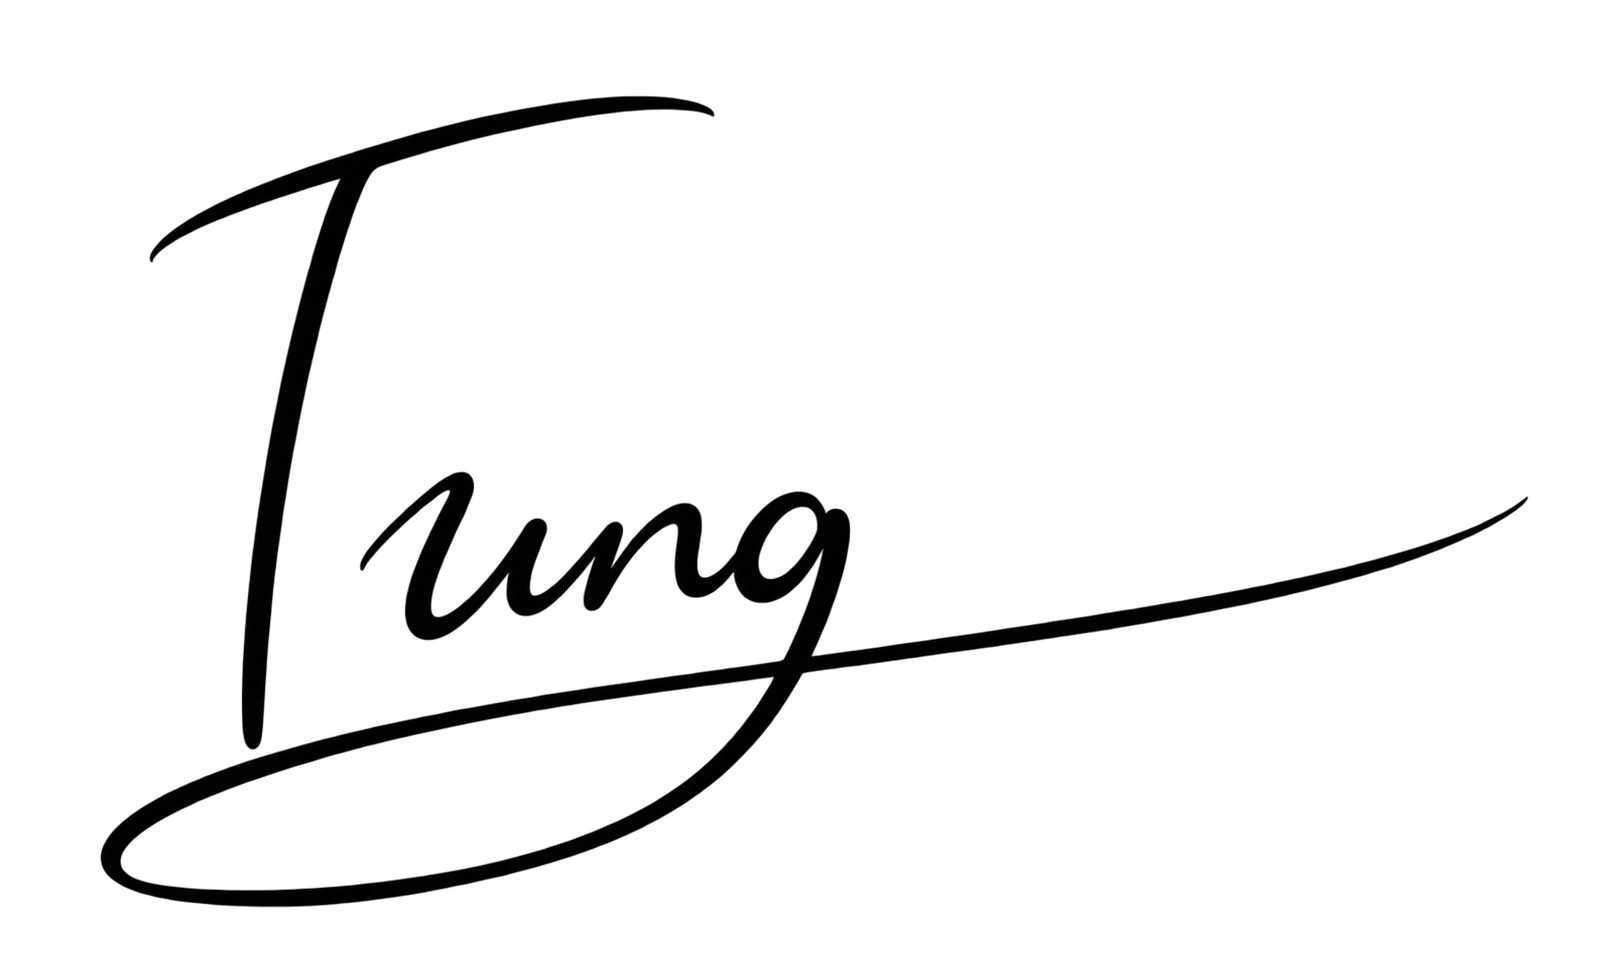
\includegraphics[width=4.2cm,height=2cm,keepaspectratio]{Hinhve/chu_ky_hoang_van_tung.png}
\end{minipage}\par
\end{minipage}\par

\clearpage
\chapter*{TÓM TẮT DỰ ÁN}
\addcontentsline{toc}{chapter}{TÓM TẮT DỰ ÁN}
RoomHub là ứng dụng hỗ trợ đặt và quản lý phòng học, phòng họp, nhằm tập trung việc đăng ký sử dụng, phê duyệt và bàn giao quyền tiếp cận phòng. Ứng dụng hướng đến giảng viên, cán bộ, người học và quản trị viên cơ sở vật chất, giúp người dùng theo dõi lịch phòng và giảm xung đột khi tổ chức hoạt động học tập, làm việc.

Người dùng có thể tra cứu phòng theo thời gian, tầng, sức chứa và thiết bị; đặt phòng một lần hoặc lặp theo tuần; theo dõi, chỉnh sửa và hủy yêu cầu. Quản trị viên quản lý tài khoản, phòng, quy định đặt phòng và bảo trì; xử lý yêu cầu bằng phê duyệt thủ công hoặc tự động. Quy trình tiếp cận phòng hỗ trợ hẹn nhận chìa, ủy quyền hoặc tạo mã PIN tạm thời; các chức năng điểm danh, ghi chú và thông báo giúp theo dõi quá trình sử dụng.

Giải pháp sử dụng React Native và TypeScript cho ứng dụng Android, Async Storage cho dữ liệu local và Spring Boot/H2 cho chế độ REST. Sản phẩm đã hoàn thiện các luồng nghiệp vụ chính, vận hành trên Android và kết nối SmartLock trong thử nghiệm thực tế. Hướng phát triển tiếp theo là mở rộng quy mô quản lý và trải nghiệm sử dụng.

\noindent\textbf{Từ khóa:} React Native; TypeScript; đặt phòng; quản lý phòng; SmartLock.

\phantomsection
\section*{THUẬT NGỮ VÀ TỪ VIẾT TẮT}
\addcontentsline{toc}{chapter}{THUẬT NGỮ VÀ TỪ VIẾT TẮT}
{\tabletext\setstretch{1.0}\renewcommand{\arraystretch}{1.04}
\begin{longtable}{>{\raggedright\arraybackslash}p{\dimexpr.17\textwidth-2\tabcolsep\relax}>{\raggedright\arraybackslash}p{\dimexpr.83\textwidth-2\tabcolsep\relax}}
\caption{Thuật ngữ sử dụng trong báo cáo}\\
\toprule\textbf{Thuật ngữ} & \textbf{Ý nghĩa trong ngữ cảnh dự án}\\\midrule
\endfirsthead
\toprule\textbf{Thuật ngữ} & \textbf{Ý nghĩa trong ngữ cảnh dự án}\\\midrule
\endhead
\bottomrule\endlastfoot
AES / CTR & Mã hóa payload PIN trong module MQTT native.\\\addlinespace[1.5pt]
API & Hợp đồng gọi dịch vụ; dự án dùng HTTP API của booking-server.\\\addlinespace[1.5pt]
APK & Gói cài Android; bản Release chứa JavaScript bundle.\\\addlinespace[1.5pt]
BR / FR / NFR & Quy tắc nghiệp vụ / yêu cầu chức năng / yêu cầu phi chức năng.\\\addlinespace[1.5pt]
CRUD & Tạo, đọc, sửa và xóa dữ liệu theo quyền.\\\addlinespace[1.5pt]
DI / IoC & Spring quản lý thành phần và truyền phụ thuộc cho filter/controller/service.\\\addlinespace[1.5pt]
DTO & Dữ liệu vào/ra dịch vụ; khác entity lưu trong H2.\\\addlinespace[1.5pt]
HTTP / REST & Giao tiếp API theo tài nguyên/phương thức, dùng JSON và Bearer token.\\\addlinespace[1.5pt]
IoT / oneM2M & Internet vạn vật / quy ước bản tin và chủ đề dùng với OneIoT.\\\addlinespace[1.5pt]
JPA / ORM & Ánh xạ entity Java tới dữ liệu quan hệ.\\\addlinespace[1.5pt]
JSON & Định dạng dữ liệu API, kho local và các trường lồng của booking.\\\addlinespace[1.5pt]
JVM & Máy ảo chạy backend Java 17.\\\addlinespace[1.5pt]
MQTT & Giao thức publish/subscribe qua broker; kết nối khóa từ native Android.\\\addlinespace[1.5pt]
PIN & Mã tạm bảy chữ số theo quyền phòng, booking và khoảng hiệu lực.\\\addlinespace[1.5pt]
PUBACK / QoS & Phản hồi broker khi nhận publish / mức chất lượng giao nhận MQTT.\\\addlinespace[1.5pt]
RN / TS & React Native / TypeScript; nền tảng giao diện và ngôn ngữ app.\\\addlinespace[1.5pt]
TLS & Bảo vệ kênh truyền; native hiện còn hạn chế xác minh chứng thư.\\\addlinespace[1.5pt]
UC / UML & Ca sử dụng / ký pháp mô hình hóa phân tích và thiết kế.\\\addlinespace[1.5pt]
UUID & Định danh duy nhất dạng chuỗi.\\\addlinespace[1.5pt]
Local / REST & Async Storage trên máy / API tới backend; hai kho không tự đồng bộ.\\\addlinespace[1.5pt]
\end{longtable}}

\clearpage
% Danh mục một cột, tách hình và bảng để dễ tra cứu.
\makeatletter
\chapter*{\contentsname}
{\small\setstretch{1.05}\@starttoc{toc}}
\clearpage
\chapter*{\listfigurename}
{\small\setstretch{1.0}\let\addvspace\@gobble\@starttoc{lof}}
\clearpage
\chapter*{\listtablename}
{\small\setstretch{1.0}\let\addvspace\@gobble\@starttoc{lot}}
\makeatother
\clearpage
\pagenumbering{arabic}
\chapter{GIỚI THIỆU DỰ ÁN}\label{chap:intro}
\section{Bối cảnh và bài toán thực tế}
RoomHub liên kết đặt phòng, phê duyệt và tiếp cận phòng theo vai trò user/admin, thay cho đối chiếu lịch và bàn giao khóa rời rạc qua bảng tính hoặc trao đổi trực tiếp \cite{quytrinh2026}. Khóa cơ/thẻ có hẹn nhận, ủy quyền và điểm danh; khóa số có quyền PIN theo thời hạn; người đang dùng phòng được báo tình trạng/bảo trì.

C7, Đại học Bách khoa Hà Nội là ví dụ tham chiếu của đề xuất. Dữ liệu minh họa do nhóm xây dựng gồm tám tầng, bảy phòng mỗi tầng, cùng thông tin sức chứa và thiết bị.

\section{Mục tiêu và tiêu chí nghiệm thu}
{\tabletext\renewcommand{\arraystretch}{1.04}\begin{longtable}{>{\raggedright\arraybackslash}p{\dimexpr0.27\textwidth-2\tabcolsep\relax}>{\raggedright\arraybackslash}p{\dimexpr0.34\textwidth-2\tabcolsep\relax}>{\raggedright\arraybackslash}p{\dimexpr0.39\textwidth-2\tabcolsep\relax}}
\caption{Mục tiêu, cách xác minh và mức kết quả}\label{tab:goals}\\
\toprule \textbf{Mã / mục tiêu} & \textbf{Cách kiểm chứng} & \textbf{Kết quả có căn cứ}\\\midrule
\endfirsthead
\multicolumn{3}{l}{\small Mục tiêu, cách xác minh và mức kết quả (tiếp)}\\
\toprule \textbf{Mã / mục tiêu} & \textbf{Cách kiểm chứng} & \textbf{Kết quả có căn cứ}\\\midrule
\endhead
\bottomrule\endlastfoot
G01 -- Đặt phòng hợp lệ & Đăng nhập, lọc phòng, gửi yêu cầu; test trùng lịch, bảo trì và hạn mức. & Luồng tìm, đặt phòng và các quy tắc xung đột, bảo trì, hạn mức hoạt động đúng trong ứng dụng.\\\addlinespace[1.5pt]
G02 -- Duyệt và tiếp cận & Duyệt tay/tự động, quyền PIN theo phòng, nhận chìa, no-show. & Hoàn thành luồng duyệt, cấp quyền và sử dụng PIN với SmartLock trong chạy thử thực tế.\\\addlinespace[1.5pt]
G03 -- Trải nghiệm Android & Bản Release chạy không cần Metro; màn hình theo vai trò và thông báo đúng người nhận. & Ứng dụng Android chạy độc lập Metro, hiển thị chức năng đúng vai trò và xử lý thông báo.\\\addlinespace[1.5pt]
G04 -- Tái lập và phối hợp & README, lockfile, test, lịch sử Git và minh chứng từng thành viên. & README mô tả cài đặt và cấu hình; lockfile cố định phụ thuộc; bộ kiểm thử và hồ sơ bàn giao hỗ trợ tái lập bản chạy Android.\\\addlinespace[1.5pt]
\end{longtable}}

\section{Đối tượng, phạm vi và giả định}
Người dùng mục tiêu là giảng viên, cán bộ hoặc người học; vai trò user đại diện cho nhóm đặt và sử dụng phòng, còn admin quản lý tài nguyên. Giao diện dùng nhãn GIẢNG VIÊN cho vai trò user theo bối cảnh phòng học của dữ liệu thử. Phạm vi gồm tài khoản/hồ sơ, phòng, booking một lần/lặp tuần, duyệt, PIN/hẹn chìa, điểm danh, bảo trì, ghi chú, thông báo và cấu hình.

Giả định đồng hồ đúng, phòng đã khai báo và có một loại khóa. Mặc định đặt trước 1--3 ngày, tối đa 2 lượt hoạt động; admin đổi được. REST cần server/URL khả dụng; local không hòa giải dữ liệu với server. Mở rộng nhiều tòa nhà/khóa, server push và tự động hóa quản lý PIN là các hướng phát triển tiếp theo.

\section{Sản phẩm bàn giao}
Sản phẩm bàn giao gồm ứng dụng Android để đặt và quản lý phòng; mã nguồn ứng dụng và backend Java để cài đặt, vận hành và phát triển tiếp; README hướng dẫn cấu hình, build và chạy thử; dữ liệu mẫu, bộ kiểm thử, ảnh giao diện, sơ đồ và báo cáo. Mã nguồn được lưu tại nhánh main của repository nhóm \cite{roomhubrepo}. Danh mục minh chứng và kịch bản demo nằm ở Phụ lục~\ref{app:evidence}; phần việc thành viên ở Phụ lục~\ref{app:contributions}.

\FloatBarrier
\chapter{KHẢO SÁT VÀ ĐẶC TẢ YÊU CẦU}\label{chap:requirements}
\section{Bối cảnh khảo sát và mô hình nghiệp vụ}
\subsection{Quy trình tham chiếu và phạm vi dữ liệu}
Phương pháp khảo sát là phân tích quy trình nghiệp vụ tham chiếu của nhóm \cite{quytrinh2026}, từ đó xác định tác nhân, trường hợp sử dụng, trạng thái và quyền thao tác. Dữ liệu phòng do nhóm xây dựng để mô hình hóa tình huống; đây là khảo sát quy trình và phân tích yêu cầu, không phải nghiên cứu thống kê người dùng.

Hai vai trò tài khoản là \code{user} và \code{admin}; OneIoT là hệ thống khóa bên ngoài. Dữ liệu tám tầng/bảy phòng mỗi tầng phục vụ kiểm tra giao diện và lọc phòng.

\subsection{Phương thức tiếp cận phòng trong bản triển khai}
Mỗi phòng có một loại khóa \code{PHYSICAL_KEY} hoặc \code{PIN_CODE} (Bảng~\ref{tab:access-modes}); người đặt không tự đổi phương thức khóa cho một lượt.
{\tabletext\renewcommand{\arraystretch}{1.04}\begin{longtable}{>{\raggedright\arraybackslash}p{\dimexpr0.24\textwidth-2\tabcolsep\relax}>{\raggedright\arraybackslash}p{\dimexpr0.43\textwidth-2\tabcolsep\relax}>{\raggedright\arraybackslash}p{\dimexpr0.33\textwidth-2\tabcolsep\relax}}
\caption{Hai phương thức tiếp cận được model hỗ trợ}\label{tab:access-modes}\\
\toprule \textbf{Loại khóa} & \textbf{Luồng sau khi duyệt} & \textbf{Đặc điểm vận hành}\\\midrule
\endfirsthead
\multicolumn{3}{l}{Hai phương thức tiếp cận (tiếp)}\\
\toprule \textbf{Loại khóa} & \textbf{Luồng sau khi duyệt} & \textbf{Đặc điểm vận hành}\\\midrule
\endhead
\bottomrule\endlastfoot
Khóa cơ/thẻ & User đề xuất giờ nhận; admin chấp nhận hoặc đề xuất lại; có thể khai báo người nhận hộ. Admin xác nhận có mặt trong giờ sử dụng. & Lịch hẹn và ủy quyền hỗ trợ bàn giao chìa; việc trả chìa được thực hiện theo quy trình quản lý phòng.\\\addlinespace[1.5pt]
Khóa số & Phòng được gắn SmartLock; người có quyền tạo PIN theo booking và thời hạn; mã chờ hoặc được gửi qua OneIoT. & Ứng dụng lưu PIN, gửi lệnh qua OneIoT và tiếp nhận sự kiện sử dụng khóa theo phiên kết nối.\\\addlinespace[1.5pt]
\end{longtable}}

\section{Tác nhân, kịch bản sử dụng và luồng nghiệp vụ}
\subsection{Phạm vi của từng tác nhân}
Hình~\ref{fig:uc-overview} mô tả chức năng chung: user quản lý lượt của mình, admin xử lý yêu cầu/tài nguyên. Repository local hoặc filter/service server tiếp tục kiểm quyền sau UI.
\begin{figure}[!htbp]\centering
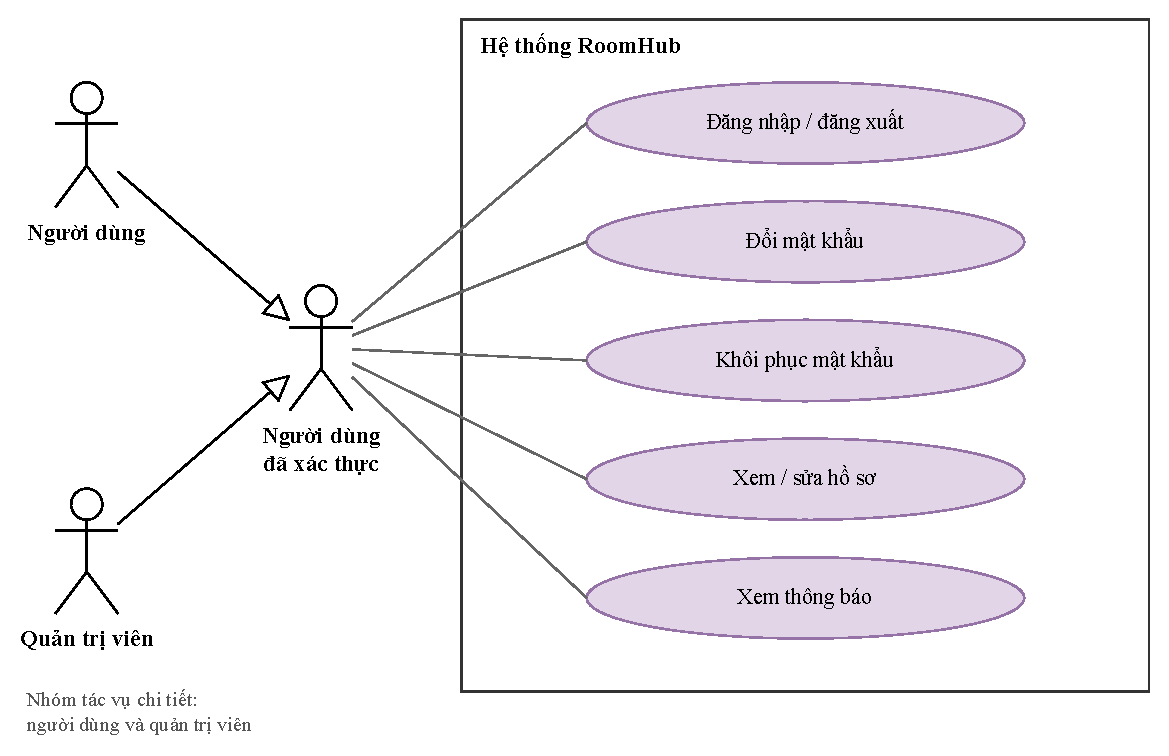
\includegraphics[width=\textwidth,height=.40\textheight,keepaspectratio]{Hinhve/design/02a_use_case_tong_quat.pdf}
\caption{Các use case chung và hai vai trò của RoomHub}\label{fig:uc-overview}
\end{figure}

Hình~\ref{fig:uc-user} tách tác vụ user. Mọi yêu cầu đặt đều được kiểm quy tắc trước nhánh tự duyệt, không do user tự cấp quyền.
\begin{figure}[!htbp]\centering
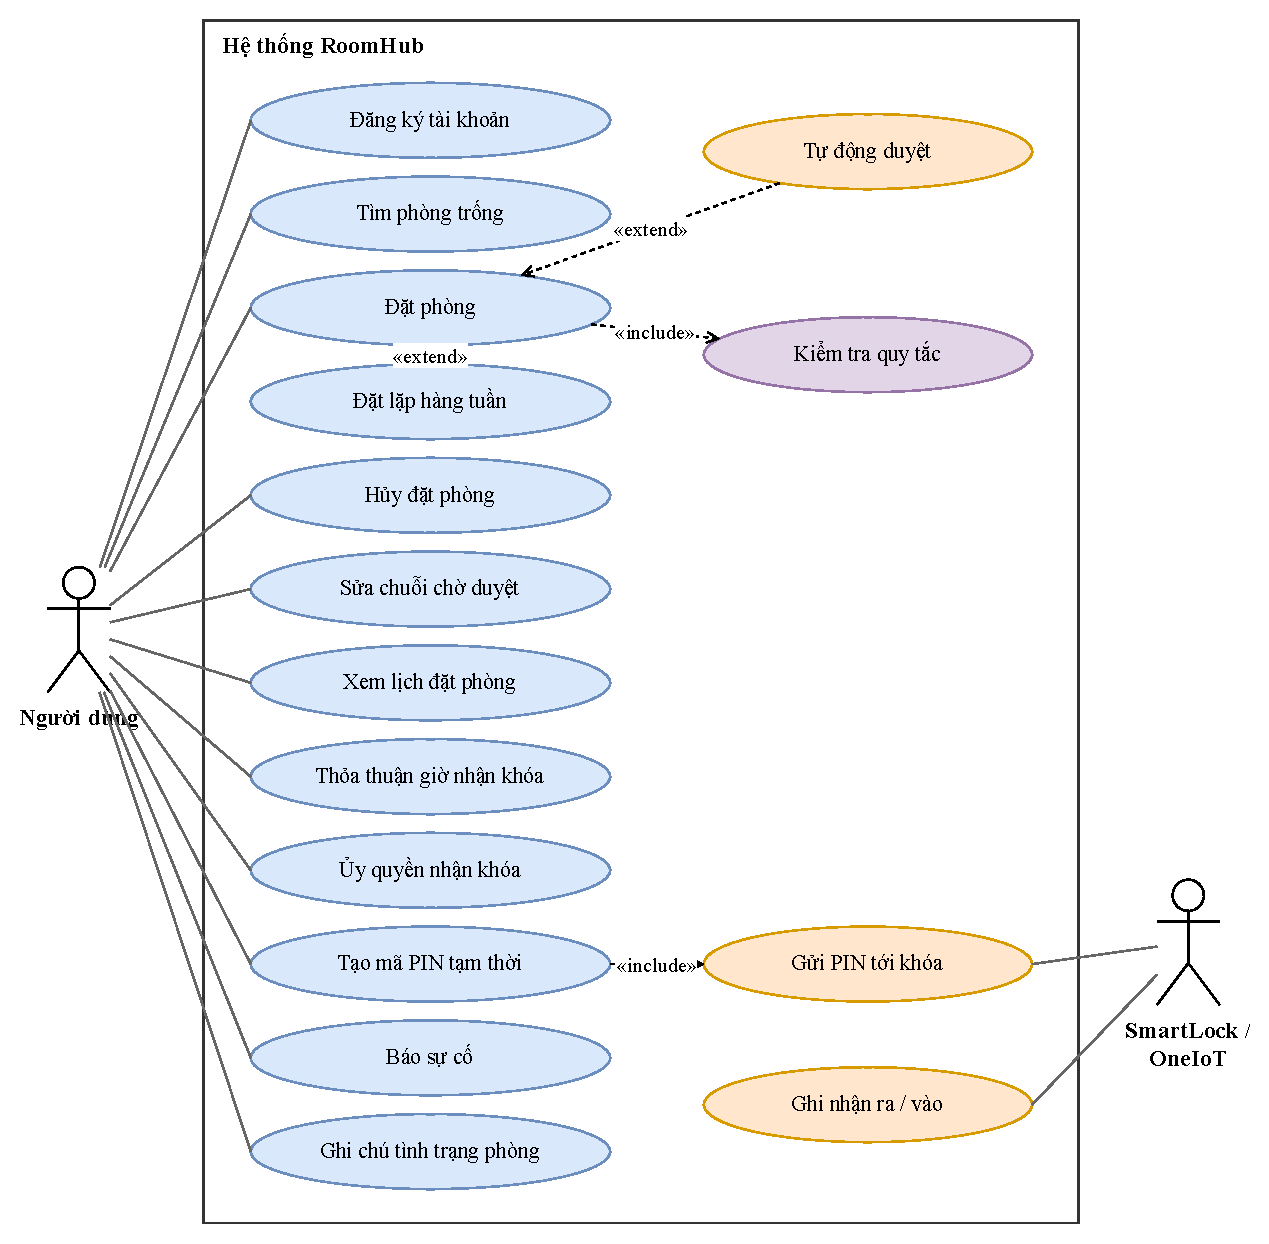
\includegraphics[width=\textwidth,height=.50\textheight,keepaspectratio]{Hinhve/design/02b_use_case_nguoi_dung.pdf}
\caption{Use case của người dùng và tương tác với hệ thống khóa}\label{fig:uc-user}
\end{figure}

Hình~\ref{fig:uc-admin} mô tả tác vụ admin; cấp/thu hồi quyền PIN theo cặp user--phòng không đổi vai trò tài khoản.
\begin{figure}[!htbp]\centering
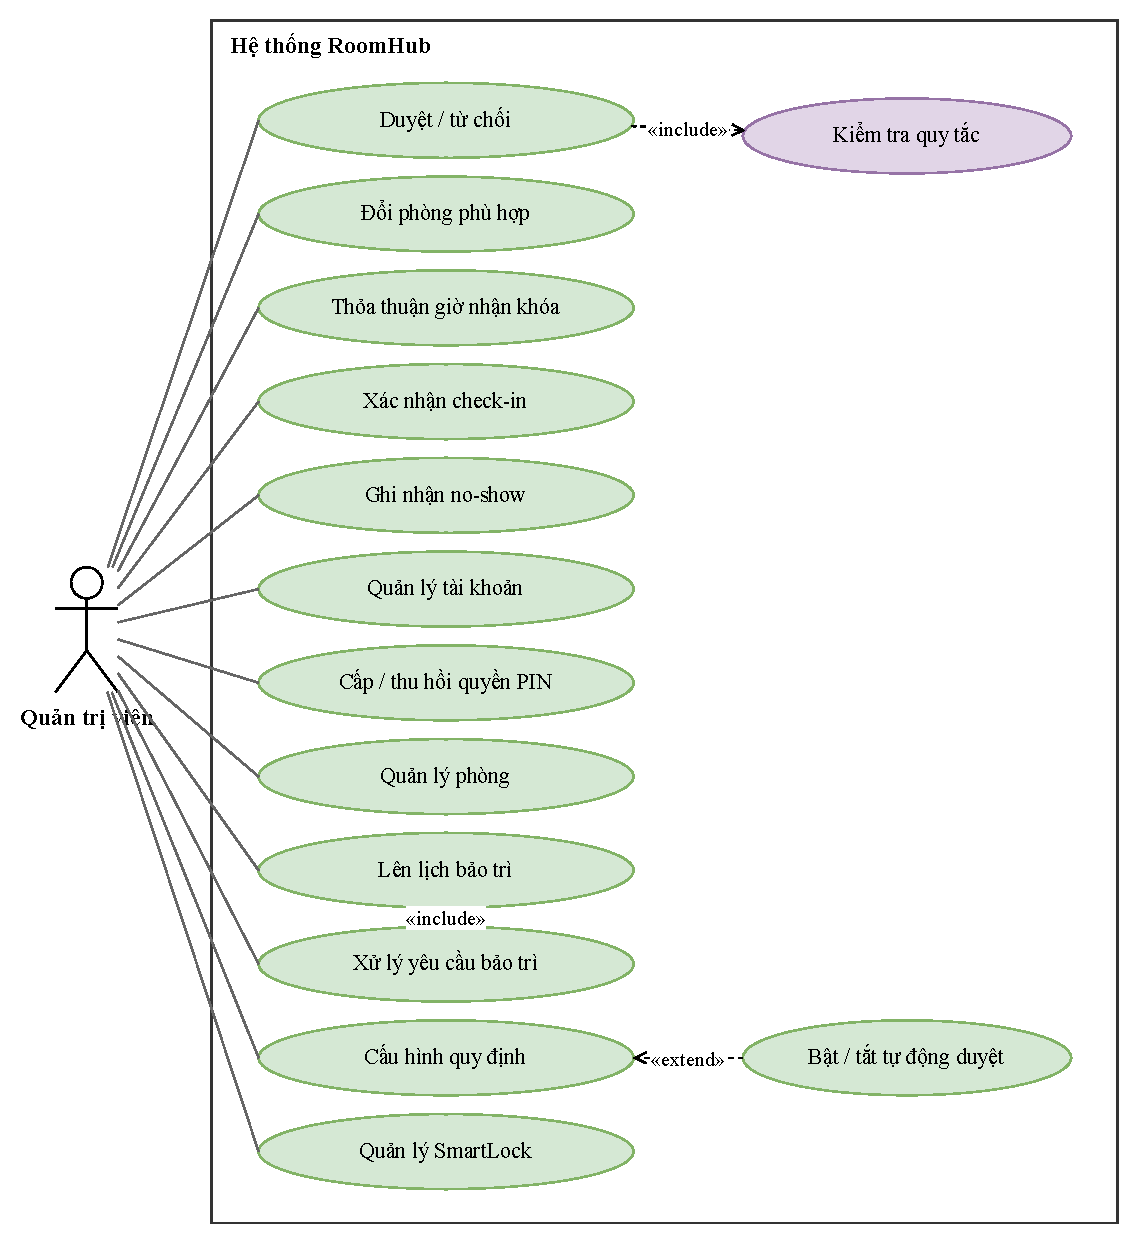
\includegraphics[width=\textwidth,height=.49\textheight,keepaspectratio]{Hinhve/design/02c_use_case_quan_tri_vien.pdf}
\caption{Use case quản trị tài nguyên và xử lý yêu cầu}\label{fig:uc-admin}
\end{figure}
\FloatBarrier

\subsection{Ba kịch bản nghiệp vụ tiêu biểu}
Ba tuyến nghiệp vụ là: đặt/duyệt phòng PIN (UC02, UC03, UC05); nhận chìa, ủy quyền và điểm danh/no-show (UC07, UC12); ghi chú và xử lý bảo trì trong giờ dùng (UC08, UC13). Điều kiện và ngoại lệ được đặc tả tại mục~\ref{sec:use-case-spec}.

\subsection{Đặt phòng, tự duyệt và cấp quyền tiếp cận}
Hình~\ref{fig:activity} thể hiện nhánh REST: UI gửi API, server kiểm điều kiện trước khi quyết định tự duyệt hoặc chuyển admin. Nhánh local thực hiện cùng nhóm quy tắc qua repository thay cho HTTP. Với chuỗi tuần, mọi buổi đều được kiểm xung đột trước khi chốt lưu.
\begin{figure}[H]\centering
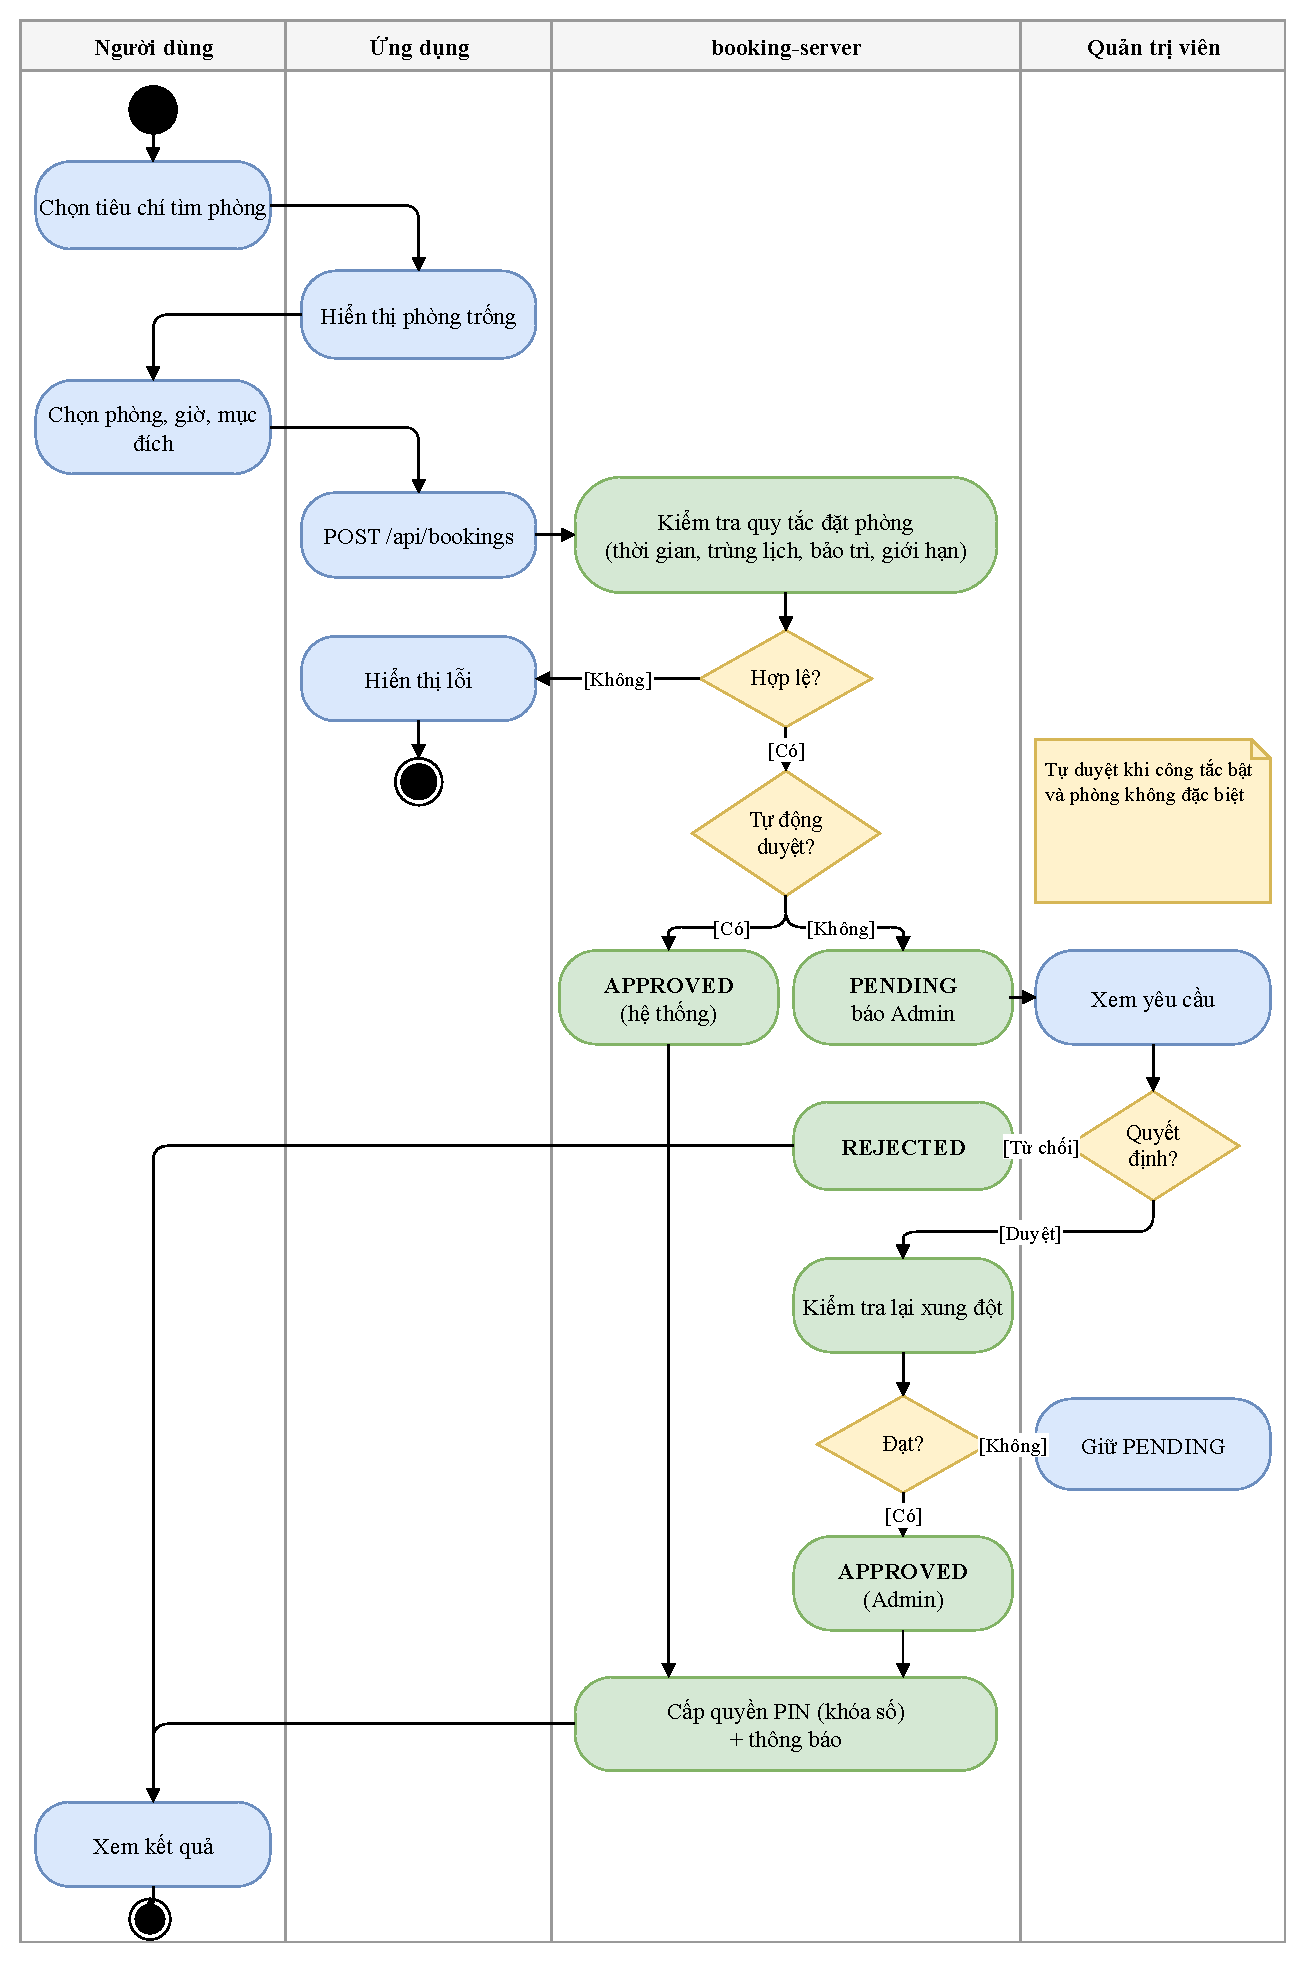
\includegraphics[width=\textwidth,height=.68\textheight,keepaspectratio]{Hinhve/design/03_activity_dat_phong_duyet.pdf}
\caption{Luồng tạo yêu cầu và quyết định duyệt trong nhánh REST}\label{fig:activity}
\end{figure}

Hình~\ref{fig:activity-pin} tách sinh/lưu PIN và gửi lệnh tới khóa. PIN có bảy chữ số; thời hạn lấy từ booking và khoảng đệm cấu hình. Thuộc tính \code{lockDeliveredAt} lưu thời điểm broker nhận lệnh gửi mã. Luồng app--OneIoT--SmartLock đã được nhóm chạy thực tế để sử dụng mã và thao tác khóa.


\begin{figure}[H]\centering
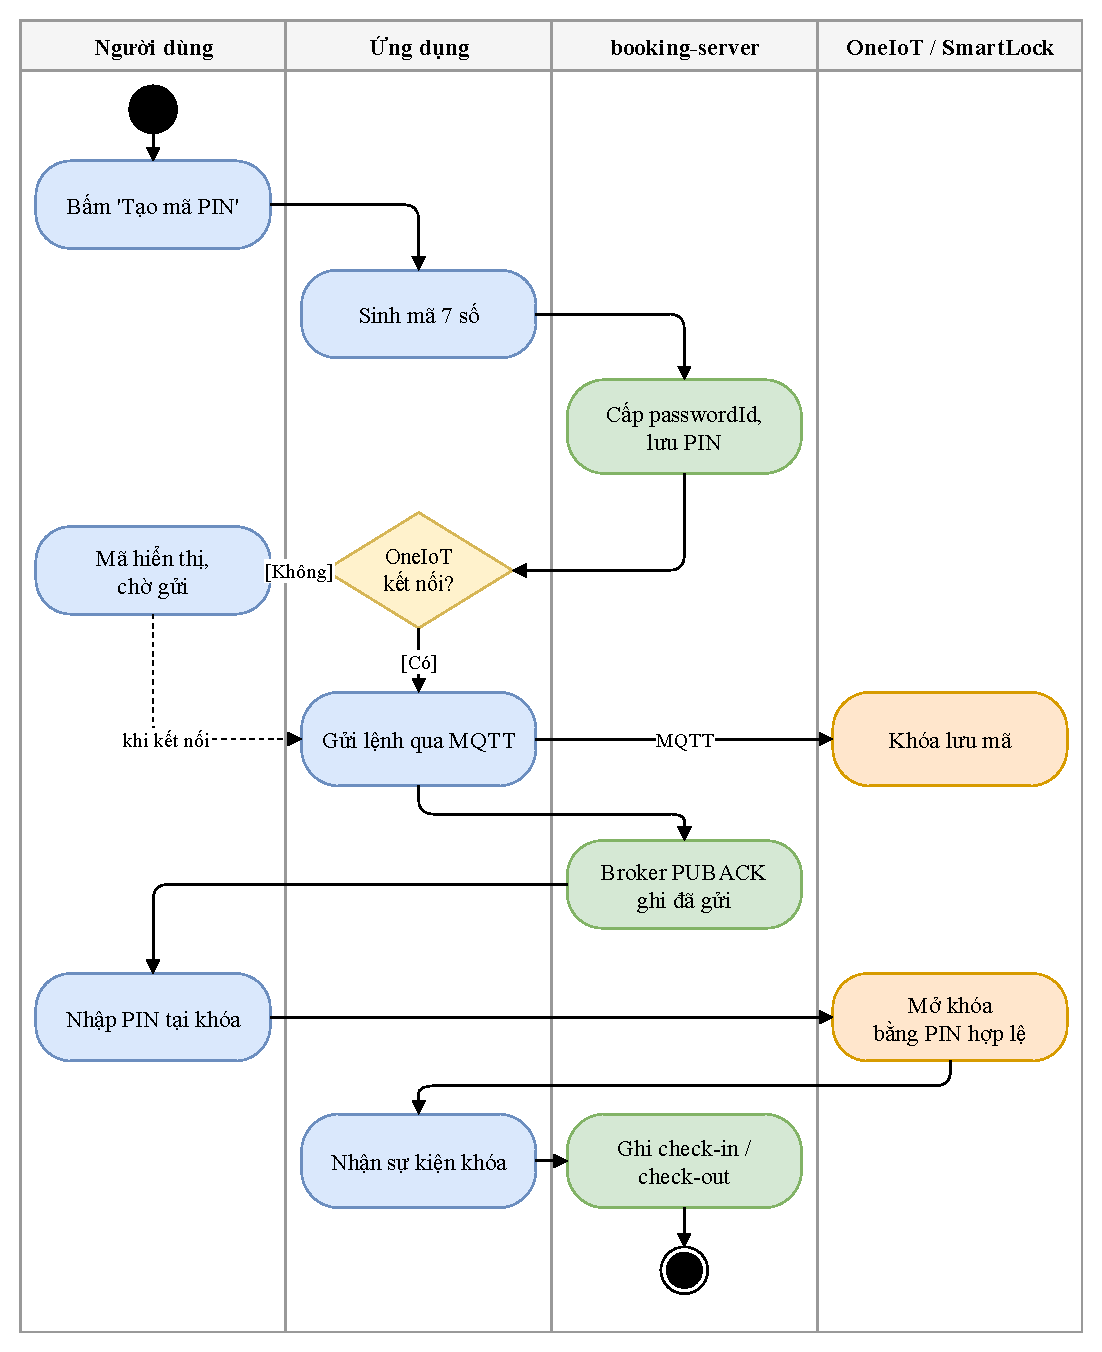
\includegraphics[width=\textwidth,height=.56\textheight,keepaspectratio]{Hinhve/design/04a_activity_khoa_so_pin.pdf}
\caption{Luồng tạo PIN, chờ gửi và giao tiếp OneIoT}\label{fig:activity-pin}
\end{figure}

Hình~\ref{fig:activity-key} giữ riêng lịch nhận khóa, có mặt/vắng mặt và xử lý bảo trì. Lịch hẹn phải ở tương lai và trước giờ sử dụng; check-in thủ công chỉ được ghi trong giờ dùng. Có mặt muộn vẫn có thể được xác nhận nếu booking đang hợp lệ và chưa bị admin đóng bằng no-show.

\begin{figure}[H]\centering
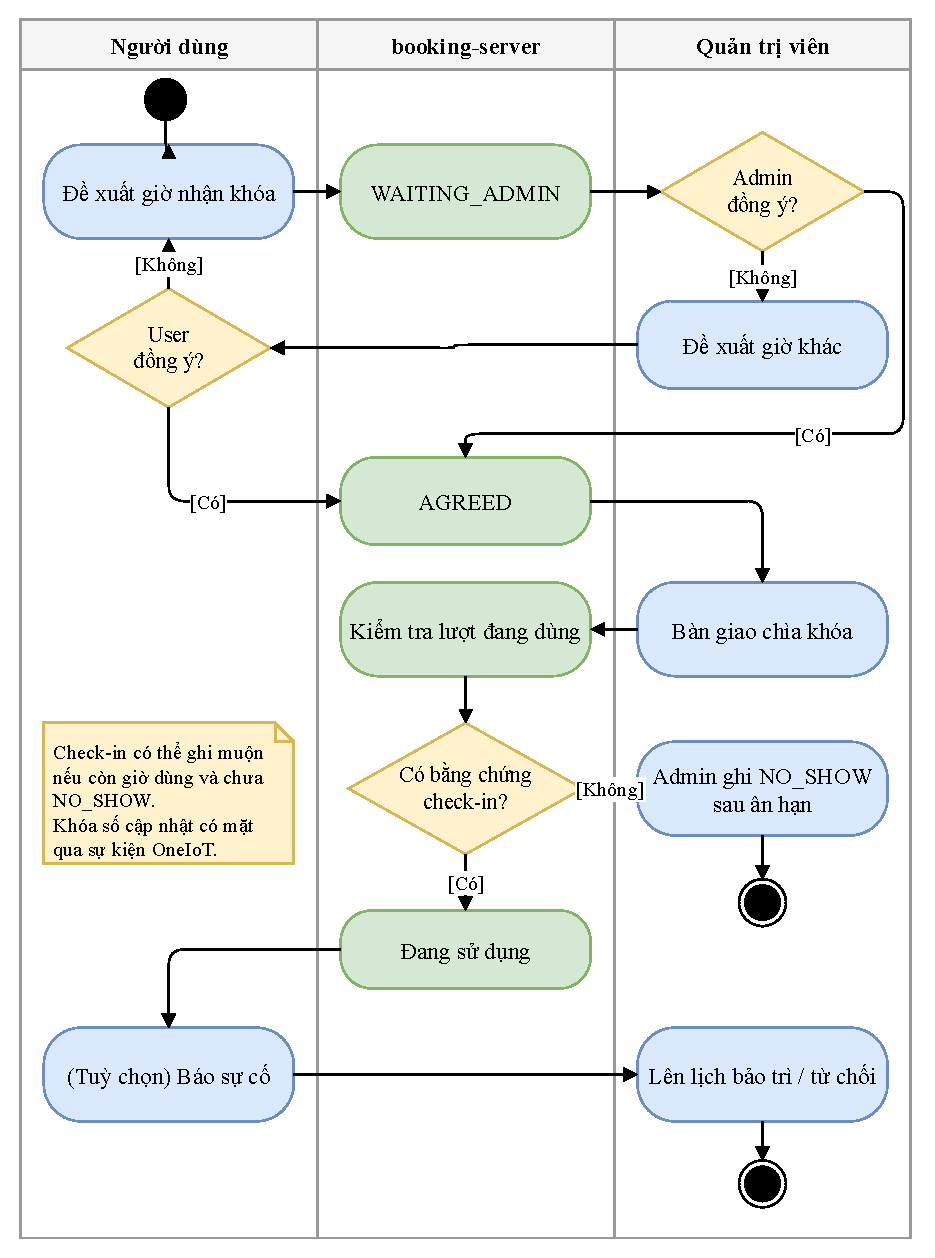
\includegraphics[width=\textwidth,height=.56\textheight,keepaspectratio]{Hinhve/design/04b_activity_khoa_co_vang_mat_bao_tri.pdf}
\caption{Thỏa thuận nhận khóa, xác nhận có mặt và xử lý bảo trì}\label{fig:activity-key}
\end{figure}

\subsection{Vòng đời trạng thái đặt phòng}
Trạng thái lưu là \code{PENDING}, \code{APPROVED}, \code{REJECTED}, \code{CANCELLED} và \code{NO_SHOW}. Tự duyệt cho phép tạo thẳng \code{APPROVED}. Check-in/check-out là các trường/sự kiện bên trong một lượt đã duyệt; đổi phòng không tự đổi trạng thái. Khi hết giờ, UI phân nhóm lượt đã dùng theo thời gian, không ghi thêm trạng thái \code{COMPLETED} vào model. Hình~\ref{fig:booking-state} thể hiện các trạng thái lưu và sự kiện sử dụng của lượt đặt.
\begin{figure}[H]\centering
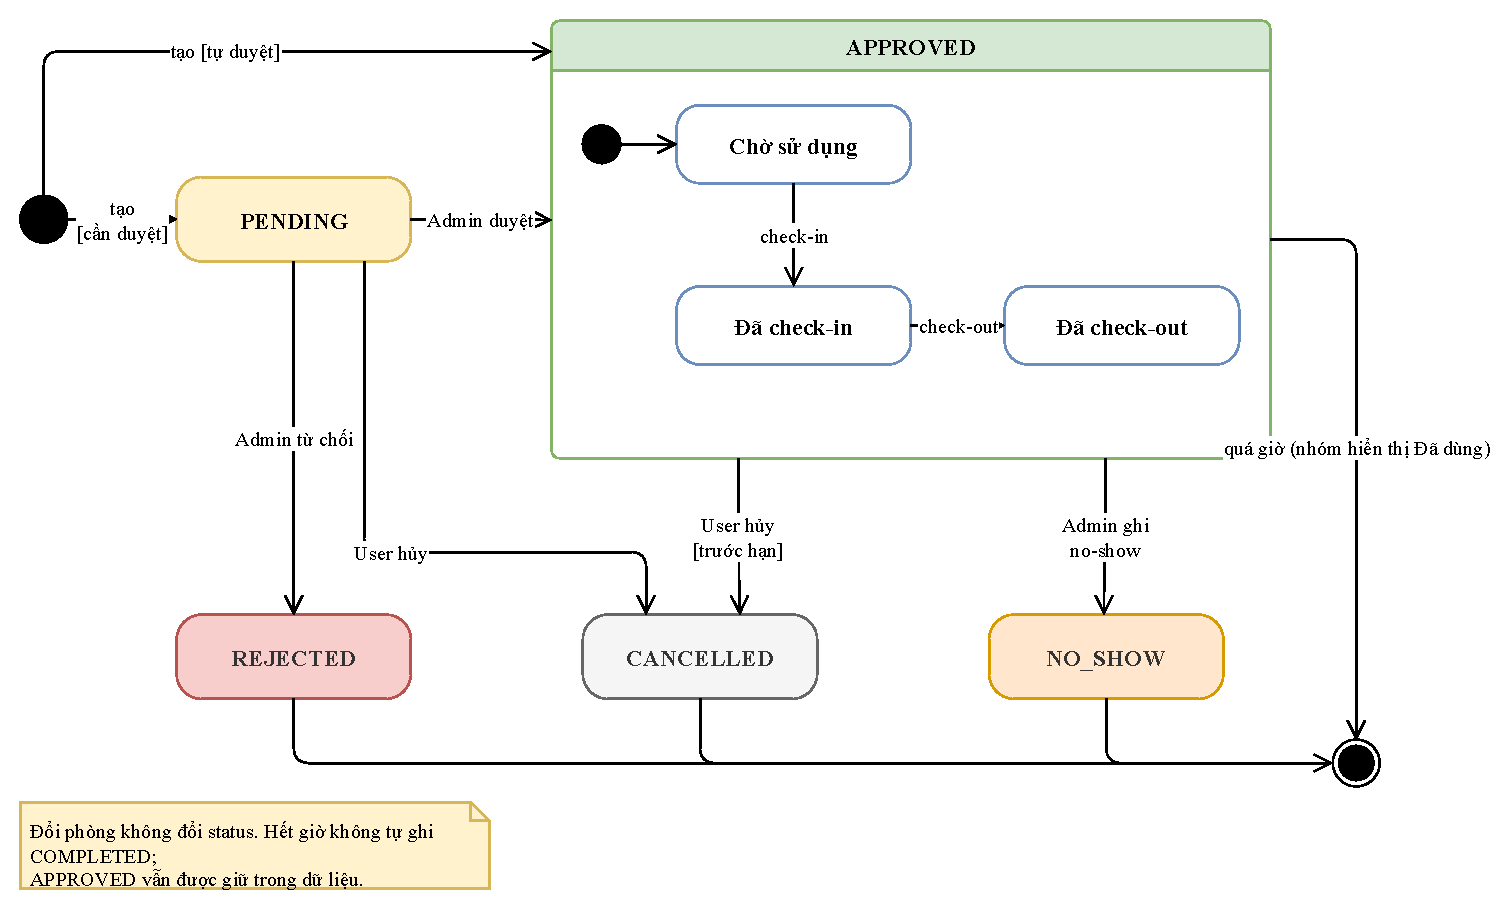
\includegraphics[width=\textwidth,height=.40\textheight,keepaspectratio]{Hinhve/design/18a_state_booking.pdf}
\caption{Vòng đời booking và các mốc sử dụng liên quan}\label{fig:booking-state}
\end{figure}
\FloatBarrier

\section{Yêu cầu chức năng}
{\tabletext\renewcommand{\arraystretch}{1.04}\begin{longtable}{>{\raggedright\arraybackslash}p{\dimexpr0.14\textwidth-2\tabcolsep\relax}>{\raggedright\arraybackslash}p{\dimexpr0.47\textwidth-2\tabcolsep\relax}>{\raggedright\arraybackslash}p{\dimexpr0.39\textwidth-2\tabcolsep\relax}}
\caption{Yêu cầu chức năng và minh chứng kiểm thử}\label{tab:fr}\\
\toprule \textbf{ID / ưu tiên} & \textbf{Yêu cầu và luồng chính} & \textbf{Minh chứng hiện có}\\\midrule
\endfirsthead
\multicolumn{3}{l}{\small Yêu cầu chức năng và minh chứng kiểm thử (tiếp)}\\
\toprule \textbf{ID / ưu tiên} & \textbf{Yêu cầu và luồng chính} & \textbf{Minh chứng hiện có}\\\midrule
\endhead
\bottomrule\endlastfoot
FR01 / Cao & Đăng ký, đăng nhập, đổi/khôi phục mật khẩu; đọc role từ tài khoản. & Ảnh Hình~\ref{fig:ui-roles}; TC01, TC17 và D01--D03.\\\addlinespace[1.5pt]
FR02 / Cao & Tìm phòng theo tầng, giờ, sức chứa, thiết bị, loại khóa; trạng thái theo lịch. & Ảnh Hình~\ref{fig:ui-booking}; TC02, TC12.\\\addlinespace[1.5pt]
FR03 / Cao & Tạo booking một lần/lặp; chặn trùng lịch và bảo trì; hủy/sửa chuỗi theo điều kiện. & TC02, TC11--TC12, TC21; kiểm thử quy tắc và vòng đời đặt phòng.\\\addlinespace[1.5pt]
FR04 / Cao & Admin duyệt/từ chối/đổi phòng; tự duyệt phòng thường khi bật công tắc. & TC07, TC20, TC24; kiểm thử tự duyệt, duyệt tay và đổi phòng.\\\addlinespace[1.5pt]
FR05 / Cao & Quyền PIN theo user--phòng, PIN 7 số và thời hạn; hẹn nhận chìa/ủy quyền. & TC03, TC10, TC13--TC15, TC19; thử nghiệm app--SmartLock.\\\addlinespace[1.5pt]
FR06 / Trung bình & Ghi nhận sự kiện khóa, check-in thủ công khóa cơ và no-show có điều kiện. & TC10, TC22; kiểm thử sự kiện, check-in và ngưỡng no-show.\\\addlinespace[1.5pt]
FR07 / Cao & Tách ghi chú với yêu cầu bảo trì; admin xử lý lịch/yêu cầu. & Ảnh Hình~\ref{fig:ui-room-maintenance}; TC02, TC23.\\\addlinespace[1.5pt]
FR08 / Cao & Admin quản lý tài khoản/phòng/cấu hình; user sửa hồ sơ và xem thông báo. & Ảnh Hình~\ref{fig:ui-roles}; TC06, TC08--TC09, TC16, TC18.\\\addlinespace[1.5pt]
\end{longtable}}

\section{Quy tắc nghiệp vụ và các trường hợp biên}
Bảng~\ref{tab:br} trình bày các mã BR để đặc tả và kiểm thử tham chiếu cùng một quy tắc. Giá trị trong bảng là mặc định của model cấu hình, không phải hằng số cố định cho mọi lần sử dụng.
{\tabletext\renewcommand{\arraystretch}{1.04}\begin{longtable}{>{\raggedright\arraybackslash}p{\dimexpr0.12\textwidth-2\tabcolsep\relax}>{\raggedright\arraybackslash}p{\dimexpr0.66\textwidth-2\tabcolsep\relax}>{\raggedright\arraybackslash}p{\dimexpr0.22\textwidth-2\tabcolsep\relax}}
\caption{Quy tắc nghiệp vụ đối chiếu với mã nguồn}\label{tab:br}\\
\toprule \textbf{Mã} & \textbf{Điều kiện xử lý} & \textbf{Giá trị / phạm vi}\\\midrule
\endfirsthead
\multicolumn{3}{l}{Quy tắc nghiệp vụ (tiếp)}\\
\toprule \textbf{Mã} & \textbf{Điều kiện xử lý} & \textbf{Giá trị / phạm vi}\\\midrule
\endhead
\bottomrule\endlastfoot
BR-01 & Phòng phải tồn tại và có trạng thái cho phép đặt; phương thức tiếp cận lấy từ loại khóa của phòng. & \code{AVAILABLE}.\\\addlinespace[1.5pt]
BR-02 & Ngày/giờ hợp lệ, bắt đầu trước kết thúc; giao nhau dùng khoảng nửa mở nên hai lượt liền kề không xung đột. & Cùng ngày, start trước end.\\\addlinespace[1.5pt]
BR-03 & Cửa sổ đặt trước áp dụng cho lượt đầu; khoảng dùng chưa kết thúc. Min bằng 0 cho phép cùng ngày đã bắt đầu nhưng còn thời gian. & Mặc định 1--3 ngày.\\\addlinespace[1.5pt]
BR-04 & Không chồng lịch bảo trì chưa hủy của đúng phòng. & Áp dụng từng buổi.\\\addlinespace[1.5pt]
BR-05 & Không trùng lượt còn hoạt động của cùng phòng hoặc cùng user; các trạng thái giữ chỗ là PENDING/APPROVED. & Kiểm theo khoảng giờ.\\\addlinespace[1.5pt]
BR-06 & Mục đích không trống; hạn mức kiểm ở lượt đầu khi tạo chuỗi, không cộng lại điều kiện hạn mức cho từng tuần tiếp theo. & Mặc định 2 lượt; chuỗi UI 1--8 tuần.\\\addlinespace[1.5pt]
BR-07 & Duyệt tay chỉ cho lượt PENDING chưa hết giờ; kiểm lại bảo trì và lịch đã duyệt. Tự duyệt chỉ sau validation, công tắc bật và phòng không đặc biệt. & Công tắc mặc định tắt.\\\addlinespace[1.5pt]
BR-08 & Chỉ chủ lượt hủy PENDING/APPROVED trước khi bắt đầu; lượt đã duyệt còn phải thỏa hạn hủy. & Mặc định 30 phút.\\\addlinespace[1.5pt]
BR-09 & Admin đổi lượt APPROVED trước hạn; phòng khác khả dụng, cùng loại khóa, đủ sức chứa/thiết bị, không xung đột/bảo trì; có lý do. & Mặc định 30 phút.\\\addlinespace[1.5pt]
BR-10 & PIN chỉ cho lượt đã duyệt ở phòng khóa số đang gắn SmartLock, chưa kết thúc và chưa có PIN chưa thu hồi. & 7 số; đệm mặc định 10 phút.\\\addlinespace[1.5pt]
BR-11 & User tạo PIN phải là chủ lượt và có quyền active đúng phòng; admin có thể cấp/thu hồi quyền cặp user--phòng. & Không đổi vai trò tài khoản.\\\addlinespace[1.5pt]
BR-12 & Thỏa thuận/ủy quyền nhận khóa chỉ cho lượt đã duyệt dùng khóa cơ/thẻ; lịch nhận ở tương lai và trước giờ dùng. & Admin xác nhận địa điểm.\\\addlinespace[1.5pt]
BR-13 & Check-in thủ công cho khóa cơ/thẻ trong giờ dùng; no-show chỉ khi đã qua ân hạn và chưa có bằng chứng check-in. & Ân hạn mặc định 15 phút.\\\addlinespace[1.5pt]
BR-14 & Ghi chú hoặc yêu cầu bảo trì do chủ lượt APPROVED gửi trong giờ sử dụng; chỉ yêu cầu bảo trì có vòng đời xử lý riêng. & Ghi chú tối đa 500 ký tự.\\\addlinespace[1.5pt]
\end{longtable}}

Một số khác biệt giữa hai chế độ dữ liệu và phạm vi xử lý gồm:
\begin{itemize}
\item Đặt lặp là dãy cách nhau bảy ngày. UI giới hạn 1--8 tuần; khi bị gọi trực tiếp, service local chặn giá trị nhỏ hơn 1 nhưng kẹp giá trị trên 8 về 8, còn backend từ chối ngoài 1--8.
\item Hủy, đổi phòng hoặc no-show cập nhật \code{revokedAt} để dừng sử dụng PIN của lượt đặt trong ứng dụng. Quyền room--user được quản lý riêng với PIN của từng booking.
\item Local thực hiện read--validate--write trên Async Storage; REST kiểm quyền theo phiên và dùng transaction/khóa ở backend. Hai nhánh không có cơ chế đồng bộ hay hòa giải dữ liệu tự động.
\end{itemize}

\section{Đặc tả các use case}\label{sec:use-case-spec}
Các mục~\ref{tab:uc01}--\ref{tab:uc11} đặc tả các tác vụ tài khoản, đặt phòng, tiếp cận phòng và quản trị. Mục~\ref{tab:uc12}--\ref{tab:uc13} mô tả điểm danh/no-show và ghi chú phòng. Mã FR liên kết với Bảng~\ref{tab:fr}, mã BR liên kết với Bảng~\ref{tab:br}. Vị trí triển khai và kỹ thuật xử lý được tổng hợp tại Chương~\ref{chap:implementation}.
\Needspace{16\baselineskip}
\subsection{UC01 -- Đăng nhập và các nhánh tài khoản}\label{tab:uc01}
{\small\renewcommand{\arraystretch}{1.06}
\setlength{\tabcolsep}{6pt}\setlength{\extrarowheight}{2pt}
\arrayrulecolor{black!35}
\renewcommand{\theHtable}{uc.\arabic{subsection}}\addtocounter{table}{-1}
\begin{longtable}{|>{\bfseries\raggedright\arraybackslash}p{3cm}|>{\raggedright\arraybackslash}p{\dimexpr\textwidth-3cm-4\tabcolsep-3\arrayrulewidth\relax}|}
\hline
\textbf{Trường} & \textbf{Nội dung đặc tả}\\\hline
\endfirsthead
\multicolumn{2}{r}{\small\itshape UC01 (tiếp)}\\
\hline
\textbf{Trường} & \textbf{Nội dung đặc tả}\\\hline
\endhead
\endlastfoot
Yêu cầu / quy tắc & FR01\\*\hline
Tác nhân & Người dùng và quản trị viên.\\*\hline
Tiền điều kiện & Tài khoản đăng nhập đã tồn tại và đang hoạt động; nhánh đăng ký tạo tài khoản user mới.\\*\hline
Luồng chính & 1. Nhập tên đăng nhập và mật khẩu; hệ thống kiểm các ô bắt buộc và thực hiện xác thực.\par
2. Chuẩn hóa username, kiểm mật khẩu và active. Local đọc kho tài khoản; REST gọi API và nhận token/username/role.\par
3. Lưu phiên trong bộ nhớ ứng dụng và mở dashboard tương ứng vai trò; những request cần xác thực mang token của phiên.\par
4. Khi đăng xuất, xóa phiên/token và ngắt kết nối OneIoT theo vòng đời app.\\\hline
Ngoại lệ / nhánh khác & Sai thông tin/tài khoản khóa: không tạo phiên. REST lỗi mạng/timeout: giữ form và báo lỗi, không tự chuyển local. Đăng ký kiểm username 3--30 ký tự theo tập cho phép, mật khẩu ít nhất 4 ký tự, hai mật khẩu khớp; họ tên và email là thông tin tùy chọn. Mã khôi phục là mã tĩnh của tài khoản, khác PIN mở khóa. Khi đăng ký từ app, bỏ trống dùng \code{000000} ở cả local/REST; mã tự nhập có ít nhất 4 ký tự. Đổi mật khẩu kiểm mật khẩu hiện tại; khôi phục kiểm username/mã khôi phục.\\\hline
Hậu điều kiện & Đăng nhập thành công xác định đúng role; lỗi không cấp quyền vào dashboard. Khi khởi động lại ứng dụng, người dùng đăng nhập để tạo phiên mới.\\\hline
\end{longtable}}

\Needspace{16\baselineskip}
\subsection{UC02 -- Tìm và đặt phòng một lần hoặc lặp tuần}\label{tab:uc02}
{\small\renewcommand{\arraystretch}{1.06}
\setlength{\tabcolsep}{6pt}\setlength{\extrarowheight}{2pt}
\arrayrulecolor{black!35}
\renewcommand{\theHtable}{uc.\arabic{subsection}}\addtocounter{table}{-1}
\begin{longtable}{|>{\bfseries\raggedright\arraybackslash}p{3cm}|>{\raggedright\arraybackslash}p{\dimexpr\textwidth-3cm-4\tabcolsep-3\arrayrulewidth\relax}|}
\hline
\textbf{Trường} & \textbf{Nội dung đặc tả}\\\hline
\endfirsthead
\multicolumn{2}{r}{\small\itshape UC02 (tiếp)}\\
\hline
\textbf{Trường} & \textbf{Nội dung đặc tả}\\\hline
\endhead
\endlastfoot
Yêu cầu / quy tắc & FR02, FR03; BR-01--BR-07\\*\hline
Tác nhân & User đã được xác thực.\\*\hline
Tiền điều kiện & Tài khoản còn hoạt động; có phòng và cấu hình nghiệp vụ; nguồn dữ liệu local hoặc REST được chọn trước.\\*\hline
Luồng chính & 1. Mở Tìm và đặt phòng, chọn ngày/khung giờ và tầng; có thể lọc sức chứa, thiết bị và loại khóa.\par
2. Xem các phòng của tầng cùng trạng thái tính từ phòng, khoảng giờ và lịch bảo trì/booking; chọn phòng đang khả dụng.\par
3. Nhập mục đích; nếu đặt lặp, chọn số tuần. Hệ thống tạo từng ngày cách nhau bảy ngày và gán cùng mã chuỗi.\par
4. Kiểm phòng, ngày/giờ, xung đột phòng/user, bảo trì, mục đích và hạn mức; kiểm đủ mọi buổi trước khi chốt ghi chuỗi.\par
5. Nếu chính sách tự duyệt áp dụng cho phòng thường, lưu APPROVED, cấp quyền PIN khi phù hợp và gửi thông báo; trường hợp còn lại lưu PENDING và báo admin.\par
6. Làm mới sơ đồ và hiển thị kết quả tạo yêu cầu.\\\hline
Ngoại lệ / nhánh khác & Phòng không còn khả dụng hoặc vi phạm một quy tắc: báo lý do, không tạo yêu cầu/chuỗi dở dang. Min đặt trước bằng 0 cho phép cùng ngày nếu chưa hết giờ. Số tuần UI là 1--8; khác biệt validation local/server được ghi sau Bảng~\ref{tab:br}. Cửa sổ và hạn mức chỉ kiểm như lượt đầu; xung đột/bảo trì vẫn kiểm mọi tuần.\\\hline
Hậu điều kiện & Một hoặc nhiều booking được lưu theo kết quả tự duyệt/PENDING; các khoảng PENDING/APPROVED giữ chỗ. Cách duyệt được quyết định bởi cấu hình tự duyệt và loại phòng.\\\hline
\end{longtable}}

\Needspace{16\baselineskip}
\subsection{UC03 -- Duyệt hoặc từ chối yêu cầu}\label{tab:uc03}
{\small\renewcommand{\arraystretch}{1.06}
\setlength{\tabcolsep}{6pt}\setlength{\extrarowheight}{2pt}
\arrayrulecolor{black!35}
\renewcommand{\theHtable}{uc.\arabic{subsection}}\addtocounter{table}{-1}
\begin{longtable}{|>{\bfseries\raggedright\arraybackslash}p{3cm}|>{\raggedright\arraybackslash}p{\dimexpr\textwidth-3cm-4\tabcolsep-3\arrayrulewidth\relax}|}
\hline
\textbf{Trường} & \textbf{Nội dung đặc tả}\\\hline
\endfirsthead
\multicolumn{2}{r}{\small\itshape UC03 (tiếp)}\\
\hline
\textbf{Trường} & \textbf{Nội dung đặc tả}\\\hline
\endhead
\endlastfoot
Yêu cầu / quy tắc & FR04; BR-07, BR-11\\*\hline
Tác nhân & Admin; hệ thống thực hiện nhánh tự duyệt theo cấu hình.\\*\hline
Tiền điều kiện & Duyệt tay yêu cầu admin còn quyền và booking PENDING; duyệt chuỗi chỉ xét các lượt còn chờ trong cùng chuỗi.\\*\hline
Luồng chính & 1. Mở yêu cầu chờ, đọc người đặt, phòng, thời gian, mục đích và thông tin chuỗi nếu có.\par
2. Chọn duyệt hoặc từ chối. Khi duyệt, kiểm lại chưa hết giờ, không trùng bảo trì hoặc booking đã duyệt khác.\par
3. Ghi trạng thái, người và thời điểm xử lý; với phòng PIN, cấp quyền tạo mã đúng cặp user--phòng.\par
4. Gửi thông báo cho người đặt và cập nhật danh sách. Với duyệt chuỗi, kiểm các ứng viên trước khi chốt cả nhóm.\\\hline
Ngoại lệ / nhánh khác & Yêu cầu đã xử lý: từ chối thao tác lặp. Vi phạm điều kiện duyệt: giữ trạng thái, nêu nguyên nhân. Từ chối không cấp quyền PIN. Tự duyệt xảy ra khi tạo sau validation, chỉ nếu công tắc bật và phòng không yêu cầu duyệt riêng.\\\hline
Hậu điều kiện & Booking hoặc chuỗi được xử lý nhất quán trong phạm vi nguồn dữ liệu. Quyền PIN theo phòng không phải quyền quản trị tài khoản; mã PIN chưa được tạo chỉ bởi thao tác duyệt.\\\hline
\end{longtable}}

\Needspace{16\baselineskip}
\subsection{UC04 -- Đổi phòng thay thế}\label{tab:uc04}
{\small\renewcommand{\arraystretch}{1.06}
\setlength{\tabcolsep}{6pt}\setlength{\extrarowheight}{2pt}
\arrayrulecolor{black!35}
\renewcommand{\theHtable}{uc.\arabic{subsection}}\addtocounter{table}{-1}
\begin{longtable}{|>{\bfseries\raggedright\arraybackslash}p{3cm}|>{\raggedright\arraybackslash}p{\dimexpr\textwidth-3cm-4\tabcolsep-3\arrayrulewidth\relax}|}
\hline
\textbf{Trường} & \textbf{Nội dung đặc tả}\\\hline
\endfirsthead
\multicolumn{2}{r}{\small\itshape UC04 (tiếp)}\\
\hline
\textbf{Trường} & \textbf{Nội dung đặc tả}\\\hline
\endhead
\endlastfoot
Yêu cầu / quy tắc & FR04; BR-09\\*\hline
Tác nhân & Admin.\\*\hline
Tiền điều kiện & Booking APPROVED; còn đủ thời gian trước giờ bắt đầu theo cấu hình; có phòng thay thế phù hợp.\\*\hline
Luồng chính & 1. Chọn booking cần đổi; xem các phòng khác khả dụng cùng loại khóa, sức chứa không thấp hơn và có đủ thiết bị của phòng cũ.\par
2. Chọn phòng thay thế và nhập lý do.\par
3. Kiểm hạn đổi, tình trạng phòng, lịch bảo trì và các booking PENDING/APPROVED chồng giờ của phòng mới.\par
4. Cập nhật roomId và lịch sử đổi; bỏ lịch hẹn/thỏa thuận nhận khóa cũ, đánh dấu PIN cũ thu hồi trong dữ liệu.\par
5. Nếu phòng mới là PIN, cấp quyền cho phòng mới; thông báo cho chủ booking.\\\hline
Ngoại lệ / nhánh khác & Không cho chọn lại phòng cũ, phòng khác loại khóa, thiếu sức chứa/thiết bị, phòng bận/bảo trì, thiếu lý do hoặc quá hạn. Mặc định phải còn ít nhất 30 phút; nếu admin đổi tham số, dùng giá trị mới.\\\hline
Hậu điều kiện & Lượt giữ trạng thái APPROVED, trỏ phòng mới và có lịch sử đổi. PIN cũ được đánh dấu thu hồi; quyền theo phòng được quản lý riêng.\\\hline
\end{longtable}}

\Needspace{16\baselineskip}
\subsection{UC05 -- Tạo và gửi PIN tạm thời}\label{tab:uc05}
{\small\renewcommand{\arraystretch}{1.06}
\setlength{\tabcolsep}{6pt}\setlength{\extrarowheight}{2pt}
\arrayrulecolor{black!35}
\renewcommand{\theHtable}{uc.\arabic{subsection}}\addtocounter{table}{-1}
\begin{longtable}{|>{\bfseries\raggedright\arraybackslash}p{3cm}|>{\raggedright\arraybackslash}p{\dimexpr\textwidth-3cm-4\tabcolsep-3\arrayrulewidth\relax}|}
\hline
\textbf{Trường} & \textbf{Nội dung đặc tả}\\\hline
\endfirsthead
\multicolumn{2}{r}{\small\itshape UC05 (tiếp)}\\
\hline
\textbf{Trường} & \textbf{Nội dung đặc tả}\\\hline
\endhead
\endlastfoot
Yêu cầu / quy tắc & FR05; BR-10, BR-11\\*\hline
Tác nhân & Chủ booking hoặc admin; OneIoT/khóa tham gia đường gửi và phản hồi sự kiện.\\*\hline
Tiền điều kiện & Booking APPROVED ở phòng PIN đang gắn SmartLock, chưa kết thúc. User phải là chủ lượt và có quyền active tại đúng phòng; admin có thể tạo hộ.\\*\hline
Luồng chính & 1. Mở booking và yêu cầu tạo PIN; kiểm role, sở hữu, trạng thái, loại khóa và quyền phòng.\par
2. Từ chối nếu booking đã có một PIN chưa được đánh dấu thu hồi; sinh mã bảy chữ số cho lượt hợp lệ.\par
3. Tính validFrom/validUntil theo giờ booking và khoảng đệm; lấy passwordId của khóa đang gắn phòng rồi lưu PIN.\par
4. Nếu có phiên OneIoT, phát lệnh qua native MQTT; nếu chưa có, hiển thị mã ở trạng thái chờ gửi.\par
5. Khi nối lại OneIoT, xét các mã chờ đúng khóa/phòng và chưa hết hạn; lưu kết quả publish hoặc lỗi gửi.\\\hline
Ngoại lệ / nhánh khác & Khác chủ lượt, quyền bị thu hồi, phòng không gắn khóa, đã hết giờ hoặc có PIN chưa thu hồi: báo lỗi. Lỗi gửi không làm mất PIN đã lưu; mã hết hiệu lực/đã thu hồi không được gửi lại. passwordId được cấp theo dải 1--255 và quay vòng.\\\hline
Hậu điều kiện & PIN và metadata giao lệnh được lưu trong booking; lockDeliveredAt ghi thời điểm broker nhận publish. Hủy/đổi/no-show cập nhật trạng thái PIN của lượt đặt.\\\hline
\end{longtable}}

\Needspace{16\baselineskip}
\subsection{UC06 -- Hủy lượt đặt hoặc các lượt tương lai}\label{tab:uc06}
{\small\renewcommand{\arraystretch}{1.06}
\setlength{\tabcolsep}{6pt}\setlength{\extrarowheight}{2pt}
\arrayrulecolor{black!35}
\renewcommand{\theHtable}{uc.\arabic{subsection}}\addtocounter{table}{-1}
\begin{longtable}{|>{\bfseries\raggedright\arraybackslash}p{3cm}|>{\raggedright\arraybackslash}p{\dimexpr\textwidth-3cm-4\tabcolsep-3\arrayrulewidth\relax}|}
\hline
\textbf{Trường} & \textbf{Nội dung đặc tả}\\\hline
\endfirsthead
\multicolumn{2}{r}{\small\itshape UC06 (tiếp)}\\
\hline
\textbf{Trường} & \textbf{Nội dung đặc tả}\\\hline
\endhead
\endlastfoot
Yêu cầu / quy tắc & FR03; BR-08, BR-10\\*\hline
Tác nhân & Chủ booking.\\*\hline
Tiền điều kiện & Tài khoản user hoạt động; booking thuộc người gọi, PENDING hoặc APPROVED và chưa bắt đầu.\\*\hline
Luồng chính & 1. Mở Đặt phòng của tôi, chọn hủy một lượt hoặc các lượt tương lai trong chuỗi.\par
2. Kiểm sở hữu và trạng thái; lượt đã duyệt phải còn đủ hạn hủy theo cấu hình.\par
3. Chuyển các lượt đủ điều kiện sang CANCELLED và đánh dấu revokedAt cho PIN đã có.\par
4. Lưu dữ liệu, gửi thông báo cho admin và làm mới danh sách/lịch phòng.\\\hline
Ngoại lệ / nhánh khác & Lượt đã bắt đầu, không thuộc người gọi, đã từ chối/hủy/no-show hoặc lượt APPROVED quá hạn: báo lỗi. Hủy chuỗi chỉ tác động các buổi tương lai đủ điều kiện; lịch sử và các buổi đã sử dụng được giữ nguyên.\\\hline
Hậu điều kiện & Các khoảng đã hủy không còn giữ chỗ; lịch sử vẫn được giữ. PIN của lượt đặt được đánh dấu thu hồi; quyền theo phòng được quản lý riêng.\\\hline
\end{longtable}}

\Needspace{16\baselineskip}
\subsection{UC07 -- Thỏa thuận nhận khóa và ủy quyền nhận hộ}\label{tab:uc07}
{\small\renewcommand{\arraystretch}{1.06}
\setlength{\tabcolsep}{6pt}\setlength{\extrarowheight}{2pt}
\arrayrulecolor{black!35}
\renewcommand{\theHtable}{uc.\arabic{subsection}}\addtocounter{table}{-1}
\begin{longtable}{|>{\bfseries\raggedright\arraybackslash}p{3cm}|>{\raggedright\arraybackslash}p{\dimexpr\textwidth-3cm-4\tabcolsep-3\arrayrulewidth\relax}|}
\hline
\textbf{Trường} & \textbf{Nội dung đặc tả}\\\hline
\endfirsthead
\multicolumn{2}{r}{\small\itshape UC07 (tiếp)}\\
\hline
\textbf{Trường} & \textbf{Nội dung đặc tả}\\\hline
\endhead
\endlastfoot
Yêu cầu / quy tắc & FR05; BR-12\\*\hline
Tác nhân & Chủ booking và admin.\\*\hline
Tiền điều kiện & Booking APPROVED cho phòng \code{PHYSICAL_KEY}; thời điểm nhận khóa phải ở tương lai và trước giờ dùng.\\*\hline
Luồng chính & 1. User đề xuất ngày/giờ nhận; trạng thái thỏa thuận chuyển \code{WAITING_ADMIN}.\par
2. Admin chấp nhận kèm địa điểm hoặc gửi đề xuất khác; đề xuất khác chuyển \code{WAITING_USER}.\par
3. Bên còn lại chấp nhận hoặc đề xuất lại; hệ thống kiểm thời gian và người có quyền trước mỗi lần phản hồi.\par
4. Khi thống nhất, lưu lịch hẹn và lịch sử đề xuất ở trạng thái AGREED; gửi thông báo cho bên còn lại.\par
5. Nếu cần nhận hộ, chủ lượt khai báo họ tên và mã định danh người được ủy quyền trước khi giờ sử dụng bắt đầu.\\\hline
Ngoại lệ / nhánh khác & Phòng PIN, khác chủ lượt, thiếu họ tên/mã nhận hộ, thiếu địa điểm khi xác nhận, đề xuất đã quá giờ hoặc đã thống nhất: chặn theo điều kiện tương ứng. User đang chờ admin không gửi chồng đề xuất; bên đề xuất không tự xác nhận thay bên kia. Admin còn có đường đặt lịch trực tiếp qua scheduleKeyPickup.\\\hline
Hậu điều kiện & Ứng dụng có lịch hẹn/người nhận hộ và lịch sử trao đổi. Nhân viên quản lý đối chiếu giấy tờ và thực hiện giao, nhận chìa theo lịch đã thống nhất.\\\hline
\end{longtable}}

\Needspace{16\baselineskip}
\subsection{UC08 -- Yêu cầu và quản lý lịch bảo trì}\label{tab:uc08}
{\small\renewcommand{\arraystretch}{1.06}
\setlength{\tabcolsep}{6pt}\setlength{\extrarowheight}{2pt}
\arrayrulecolor{black!35}
\renewcommand{\theHtable}{uc.\arabic{subsection}}\addtocounter{table}{-1}
\begin{longtable}{|>{\bfseries\raggedright\arraybackslash}p{3cm}|>{\raggedright\arraybackslash}p{\dimexpr\textwidth-3cm-4\tabcolsep-3\arrayrulewidth\relax}|}
\hline
\textbf{Trường} & \textbf{Nội dung đặc tả}\\\hline
\endfirsthead
\multicolumn{2}{r}{\small\itshape UC08 (tiếp)}\\
\hline
\textbf{Trường} & \textbf{Nội dung đặc tả}\\\hline
\endhead
\endlastfoot
Yêu cầu / quy tắc & FR07; BR-04, BR-14\\*\hline
Tác nhân & User đang sử dụng phòng; admin xử lý yêu cầu và lịch.\\*\hline
Tiền điều kiện & User gửi yêu cầu cho booking của mình đã duyệt, đang trong giờ dùng; admin có quyền quản lý phòng/bảo trì.\\*\hline
Luồng chính & 1. User nhập lý do; hệ thống kiểm chủ lượt, thời gian và không có yêu cầu bảo trì PENDING khác của cùng booking.\par
2. Lưu yêu cầu PENDING và thông báo admin; yêu cầu này tự nó chưa là lịch bảo trì.\par
3. Admin tiếp nhận bằng cách chọn đúng phòng, ngày/giờ, lý do, hoặc từ chối kèm ghi chú.\par
4. Khi lập lịch, kiểm phòng tồn tại, khoảng giờ, trùng bảo trì và booking APPROVED; lưu lịch và liên kết yêu cầu đã xử lý.\par
5. Các lần đặt/duyệt sau kiểm lịch bảo trì; admin có thể hủy lịch, giữ lại dấu thời điểm hủy.\\\hline
Ngoại lệ / nhánh khác & Sai chủ lượt/ngoài giờ dùng, lý do rỗng, yêu cầu trùng hoặc đã xử lý: báo lỗi. Lịch trùng booking đã duyệt phải được giải quyết trước khi lập bảo trì. Tiếp nhận không được đổi lịch sang phòng khác với phòng bị báo. Admin có thể lập lịch trực tiếp không qua yêu cầu user.\\\hline
Hậu điều kiện & Yêu cầu có kết quả SCHEDULED/REJECTED; lịch bảo trì chưa hủy chặn khung giờ theo BR-04. Ghi chú phòng tại UC13 không tạo yêu cầu hay lịch bảo trì.\\\hline
\end{longtable}}

\Needspace{16\baselineskip}
\subsection{UC09 -- Cấu hình quy tắc nghiệp vụ}\label{tab:uc09}
{\small\renewcommand{\arraystretch}{1.06}
\setlength{\tabcolsep}{6pt}\setlength{\extrarowheight}{2pt}
\arrayrulecolor{black!35}
\renewcommand{\theHtable}{uc.\arabic{subsection}}\addtocounter{table}{-1}
\begin{longtable}{|>{\bfseries\raggedright\arraybackslash}p{3cm}|>{\raggedright\arraybackslash}p{\dimexpr\textwidth-3cm-4\tabcolsep-3\arrayrulewidth\relax}|}
\hline
\textbf{Trường} & \textbf{Nội dung đặc tả}\\\hline
\endfirsthead
\multicolumn{2}{r}{\small\itshape UC09 (tiếp)}\\
\hline
\textbf{Trường} & \textbf{Nội dung đặc tả}\\\hline
\endhead
\endlastfoot
Yêu cầu / quy tắc & FR04, FR08; BR-03, BR-06--BR-10, BR-13\\*\hline
Tác nhân & Admin.\\*\hline
Tiền điều kiện & Phiên/tài khoản có quyền admin; đã đọc cấu hình hiện có.\\*\hline
Luồng chính & 1. Mở màn hình quy định, xem cửa sổ đặt trước, hạn mức, hạn hủy/đổi, đệm PIN, ân hạn no-show, thông báo và tự duyệt.\par
2. Thay đổi các tham số cần thiết; hệ thống kiểm số nguyên không âm, min không lớn hơn max và hạn mức ít nhất một.\par
3. Lưu cấu hình; các service lấy giá trị mới cho những lần xử lý tiếp theo.\par
4. Khi bật tự duyệt, phòng thường có thể được duyệt ngay lúc tạo; phòng requiresApproval vẫn chờ admin.\\\hline
Ngoại lệ / nhánh khác & User không được lưu cấu hình; số âm/không nguyên, min lớn hơn max hoặc hạn mức bằng 0 bị từ chối. Backend giữ trường mới đang có khi client cũ cập nhật mà bỏ qua trường đó, tránh vô tình tắt tự duyệt.\\\hline
Hậu điều kiện & Cấu hình được lưu tại nguồn local hoặc REST đang chọn. Thay đổi cấu hình không tự hòa giải hai kho dữ liệu, không sửa ngược mọi PIN hoặc lịch hẹn đã được tạo.\\\hline
\end{longtable}}

\Needspace{16\baselineskip}
\subsection{UC10 -- Quản lý liên kết SmartLock và phiên OneIoT}\label{tab:uc10}
{\small\renewcommand{\arraystretch}{1.06}
\setlength{\tabcolsep}{6pt}\setlength{\extrarowheight}{2pt}
\arrayrulecolor{black!35}
\renewcommand{\theHtable}{uc.\arabic{subsection}}\addtocounter{table}{-1}
\begin{longtable}{|>{\bfseries\raggedright\arraybackslash}p{3cm}|>{\raggedright\arraybackslash}p{\dimexpr\textwidth-3cm-4\tabcolsep-3\arrayrulewidth\relax}|}
\hline
\textbf{Trường} & \textbf{Nội dung đặc tả}\\\hline
\endfirsthead
\multicolumn{2}{r}{\small\itshape UC10 (tiếp)}\\
\hline
\textbf{Trường} & \textbf{Nội dung đặc tả}\\\hline
\endhead
\endlastfoot
Yêu cầu / quy tắc & FR05, FR06, FR08; BR-10, BR-11\\*\hline
Tác nhân & Admin quản lý liên kết; user có quyền sử dụng chức năng kết nối/gửi mã của lượt mình.\\*\hline
Tiền điều kiện & Có model khóa đang quản lý; gắn khóa yêu cầu phòng PIN. Kết nối thật cần Internet, token và thông tin thiết bị phù hợp.\\*\hline
Luồng chính & 1. Admin chọn một phòng khóa số và lưu liên kết với SmartLock đang quản lý; muốn đổi phòng thì cập nhật liên kết.\par
2. Người dùng chức năng được phép nhập token cho phiên và kiểm tra kết nối OneIoT.\par
3. Khi kết nối thành công, app đăng ký nhận bản tin và xét gửi các PIN chờ của đúng phòng/khóa.\par
4. UI hiển thị kết nối/lỗi; token ở RAM và kết nối được dọn khi logout hoặc app xuống nền.\par
5. Admin có thể tháo liên kết; các PIN/phòng không còn khớp liên kết không được gửi như mã của khóa hiện tại.\\\hline
Ngoại lệ / nhánh khác & Phòng không tồn tại hoặc khóa cơ/thẻ: không cho gắn. Token/mạng sai: hiển thị lỗi kết nối và giữ mã ở trạng thái chờ gửi. Một khóa được quản lý và gắn với tối đa một phòng tại một thời điểm.\\\hline
Hậu điều kiện & Lưu quan hệ phòng--khóa và metadata gửi/nhận theo phiên. Ứng dụng gửi mã, nhận sự kiện và cập nhật trạng thái khi phiên OneIoT hoạt động.\\\hline
\end{longtable}}

\Needspace{16\baselineskip}
\subsection{UC11 -- Quản lý tài khoản và quyền PIN theo phòng}\label{tab:uc11}
{\small\renewcommand{\arraystretch}{1.06}
\setlength{\tabcolsep}{6pt}\setlength{\extrarowheight}{2pt}
\arrayrulecolor{black!35}
\renewcommand{\theHtable}{uc.\arabic{subsection}}\addtocounter{table}{-1}
\begin{longtable}{|>{\bfseries\raggedright\arraybackslash}p{3cm}|>{\raggedright\arraybackslash}p{\dimexpr\textwidth-3cm-4\tabcolsep-3\arrayrulewidth\relax}|}
\hline
\textbf{Trường} & \textbf{Nội dung đặc tả}\\\hline
\endfirsthead
\multicolumn{2}{r}{\small\itshape UC11 (tiếp)}\\
\hline
\textbf{Trường} & \textbf{Nội dung đặc tả}\\\hline
\endhead
\endlastfoot
Yêu cầu / quy tắc & FR01, FR05, FR08; BR-11\\*\hline
Tác nhân & Admin.\\*\hline
Tiền điều kiện & Phiên/tài khoản có quyền admin; dữ liệu tài khoản và quyền được đọc từ nguồn đang chọn.\\*\hline
Luồng chính & 1. Tạo tài khoản quản lý bằng username, mật khẩu, mã khôi phục và role; kiểm tên hợp lệ/chưa tồn tại, mật khẩu/mã khôi phục ít nhất bốn ký tự.\par
2. Tìm tài khoản; thay đổi role, trạng thái active, mật khẩu hoặc mã khôi phục theo chức năng được cung cấp.\par
3. Khi xóa, kiểm không phải tài khoản đang đăng nhập và không còn booking trạng thái PENDING/APPROVED cần xử lý.\par
4. Chọn user và phòng PIN để cấp/thu hồi quyền tạo mã; lưu người/thời điểm xử lý và thông báo.\par
5. Mỗi lần user tạo PIN, kiểm lại chủ booking, trạng thái và quyền phòng; việc cấp quyền không thay role.\\\hline
Ngoại lệ / nhánh khác & Chặn trùng/tên sai, mật khẩu/mã quản lý quá ngắn; chặn tự khóa, tự hạ quyền hoặc tự xóa tài khoản admin đang dùng. Thu hồi quyền yêu cầu bản ghi active. Thu hồi quyền phòng ngăn việc tạo PIN tiếp theo; vòng đời PIN đã cấp được quản lý riêng theo lượt đặt.\\\hline
Hậu điều kiện & Tài khoản bị khóa không đăng nhập được; quyền PIN phản ánh đúng cặp user--phòng. Điều kiện xóa tài khoản được xác định theo trạng thái booking liên quan.\\\hline
\end{longtable}}

\Needspace{16\baselineskip}
\subsection{UC12 -- Ghi nhận có mặt, sự kiện khóa và vắng mặt}\label{tab:uc12}
{\small\renewcommand{\arraystretch}{1.06}
\setlength{\tabcolsep}{6pt}\setlength{\extrarowheight}{2pt}
\arrayrulecolor{black!35}
\renewcommand{\theHtable}{uc.\arabic{subsection}}\addtocounter{table}{-1}
\begin{longtable}{|>{\bfseries\raggedright\arraybackslash}p{3cm}|>{\raggedright\arraybackslash}p{\dimexpr\textwidth-3cm-4\tabcolsep-3\arrayrulewidth\relax}|}
\hline
\textbf{Trường} & \textbf{Nội dung đặc tả}\\\hline
\endfirsthead
\multicolumn{2}{r}{\small\itshape UC12 (tiếp)}\\
\hline
\textbf{Trường} & \textbf{Nội dung đặc tả}\\\hline
\endhead
\endlastfoot
Yêu cầu / quy tắc & FR06; BR-13\\*\hline
Tác nhân & Admin đối với check-in thủ công/no-show; SmartLock/OneIoT đối với bản tin sự kiện.\\*\hline
Tiền điều kiện & Booking APPROVED; check-in thủ công chỉ cho phòng khóa cơ/thẻ trong giờ dùng. No-show cần hết ân hạn và chưa có bằng chứng check-in.\\*\hline
Luồng chính & 1. Với khóa cơ/thẻ, admin chọn xác nhận có mặt; service kiểm đúng loại phòng, khoảng dùng và chưa có bằng chứng check-in.\par
2. Với khóa số, app phân tích sự kiện MQTT, đối chiếu khóa/phòng/thời gian và cập nhật trường/sự kiện của booking phù hợp.\par
3. Nếu qua ân hạn và chưa có checkedInAt, checkedOutAt hoặc sự kiện \code{CHECK_IN}, admin có thể chọn ghi nhận vắng mặt.\par
4. Lưu người/thời điểm xác nhận; no-show chuyển \code{NO_SHOW} và đánh dấu PIN thu hồi trong dữ liệu; thông báo người đặt.\\\hline
Ngoại lệ / nhánh khác & Không cho check-in thủ công sai loại khóa, ngoài giờ dùng hoặc đã có bằng chứng. Không ghi no-show trước ân hạn hoặc sau khi có bằng chứng có mặt. Quá ân hạn không tự động chạy tác vụ no-show. Việc ghi nhận vắng mặt căn cứ vào dữ liệu booking và thao tác admin; nhận sự kiện khóa yêu cầu phiên MQTT đang hoạt động.\\\hline
Hậu điều kiện & Dấu có mặt/ra được lưu riêng với trạng thái APPROVED; \code{NO_SHOW} đóng lượt và giải phóng giữ chỗ. Sự kiện SmartLock được xử lý để cập nhật trạng thái có mặt/ra của lượt sử dụng.\\\hline
\end{longtable}}

\Needspace{16\baselineskip}
\subsection{UC13 -- Ghi chú tình trạng phòng đang sử dụng}\label{tab:uc13}
{\small\renewcommand{\arraystretch}{1.06}
\setlength{\tabcolsep}{6pt}\setlength{\extrarowheight}{2pt}
\arrayrulecolor{black!35}
\renewcommand{\theHtable}{uc.\arabic{subsection}}\addtocounter{table}{-1}
\begin{longtable}{|>{\bfseries\raggedright\arraybackslash}p{3cm}|>{\raggedright\arraybackslash}p{\dimexpr\textwidth-3cm-4\tabcolsep-3\arrayrulewidth\relax}|}
\hline
\textbf{Trường} & \textbf{Nội dung đặc tả}\\\hline
\endfirsthead
\multicolumn{2}{r}{\small\itshape UC13 (tiếp)}\\
\hline
\textbf{Trường} & \textbf{Nội dung đặc tả}\\\hline
\endhead
\endlastfoot
Yêu cầu / quy tắc & FR07; BR-14\\*\hline
Tác nhân & Chủ booking đang sử dụng; admin nhận thông tin.\\*\hline
Tiền điều kiện & Booking của user, APPROVED và thời điểm hiện tại trong khoảng dùng.\\*\hline
Luồng chính & 1. User nhập ghi chú về đồ dùng hoặc điều cần lưu ý trong lượt đang dùng.\par
2. Kiểm nội dung sau trim không rỗng, không quá 500 ký tự; kiểm chủ lượt và thời gian.\par
3. Gửi thông báo chú ý cho admin kèm phòng, lịch và nội dung; UI báo kết quả/lỗi.\par
4. Admin đọc thông báo và quyết định xử lý nghiệp vụ tiếp theo nếu cần.\\\hline
Ngoại lệ / nhánh khác & Ngoài giờ dùng, khác chủ lượt, trạng thái không hợp lệ hoặc nội dung quá dài/rỗng: từ chối. Lỗi REST không được hiển thị như gửi thành công. Banner chỉ hiện tức thời nếu người nhận là tài khoản đang đăng nhập; thông báo của admin không hiện cho user.\\\hline
Hậu điều kiện & Ghi chú được đưa vào thông báo cho admin; không tạo MaintenanceRequest hay lịch chặn phòng. Nếu cần luồng bảo trì có theo dõi trạng thái, dùng UC08.\\\hline
\end{longtable}}


\section{Yêu cầu phi chức năng}
{\tabletext\renewcommand{\arraystretch}{1.04}\begin{longtable}{>{\raggedright\arraybackslash}p{\dimexpr0.18\textwidth-2\tabcolsep\relax}>{\raggedright\arraybackslash}p{\dimexpr0.43\textwidth-2\tabcolsep\relax}>{\raggedright\arraybackslash}p{\dimexpr0.39\textwidth-2\tabcolsep\relax}}
\caption{Tiêu chí phi chức năng và giới hạn đánh giá}\label{tab:nfr}\\
\toprule \textbf{ID / nhóm} & \textbf{Tiêu chí và điều kiện} & \textbf{Bằng chứng / giới hạn}\\\midrule
\endfirsthead
\multicolumn{3}{l}{\small Tiêu chí phi chức năng và giới hạn đánh giá (tiếp)}\\
\toprule \textbf{ID / nhóm} & \textbf{Tiêu chí và điều kiện} & \textbf{Bằng chứng / giới hạn}\\\midrule
\endhead
\bottomrule\endlastfoot
NFR01 / Khả dụng & Tìm và gửi yêu cầu cùng màn hình; nút/lỗi theo vai trò; loading khi xử lý. & Ảnh giao diện, kiểm thử component và thao tác trên Android xác nhận các bước sử dụng.\\\addlinespace[1.5pt]
NFR02 / Phản hồi & HTTP có timeout 12 giây và thông báo mất mạng/JSON lỗi; tránh chờ vô hạn. & Kiểm thử API xác nhận timeout và phản hồi lỗi; phạm vi đánh giá định lượng trình bày ở mục 5.3.\\\addlinespace[1.5pt]
NFR03 / Quyền và dữ liệu & User thao tác đúng lượt/phòng; token API trong RAM; token OneIoT theo phiên. & Test phân quyền và H2; mật khẩu/PIN còn dạng rõ, xác minh chứng thư native TLS là hướng gia cố bảo mật khi mở rộng.\\\addlinespace[1.5pt]
NFR04 / Tái lập & Mã nguồn, lockfile, cấu hình và hướng dẫn chạy; hồ sơ ghi rõ điều kiện kiểm thử. & README, package-lock, test và biên bản. Server public và khóa thật phụ thuộc môi trường ngoài.\\\addlinespace[1.5pt]
\end{longtable}}

\Needspace{25\baselineskip}
\section{Tiêu chí chấp nhận và mức độ ưu tiên}
FR01--FR08 bao phủ các luồng nghiệp vụ của sản phẩm, từ đăng nhập, đặt/duyệt phòng đến tiếp cận bằng khóa, điểm danh và quản trị. Nhóm đã hoàn thành kiểm thử chức năng của ứng dụng và SmartLock trong môi trường thực tế; các ca kiểm thử và kết quả được trình bày ở Chương~\ref{chap:testing}.

Bảng~\ref{tab:acceptance} cụ thể hóa điều kiện chấp nhận theo nhóm chức năng. Các yêu cầu mức Cao là chức năng bắt buộc; FR06 là nhóm hỗ trợ theo dõi sử dụng và xử lý vắng mặt, được triển khai cùng các luồng chính. Mở rộng nhiều tòa nhà, nhiều khóa và đồng bộ ngoại tuyến thuộc hướng phát triển.
{\tabletext\renewcommand{\arraystretch}{1.04}\begin{longtable}{>{\raggedright\arraybackslash}p{\dimexpr.15\textwidth-2\tabcolsep\relax}>{\raggedright\arraybackslash}p{\dimexpr.62\textwidth-2\tabcolsep\relax}>{\raggedright\arraybackslash}p{\dimexpr.23\textwidth-2\tabcolsep\relax}}
\caption{Điều kiện chấp nhận chức năng}\label{tab:acceptance}\\
\toprule \textbf{Yêu cầu} & \textbf{Điều kiện chấp nhận} & \textbf{Ca kiểm chứng}\\\midrule
\endfirsthead
\multicolumn{3}{l}{\small Điều kiện chấp nhận chức năng (tiếp)}\\
\toprule \textbf{Yêu cầu} & \textbf{Điều kiện chấp nhận} & \textbf{Ca kiểm chứng}\\\midrule
\endhead\bottomrule\endlastfoot
FR01 & Đăng nhập đúng vai trò; chặn sai mật khẩu/tài khoản khóa; đăng ký, đổi và khôi phục mật khẩu kiểm dữ liệu hợp lệ. & TC01, TC17; D01--D03.\\
FR02--FR03 & Lọc đúng tiêu chí; tạo/hủy/sửa lượt hoặc chuỗi đúng quy tắc; từ chối lịch trùng, bảo trì và vượt hạn mức. & TC02, TC11--TC12, TC21.\\
FR04 & Duyệt tay đúng quyền; tự duyệt chỉ áp dụng phòng thường khi bật cấu hình; phòng đặc biệt vẫn chờ admin. & TC07, TC20, TC24.\\
FR05 & PIN có 7 chữ số, đúng chủ lượt/quyền phòng/thời hạn; lịch nhận chìa và ủy quyền đúng trình tự. & TC03, TC10, TC13--TC15, TC19.\\
FR06 & Sự kiện có mặt/ra cập nhật lượt phù hợp; no-show chỉ sau ân hạn và khi chưa có check-in. & TC10, TC22.\\
FR07 & Ghi chú chỉ tạo thông báo; yêu cầu bảo trì có trạng thái xử lý; lịch bảo trì hiệu lực chặn đặt phòng. & TC02, TC23.\\
FR08 & Chặn user thực hiện quản trị; dữ liệu phòng/hồ sơ/cấu hình được lưu đúng; thông báo đúng người nhận. & TC06, TC08--TC09, TC16, TC18; D04--D06.\\
\end{longtable}}

\FloatBarrier
\chapter{THIẾT KẾ HỆ THỐNG}\label{chap:design}
\section{Lựa chọn công nghệ và lập luận}
Bảng~\ref{tab:technology} tổng hợp công nghệ, lý do lựa chọn và các hạn chế kỹ thuật cần quản lý khi phát triển hệ thống.
{\tabletext\renewcommand{\arraystretch}{1.04}\begin{longtable}{>{\raggedright\arraybackslash}p{\dimexpr0.3\textwidth-2\tabcolsep\relax}>{\raggedright\arraybackslash}p{\dimexpr0.37\textwidth-2\tabcolsep\relax}>{\raggedright\arraybackslash}p{\dimexpr0.33\textwidth-2\tabcolsep\relax}}
\caption{Công nghệ, lý do lựa chọn và hạn chế kỹ thuật}\label{tab:technology}\\
\toprule \textbf{Thành phần / phiên bản} & \textbf{Lý do lựa chọn} & \textbf{Hạn chế kỹ thuật}\\\midrule
\endfirsthead
\multicolumn{3}{l}{\small Công nghệ, lý do lựa chọn và hạn chế kỹ thuật (tiếp)}\\
\toprule \textbf{Thành phần / phiên bản} & \textbf{Lý do lựa chọn} & \textbf{Hạn chế kỹ thuật}\\\midrule
\endhead
\bottomrule\endlastfoot
React Native 0.86.2; React 19.2.3 \cite{reactnative} & Giao diện component, tái sử dụng logic TypeScript và tích hợp Android native. & Tập trung vào Android; mở rộng nền tảng cần cấu hình native tương ứng.\\\addlinespace[1.5pt]
TypeScript 5.9.3; Community CLI 20.1.0 & Kiểm kiểu model/props; kiểm soát dự án native và bridge MQTT/thông báo. & Cần quản lý Android SDK/JDK, phụ thuộc native và cấu hình build.\\\addlinespace[1.5pt]
useState/useEffect; điều hướng bằng state & Ghép các màn hình theo vai trò, truyền dữ liệu và callback trực tiếp. & Điều hướng bằng state yêu cầu xử lý BackHandler và cleanup chủ động.\\\addlinespace[1.5pt]
Async Storage 3.1.1; fetch/Promise \cite{asyncstorage} & Kho JSON local gọn và REST client thống nhất. & Hai kho local/REST độc lập; đồng bộ ngoại tuyến cần cơ chế hòa giải và bảo vệ dữ liệu.\\\addlinespace[1.5pt]
Java 17; Spring Boot 3.4.4; JPA/H2 & REST, phân quyền, giao dịch và khóa dữ liệu; H2 thuận tiện phát triển/test. & BookingService tập trung nhiều nghiệp vụ; cần phân tách khi quy mô xử lý tăng.\\\addlinespace[1.5pt]
Kotlin 2.1.20; MQTT/oneM2M & Native Android gửi lệnh khóa, nhận sự kiện và tích hợp thông báo nền tảng. & Kết nối MQTT gắn với phiên ứng dụng và cần mạng để trao đổi lệnh/sự kiện khóa.\\\addlinespace[1.5pt]
Jest 29; react-test-renderer 19.2.3 \cite{jest} & Kiểm hàm, component và hợp đồng tích hợp bằng mocks có kiểm soát. & Mock giúp kiểm tra logic có kiểm soát; thử trên thiết bị bổ sung kiểm tra tích hợp.\\\addlinespace[1.5pt]
\end{longtable}}

\subsection{React Native, TypeScript và trạng thái giao diện}
Phiên đăng nhập được quản lý ở thành phần gốc; callback xác thực cập nhật trạng thái để chuyển từ biểu mẫu sang màn hình chức năng theo vai trò. Mỗi màn giữ input/loading/error; TypeScript kiểm kiểu model, props và hợp đồng với repository \cite{react,typescript}. Community CLI cho phép tích hợp MQTT/thông báo native Android. Điều hướng và trạng thái nghiệp vụ dùng state, props và service; BackHandler, tham số, làm mới và cleanup do app xử lý trực tiếp. Khi số màn tăng, cách này cần được đánh giá lại.

\subsection{Java, Spring Boot và ánh xạ dữ liệu}
Java 17 dùng record cho request/response; Spring truyền dependency qua constructor. Controller nhận HTTP và gọi service; \code{SessionAuthFilter} kế thừa \code{OncePerRequestFilter}; \code{ApiExceptionHandler} ánh xạ ngoại lệ sang HTTP \cite{spring}. JPA/Hibernate quản lý entity/giao dịch, converter triển khai \code{AttributeConverter} cho dữ liệu JSON lồng. Entity lưu trạng thái nghiệp vụ có thể cập nhật, còn record biểu diễn dữ liệu trao đổi bất biến. H2 mặc định lưu tệp, test dùng RAM; đổi hệ quản trị vẫn cần kiểm lược đồ, truy vấn và khóa \cite{h2}.

\subsection{MQTT, oneM2M và định dạng mã khóa}
App gửi bản tin qua module Kotlin tới broker OneIoT, theo chủ đề và cấu trúc oneM2M \cite{mqtt,onem2m}. Native dùng AES/CTR/NoPadding để đóng gói mật khẩu theo định dạng thiết bị; source dẫn xuất khóa bằng SHA-256 và giá trị khởi tạo từ thời gian/số hiệu mật khẩu. Cách đóng gói này đáp ứng định dạng của thiết bị. PIN trong dữ liệu nghiệp vụ và cấu hình xác minh chứng thư TLS native là các điểm cần gia cố về bảo mật khi mở rộng vận hành.

MQTT PUBACK xác nhận broker nhận lệnh publish. App ghi trạng thái tạo/lưu/gửi mã và xử lý sự kiện khóa qua các bước riêng; chạy thử thực tế đã xác nhận luồng kết nối ứng dụng với SmartLock. Chi tiết được phân tích ở mục~\ref{sec:pin-solution}.

\FloatBarrier
\section{Kiến trúc và luồng dữ liệu}
\subsection{Ranh giới thành phần và hai nguồn dữ liệu}
Hình~\ref{fig:containers} thể hiện các thành phần chạy độc lập. Ứng dụng Android gồm giao diện React Native và native bridge; backend cung cấp REST và lưu H2; OneIoT là kết nối riêng cho khóa. App giữ phiên ở cấp gốc, còn repository chọn local hoặc REST bằng cấu hình runtimeFlags.
\begin{figure}[H]\centering
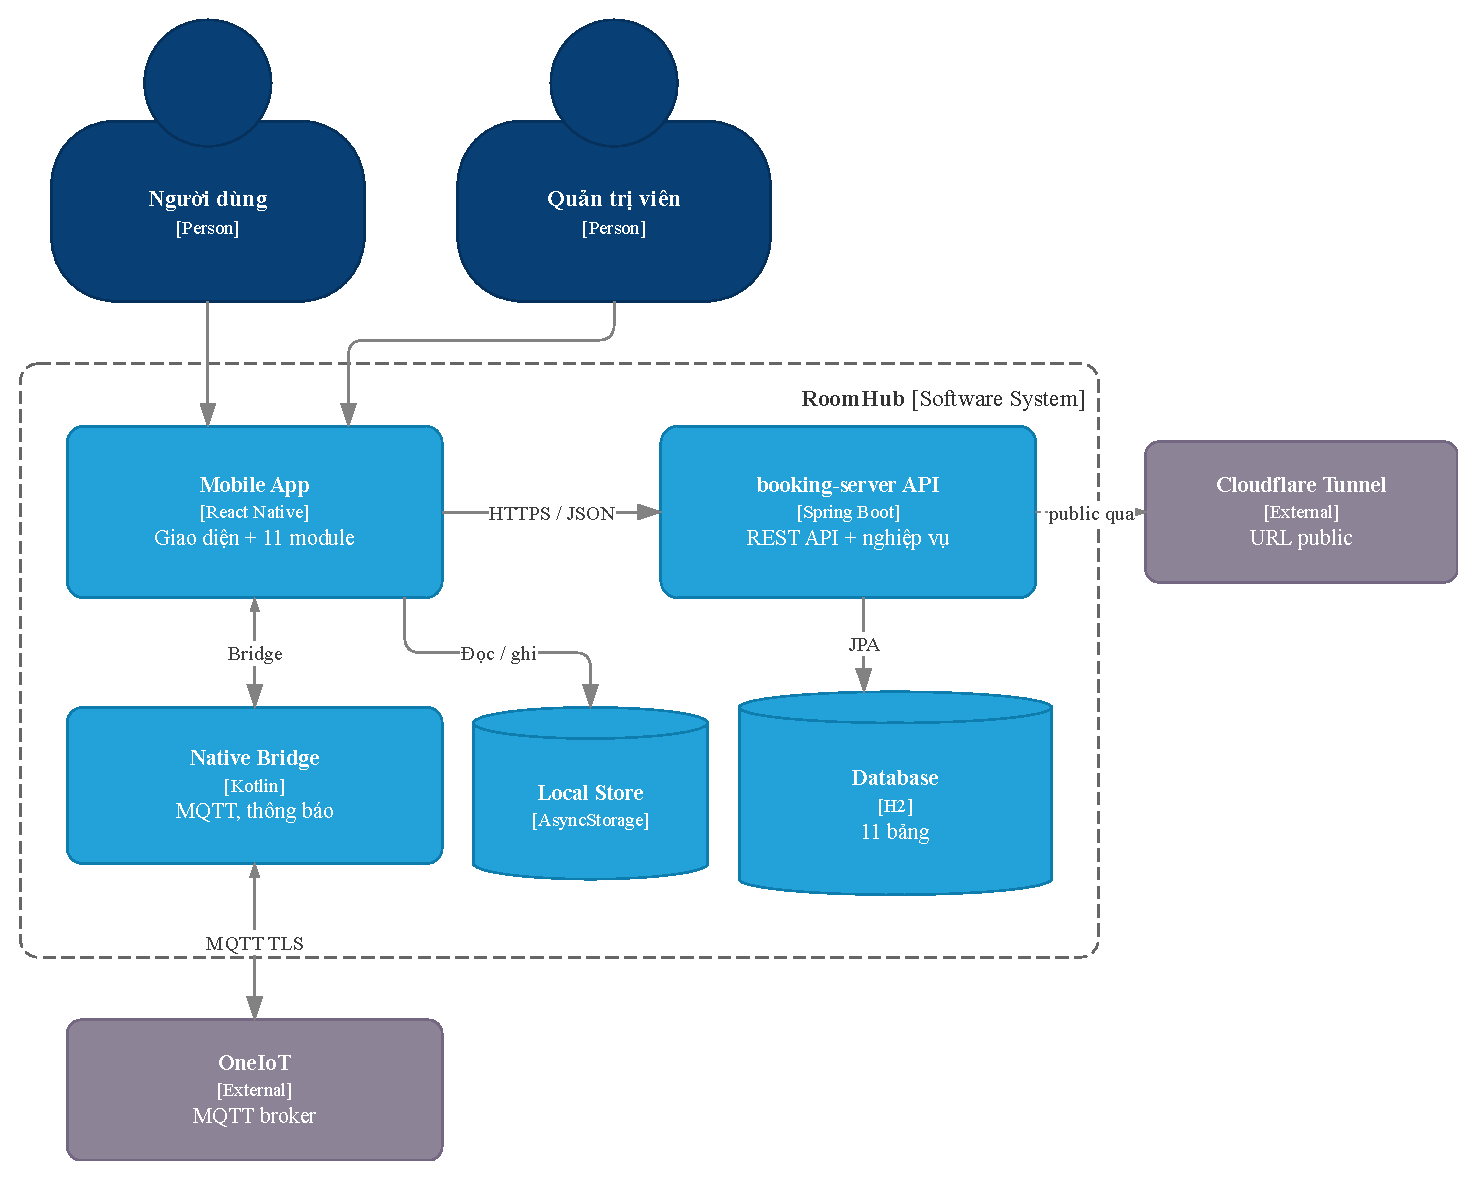
\includegraphics[width=\textwidth,height=.76\textheight,keepaspectratio]{Hinhve/design/10_c4_l2_container.pdf}
\caption{Các thành phần chạy: app Android, REST backend và OneIoT}\label{fig:containers}
\end{figure}

Luồng local là UI → repository → readJson/writeJson → Async Storage. Luồng remote là UI → apiRequest → SessionAuthFilter → controller theo nghiệp vụ → BookingService → JPA/H2. Luồng khóa là service TypeScript → module Kotlin → OneIoT theo MQTT/oneM2M. Công tắc REST không bật hoặc tắt kết nối MQTT.

Nguồn local và nguồn REST dùng cùng giao diện nghiệp vụ ở màn hình nhưng là hai kho độc lập. Chế độ REST không tự lấy backlog local, không tự hòa giải dữ liệu nhiều máy và không tự chuyển về local khi mạng lỗi. Cấu hình bản build quyết định nguồn dữ liệu sử dụng.

\subsection{Module ứng dụng và trách nhiệm lớp phía server}
Hình~\ref{fig:app-components} bổ sung cách các module cộng tác; Hình~\ref{fig:server-components} cho biết ranh giới HTTP, xác thực, nghiệp vụ và dữ liệu ở server. Hai góc nhìn làm rõ phụ thuộc giữa các module trong app và đường xử lý yêu cầu phía Java.
\begin{figure}[H]\centering
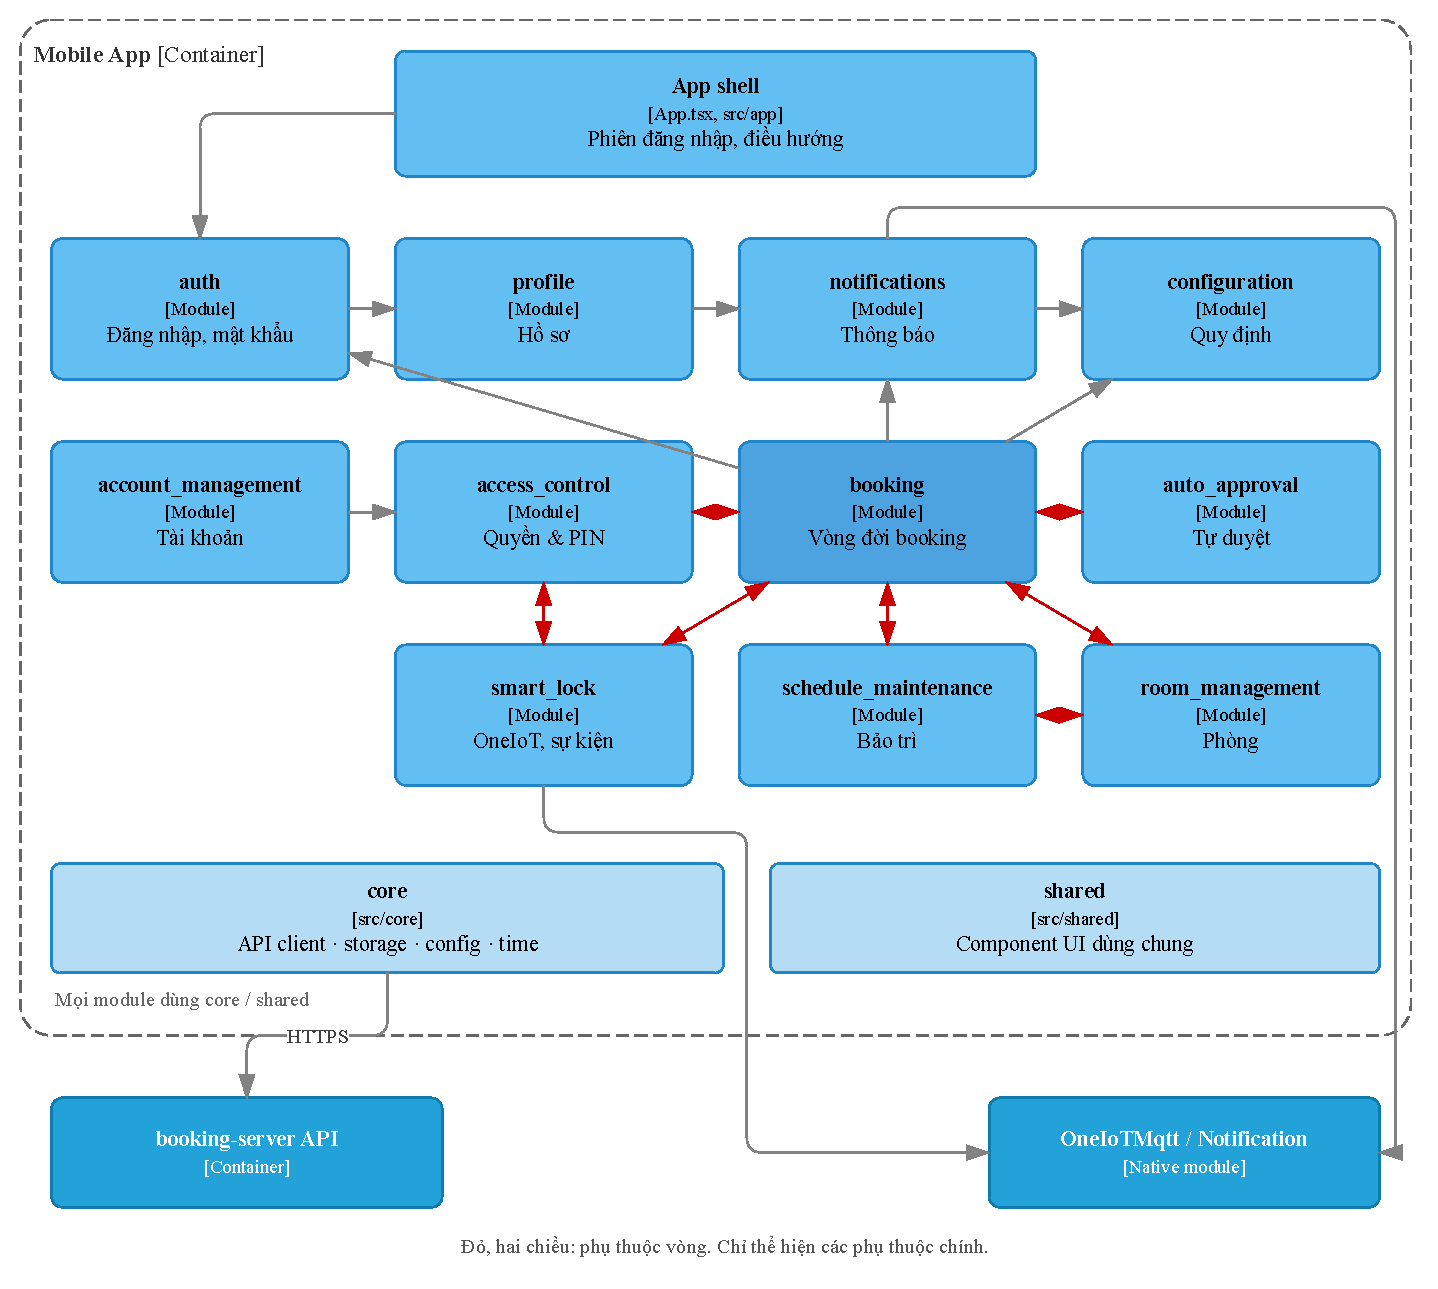
\includegraphics[width=\textwidth,height=.76\textheight,keepaspectratio]{Hinhve/design/11a_c4_l3_component_app.pdf}
\caption{Trách nhiệm và các phụ thuộc chính giữa module React Native}\label{fig:app-components}
\end{figure}
\begin{figure}[H]\centering
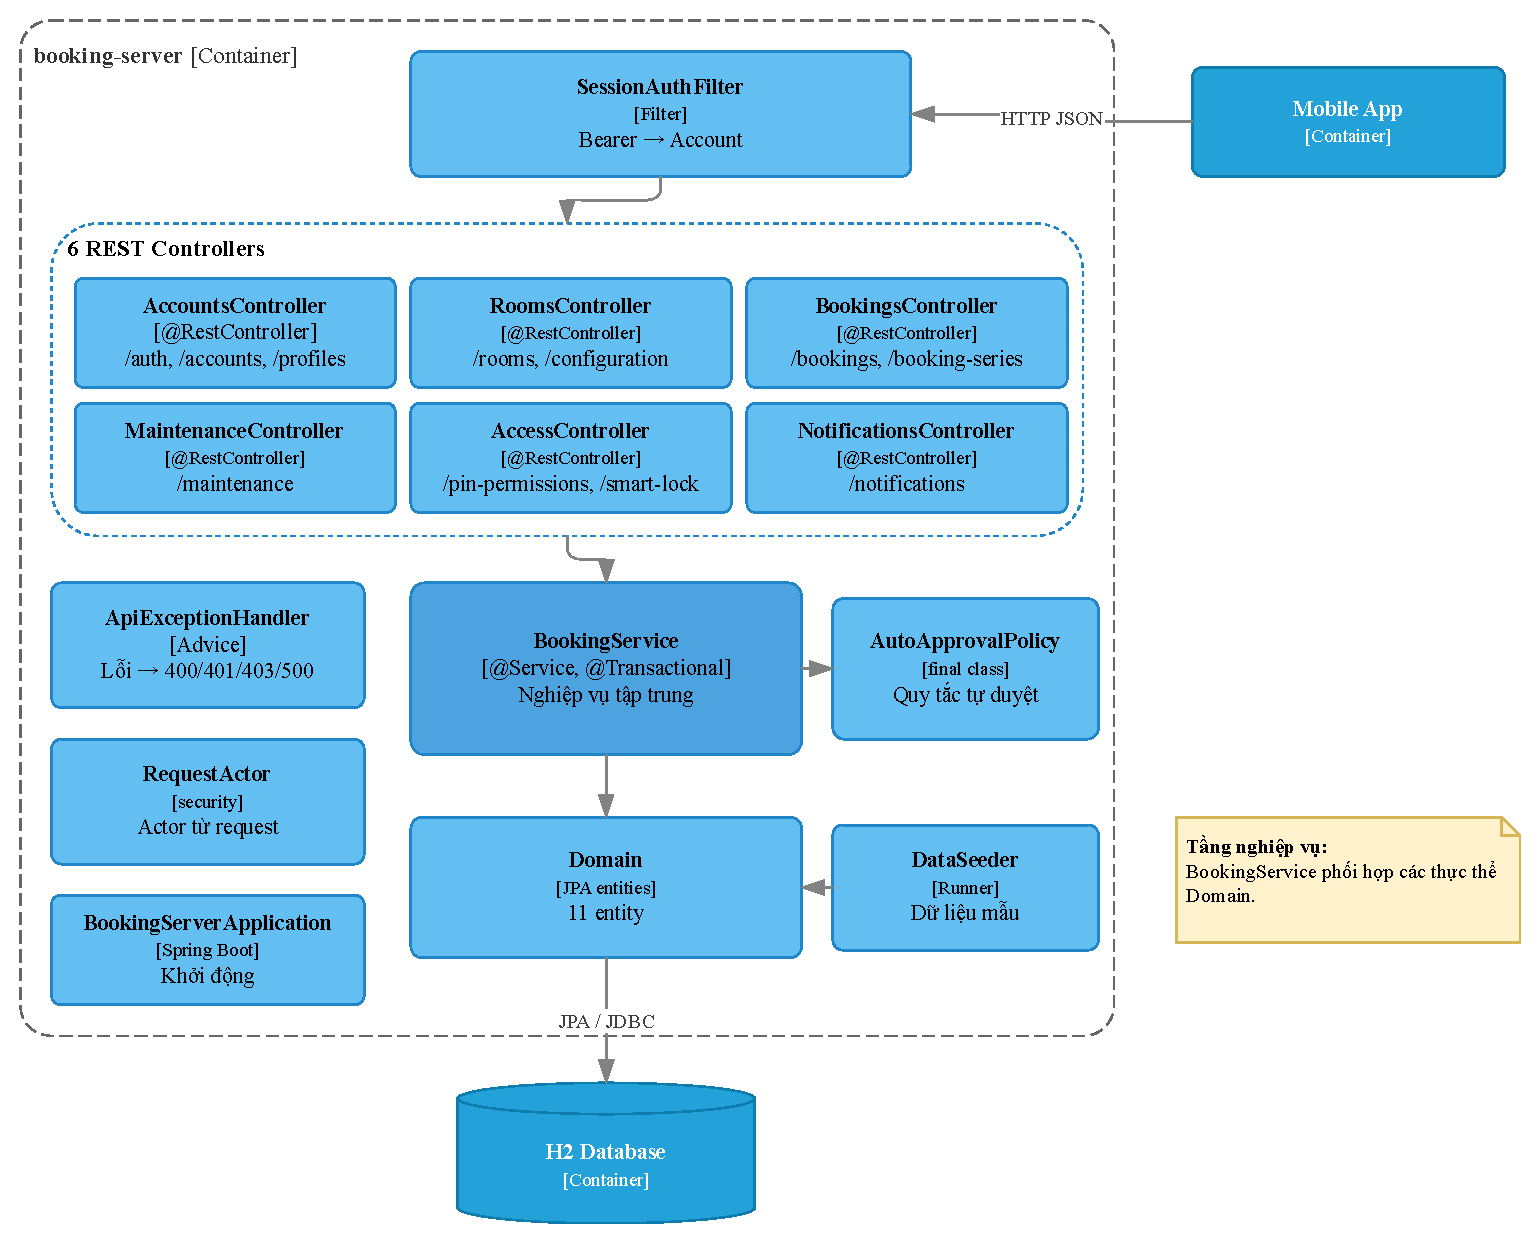
\includegraphics[width=\textwidth,height=.76\textheight,keepaspectratio]{Hinhve/design/12_c4_l3_component_server.pdf}
\caption{Các lớp giao tiếp, nghiệp vụ và lưu trữ của backend}\label{fig:server-components}
\end{figure}

\FloatBarrier
{\tabletext\renewcommand{\arraystretch}{1.04}\begin{longtable}{>{\raggedright\arraybackslash}p{\dimexpr0.28\textwidth-2\tabcolsep\relax}>{\raggedright\arraybackslash}p{\dimexpr0.72\textwidth-2\tabcolsep\relax}}
\caption{Trách nhiệm của 11 module nghiệp vụ}\label{tab:design-modules}\\
\toprule \textbf{Module} & \textbf{Trách nhiệm và cộng tác}\\\midrule
\endfirsthead
\multicolumn{2}{l}{\small Trách nhiệm của 11 module nghiệp vụ (tiếp)}\\
\toprule \textbf{Module} & \textbf{Trách nhiệm và cộng tác}\\\midrule
\endhead
\bottomrule\endlastfoot
\code{auth} & Đăng ký/đăng nhập, mật khẩu và xác thực vai trò; tài khoản quản trị cũng dùng accountRepository.\\\addlinespace[1.5pt]
\code{account_management} & UI quản lý tài khoản và quyền PIN; gọi auth và access control.\\\addlinespace[1.5pt]
\code{room_management} & Danh mục, bộ lọc và sơ đồ tầng; màn tìm và đặt gọi nghiệp vụ booking. Quản lý phòng ghép với bảo trì.\\\addlinespace[1.5pt]
\code{booking} & Tạo, duyệt, lịch lặp, hủy/đổi phòng, nhận chìa, ủy quyền, ghi chú và no-show; dùng phòng, cấu hình, bảo trì, tự duyệt và thông báo.\\\addlinespace[1.5pt]
\code{auto_approval} & Tính quyết định duyệt từ cấu hình và dấu phòng đặc biệt sau khi yêu cầu đã qua validation.\\\addlinespace[1.5pt]
\code{access_control} & Quyền theo user--phòng; tạo và lưu PIN theo booking đã duyệt, gọi smart lock khi có thể gửi.\\\addlinespace[1.5pt]
\code{smart_lock} & Quản lý một khóa gắn phòng; cấp password ID, kết nối native OneIoT và tiếp nhận sự kiện.\\\addlinespace[1.5pt]
\code{schedule_maintenance} & Yêu cầu bảo trì, lịch đã được admin lên và kiểm xung đột.\\\addlinespace[1.5pt]
\code{configuration} & Cửa sổ đặt trước, hạn mức, các thời hạn và công tắc tự duyệt/thông báo.\\\addlinespace[1.5pt]
\code{profile} & Hồ sơ người dùng theo tài khoản.\\\addlinespace[1.5pt]
\code{notifications} & Lưu/đọc theo người nhận, banner và cầu thông báo native; chỉ hiện banner cho tài khoản đang đăng nhập.\\\addlinespace[1.5pt]
\end{longtable}}

Lớp hạ tầng dùng chung cung cấp HTTP client, lưu trữ JSON, cấu hình và xử lý thời gian; lớp giao diện dùng chung cung cấp các thành phần tái sử dụng. Các module cộng tác qua service và hợp đồng dữ liệu, trong đó nghiệp vụ đặt phòng phối hợp với cấu hình, bảo trì, cấp quyền và thông báo.

{\tabletext\renewcommand{\arraystretch}{1.04}\begin{longtable}{>{\raggedright\arraybackslash}p{\dimexpr0.31\textwidth-2\tabcolsep\relax}>{\raggedright\arraybackslash}p{\dimexpr0.69\textwidth-2\tabcolsep\relax}}
\caption{Trách nhiệm các lớp Java và dữ liệu trao đổi}\label{tab:server-responsibilities}\\
\toprule \textbf{Nhóm lớp} & \textbf{Trách nhiệm đã triển khai}\\\midrule
\endfirsthead
\multicolumn{2}{l}{\small Trách nhiệm các lớp Java và dữ liệu trao đổi (tiếp)}\\
\toprule \textbf{Nhóm lớp} & \textbf{Trách nhiệm đã triển khai}\\\midrule
\endhead
\bottomrule\endlastfoot
\code{BookingServerApplication}, \code{DataSeeder} & Khởi động dịch vụ và bổ sung dữ liệu trình diễn, không đại diện cơ sở vật chất thực tế.\\\addlinespace[1.5pt]
\code{SessionAuthFilter}, \code{RequestActor} & Tra token Bearer thành tài khoản, đặt actor trong request và cung cấp actor cho controller.\\\addlinespace[1.5pt]
Sáu controller & Nhận route/body, chuyển actor và dữ liệu tới service, tạo phản hồi HTTP. Các controller dùng chung lớp BookingService.\\\addlinespace[1.5pt]
\code{BookingService} & Xác thực/quyền, các nghiệp vụ và giao dịch; dùng EntityManager để truy vấn, khóa và ghi dữ liệu.\\\addlinespace[1.5pt]
\code{AutoApprovalPolicy} & Quy tắc tự duyệt dùng chung ở luồng tạo booking phía server.\\\addlinespace[1.5pt]
\code{Domain} và converter & 11 entity, cấu trúc nhúng, chuyển danh sách/đối tượng lồng thành JSON.\\\addlinespace[1.5pt]
Record đầu vào/kết quả & Hợp đồng request/response cho phòng, booking, PIN, cấu hình liên quan; tách dữ liệu trao đổi khỏi tham số HTTP.\\\addlinespace[1.5pt]
\code{ApiExceptionHandler} & Chuyển lỗi dữ liệu thành 400, phiên thành 401, quyền thành 403 và lỗi còn lại thành 500, kèm thông điệp JSON.\\\addlinespace[1.5pt]
\end{longtable}}

\subsection{Triển khai trên điện thoại và các kết nối}
Hình~\ref{fig:deployment} mô tả bố trí triển khai: APK/bundle/native chạy trên Android; Java/H2 chạy trên máy chủ; kết nối OneIoT đi từ app tới broker. Metro và ADB phục vụ phát triển hoặc kết nối thử; bản Release local không cần Metro để khởi chạy. Cloudflare và H2 SSL là lựa chọn môi trường, không phải thành phần bắt buộc của bản local.
\begin{figure}[H]\centering
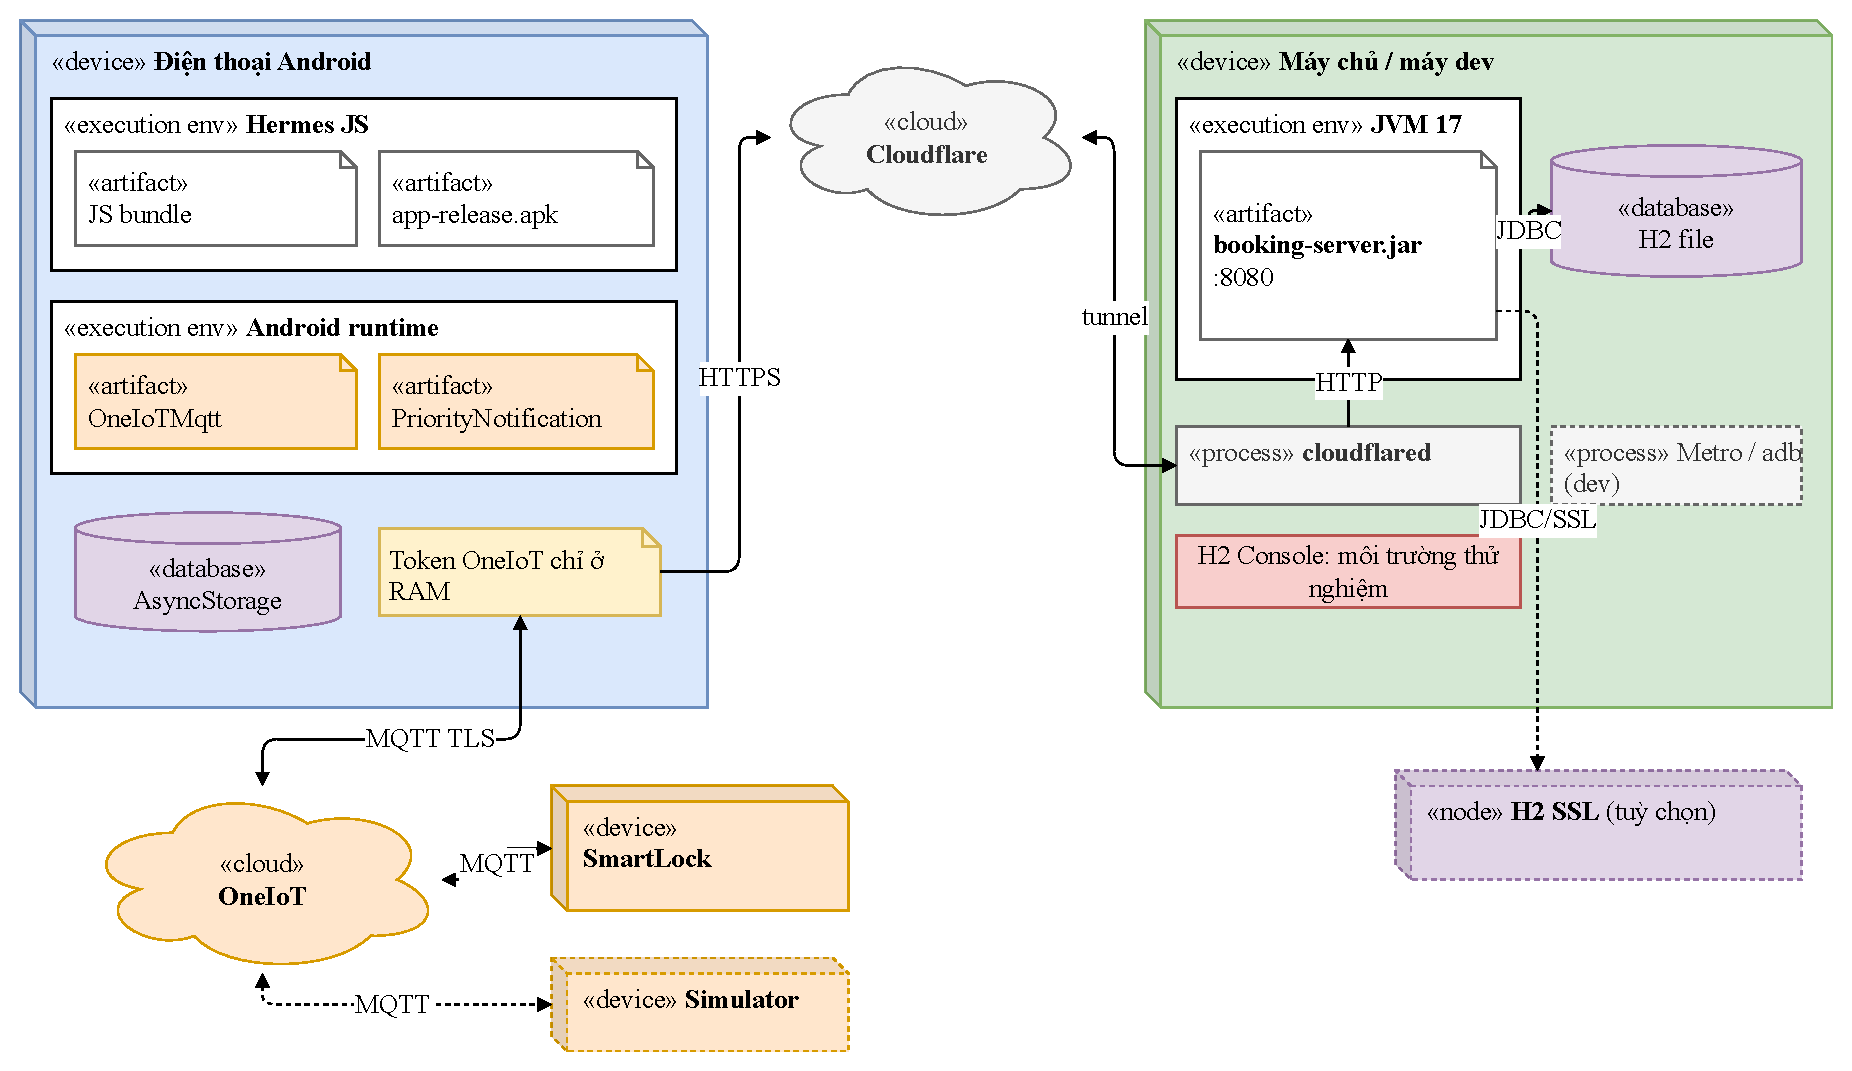
\includegraphics[width=\textwidth,height=.76\textheight,keepaspectratio]{Hinhve/design/14_deployment_diagram.pdf}
\caption{Bố trí triển khai ứng dụng Android, backend và kết nối SmartLock}\label{fig:deployment}
\end{figure}

Ứng dụng Android kết nối trực tiếp OneIoT qua native MQTT để gửi lệnh và tiếp nhận sự kiện từ SmartLock. Backend cung cấp dữ liệu nghiệp vụ qua REST khi bật chế độ remote; chế độ local lưu dữ liệu trên thiết bị. Simulator và gateway là các chương trình hỗ trợ riêng. Các thành phần app và SmartLock đã được nhóm triển khai, chạy thử và hoàn thành các chức năng thực tế.

\FloatBarrier
\section{Mô hình dữ liệu và giao tiếp dịch vụ}
\subsection{Thực thể, thuộc tính và quan hệ logic}
Mô hình dữ liệu gồm tài khoản, tài nguyên phòng và các bản ghi sử dụng, tiếp cận, bảo trì. Các thực thể liên hệ bằng định danh chuỗi; Bảng~\ref{tab:data} tổng hợp thuộc tính và quan hệ chính. Lược đồ ER chi tiết nằm ở Phụ lục~\ref{app:evidence}.
{\tabletext\renewcommand{\arraystretch}{1.04}\begin{longtable}{>{\raggedright\arraybackslash}p{\dimexpr0.27\textwidth-2\tabcolsep\relax}>{\raggedright\arraybackslash}p{\dimexpr0.39\textwidth-2\tabcolsep\relax}>{\raggedright\arraybackslash}p{\dimexpr0.34\textwidth-2\tabcolsep\relax}}
\caption{Mười một thực thể và quan hệ nghiệp vụ chính}\label{tab:data}\\
\toprule \textbf{Thực thể / bảng} & \textbf{Thuộc tính chính} & \textbf{Liên hệ và điều kiện}\\\midrule
\endfirsthead
\multicolumn{3}{l}{\small Mười một thực thể và quan hệ nghiệp vụ chính (tiếp)}\\
\toprule \textbf{Thực thể / bảng} & \textbf{Thuộc tính chính} & \textbf{Liên hệ và điều kiện}\\\midrule
\endhead
\bottomrule\endlastfoot
Account / accounts & username, password, recoveryCode, role, active. & Username là định danh; trạng thái và vai trò quyết định đăng nhập/quyền.\\\addlinespace[1.5pt]
Profile / user\_profiles & username, thông tin họ tên, liên hệ, đơn vị. & Hồ sơ theo tài khoản; user không sửa hồ sơ người khác qua API.\\\addlinespace[1.5pt]
AuthSession / auth\_sessions & token, username, createdAt. & Server tra token để nhận diện actor, không tin username do client tự gửi.\\\addlinespace[1.5pt]
Room / rooms & id, name, floor, capacity, equipment, lockType, status, requiresApproval. & Một phòng có nhiều booking/bảo trì theo thời gian; dấu đặc biệt làm phòng luôn cần admin duyệt.\\\addlinespace[1.5pt]
Booking / bookings & requesterUsername, roomId, date/start/end, purpose, status, metadata duyệt và chuỗi lặp. & Tâm điểm liên kết tài khoản, phòng, PIN, nhận chìa, sự kiện, đổi phòng và yêu cầu bảo trì.\\\addlinespace[1.5pt]
PinPermission / pin\_permissions & username, roomId, active, thông tin cấp/thu hồi. & Quyền cho một cặp tài khoản--phòng, tách khỏi vai trò admin và vẫn phải kiểm booking.\\\addlinespace[1.5pt]
ManagedSmartLock / managed\_smart\_locks & assignedRoomId, thông tin khóa/kết nối, nextPasswordId. & Một khóa quản lý gắn tối đa một phòng PIN; password ID quay vòng 1--255.\\\addlinespace[1.5pt]
Maintenance / maintenance\_records & roomId, date/start/end, reason, cancelledAt. & Lịch hiệu lực chặn khoảng phòng; hủy lịch không xóa lịch sử.\\\addlinespace[1.5pt]
MaintenanceRequest / maintenance\_requests & bookingId, roomId, requesterUsername, reason, status, maintenanceRecordId. & Yêu cầu chờ xử lý khác lịch đã được admin lên.\\\addlinespace[1.5pt]
Notification / notifications & username, title, message, createdAt, read. & Đọc/đánh dấu theo người nhận của phiên.\\\addlinespace[1.5pt]
Configuration / app\_configuration & Cửa sổ ngày, hạn mức, các cutoff/grace, tự duyệt và thông báo. & Bản ghi cấu hình chung được đọc ở các bước kiểm nghiệp vụ.\\\addlinespace[1.5pt]
\end{longtable}}

PIN tạm được nhúng trong Booking bằng \code{@Embedded}; thông tin hẹn/đề xuất nhận chìa, ủy quyền, đổi phòng và danh sách sự kiện dùng cấu trúc lồng hoặc converter JSON. Các quan hệ trên ERD biểu diễn tham chiếu logic theo định danh; tính hợp lệ của các liên hệ được kiểm ở tầng nghiệp vụ, thay cho ánh xạ toàn bộ bằng quan hệ đối tượng JPA.

Dữ liệu thời gian trao đổi gồm ngày dạng YYYY-MM-DD, giờ HH:mm và các mốc ISO/epoch tùy trường. Service Java dùng múi giờ Việt Nam khi kiểm nghiệp vụ, còn local dựng thời điểm theo thiết bị. Đồng hồ và múi giờ ảnh hưởng trực tiếp đến đặt cùng ngày, no-show và khoảng hiệu lực PIN.

\subsection{Hợp đồng REST và xử lý lỗi}
Giao tiếp REST được tổ chức theo sáu controller nghiệp vụ. Các nhóm API bao gồm tài khoản, phòng, booking, lịch lặp, quyền truy cập, nhận chìa, điểm danh, bảo trì và thông báo. Bảng~\ref{tab:api-design} tổng hợp 51 cặp phương thức/đường dẫn thành 20 nhóm thao tác.
{\tabletext\renewcommand{\arraystretch}{1.04}\begin{longtable}{>{\raggedright\arraybackslash}p{\dimexpr0.49\textwidth-2\tabcolsep\relax}>{\raggedright\arraybackslash}p{\dimexpr0.51\textwidth-2\tabcolsep\relax}}
\caption{Tổng hợp endpoint, dữ liệu và quyền truy cập}\label{tab:api-design}\\
\toprule \textbf{Phương thức / đường dẫn} & \textbf{Dữ liệu và kiểm soát}\\\midrule
\endfirsthead
\multicolumn{2}{l}{\small Tổng hợp endpoint, dữ liệu và quyền truy cập (tiếp)}\\
\toprule \textbf{Phương thức / đường dẫn} & \textbf{Dữ liệu và kiểm soát}\\\midrule
\endhead
\bottomrule\endlastfoot
\code{POST /api/auth/login}; \code{POST /api/auth/register} & Login nhận username/password, trả token/username/role. Đăng ký kiểm dữ liệu và trả phiên; không cần token trước.\\\addlinespace[1.5pt]
\code{POST /api/auth/change-password}; \code{POST /api/auth/reset-password} & Đổi mật khẩu dùng actor/mật khẩu hiện tại; reset dùng username/mã khôi phục. Reset là ngoại lệ không bắt token tại filter.\\\addlinespace[1.5pt]
\code{GET,POST /api/accounts}; \code{PUT,DELETE /api/accounts/{username}} & Admin quản lý tài khoản; service chặn các thao tác vi phạm quyền hoặc điều kiện dữ liệu đang dùng.\\\addlinespace[1.5pt]
\code{GET,PUT /api/profiles/{username}} & Hồ sơ gắn tài khoản; service kiểm quyền truy cập theo actor.\\\addlinespace[1.5pt]
\code{GET,POST /api/rooms}; \code{PUT,DELETE /api/rooms/{id}} & Danh sách cho phiên hợp lệ; ghi phòng cần admin, kiểm tên/tầng/sức chứa/loại khóa.\\\addlinespace[1.5pt]
\code{GET,PUT /api/configuration} & Đọc quy tắc; admin ghi. Client cũ bỏ qua trường mới không làm mất giá trị hiện có theo code xử lý.\\\addlinespace[1.5pt]
\code{GET /api/room-occupancy} & Trả các khoảng sử dụng để tính trạng thái phòng theo lịch, không chỉ theo cờ AVAILABLE.\\\addlinespace[1.5pt]
\code{GET,POST /api/bookings} & Đọc theo phạm vi tài khoản; tạo nhận phòng/ngày/giờ/mục đích/lặp, kiểm role và quy tắc trước ghi.\\\addlinespace[1.5pt]
\code{POST /api/bookings/{id}/review}; \code{POST /api/bookings/{id}/change-room} & Admin duyệt/từ chối hoặc đổi phòng; kiểm trạng thái, quyền và điều kiện áp dụng.\\\addlinespace[1.5pt]
\code{POST /api/bookings/{id}/cancel} & User chủ lượt; kiểm trạng thái/thời hạn, chuyển CANCELLED và đánh dấu PIN thu hồi trong dữ liệu; không xóa quyền phòng toàn cục.\\\addlinespace[1.5pt]
\code{POST /api/booking-series/{seriesId}/review}; \code{PUT /api/booking-series/{seriesId}/pending}; \code{POST /api/booking-series/{seriesId}/cancel} & Xử lý các lượt trong chuỗi theo trạng thái; không xem thao tác chuỗi là quyền bỏ qua xung đột từng lượt.\\\addlinespace[1.5pt]
\code{GET,POST /api/pin-permissions}; \code{POST /api/pin-permissions/revoke} & Đọc/cấp/thu hồi quyền theo user--phòng; thao tác quản trị kiểm role trong service.\\\addlinespace[1.5pt]
\code{POST /api/bookings/{id}/temporary-pin} & Lưu/cập nhật mã, khoảng hiệu lực và trạng thái gửi; kiểm chủ lượt/admin, booking đã duyệt và quyền liên quan.\\\addlinespace[1.5pt]
\code{GET /api/smart-lock}; \code{POST /api/smart-lock/assign}; \code{POST /api/smart-lock/unassign}; \code{POST /api/smart-lock/reserve-password-id} & Quản lý khóa/phòng và cấp ID; cấp ID kiểm phòng khớp, khóa dữ liệu và quyền user nếu actor không phải admin.\\\addlinespace[1.5pt]
\code{POST /api/bookings/{id}/pickup/propose}; \code{POST /api/bookings/{id}/pickup/schedule}; \code{POST /api/bookings/{id}/pickup/accept}; \code{PUT /api/bookings/{id}/delegate} & Trao đổi thời gian/địa điểm nhận chìa và người nhận hộ; service kiểm quyền và thứ tự trạng thái thương lượng.\\\addlinespace[1.5pt]
\code{POST /api/bookings/access-event}; \code{POST /api/bookings/{id}/check-in}; \code{POST /api/bookings/{id}/no-show} & Ghi sự kiện khóa hoặc xác nhận điểm danh theo quyền; kiểm thời gian và bằng chứng có mặt/no-show.\\\addlinespace[1.5pt]
\code{GET,POST /api/maintenance}; \code{POST /api/maintenance/{id}/cancel} & Đọc/lập/hủy lịch bảo trì; lập lịch cần admin và kiểm xung đột.\\\addlinespace[1.5pt]
\code{GET,POST /api/maintenance/requests}; \code{POST /api/maintenance/requests/{id}/schedule}; \code{POST /api/maintenance/requests/{id}/reject} & Yêu cầu từ booking đang dùng, được admin lên lịch hoặc từ chối.\\\addlinespace[1.5pt]
\code{POST /api/bookings/{id}/room-observation} & Gửi ghi chú cho admin, không tự tạo yêu cầu hoặc lịch bảo trì.\\\addlinespace[1.5pt]
\code{GET,POST /api/notifications}; \code{POST /api/notifications/read} & Đọc/đánh dấu theo phiên; tạo thông báo còn phải qua kiểm tra quyền service.\\\addlinespace[1.5pt]
\end{longtable}}

\code{SessionAuthFilter} bỏ qua ba route login/register/reset-password; các route API còn lại cần token Bearer hợp lệ. User không được chọn username người khác để mở rộng dữ liệu trả về. Client bọc fetch, thêm Authorization, xử lý JSON/204/401 và timeout 12 giây; API lỗi dùng trường \textit{\{message\}}. Kết quả kiểm thử API và tích hợp được trình bày ở Chương~\ref{chap:testing}.

\FloatBarrier
\section{Thiết kế giao diện và điều hướng}
\subsection{Luồng màn hình theo vai trò}
Giao diện Android dọc dùng dashboard, đầu trang, Back, chuông và menu tài khoản. Tìm phòng theo tầng/ngày/giờ và gửi yêu cầu trên cùng màn hình. Hình~\ref{fig:flow-user}--\ref{fig:flow-admin} mô tả điều hướng hai vai trò; ảnh thực nghiệm ở Chương~\ref{chap:implementation}.
\begin{figure}[H]\centering
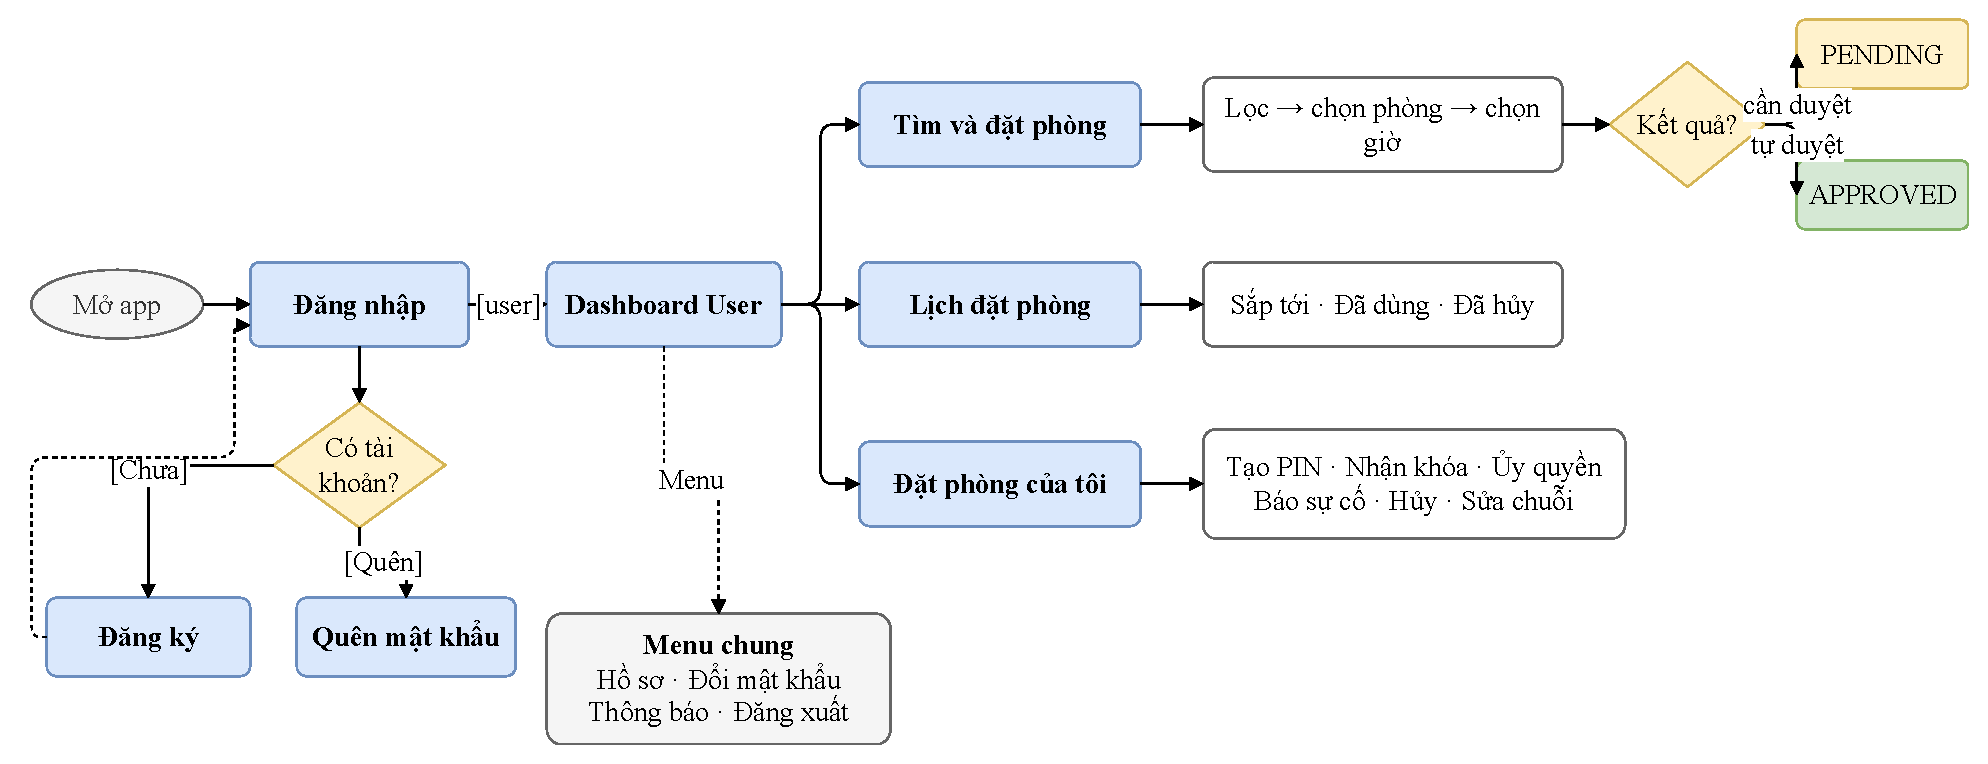
\includegraphics[width=\textwidth,height=.76\textheight,keepaspectratio]{Hinhve/design/05a_user_flow_nguoi_dung.pdf}
\caption{Luồng màn hình và các tác vụ chính của người dùng}\label{fig:flow-user}
\end{figure}
\begin{figure}[H]\centering
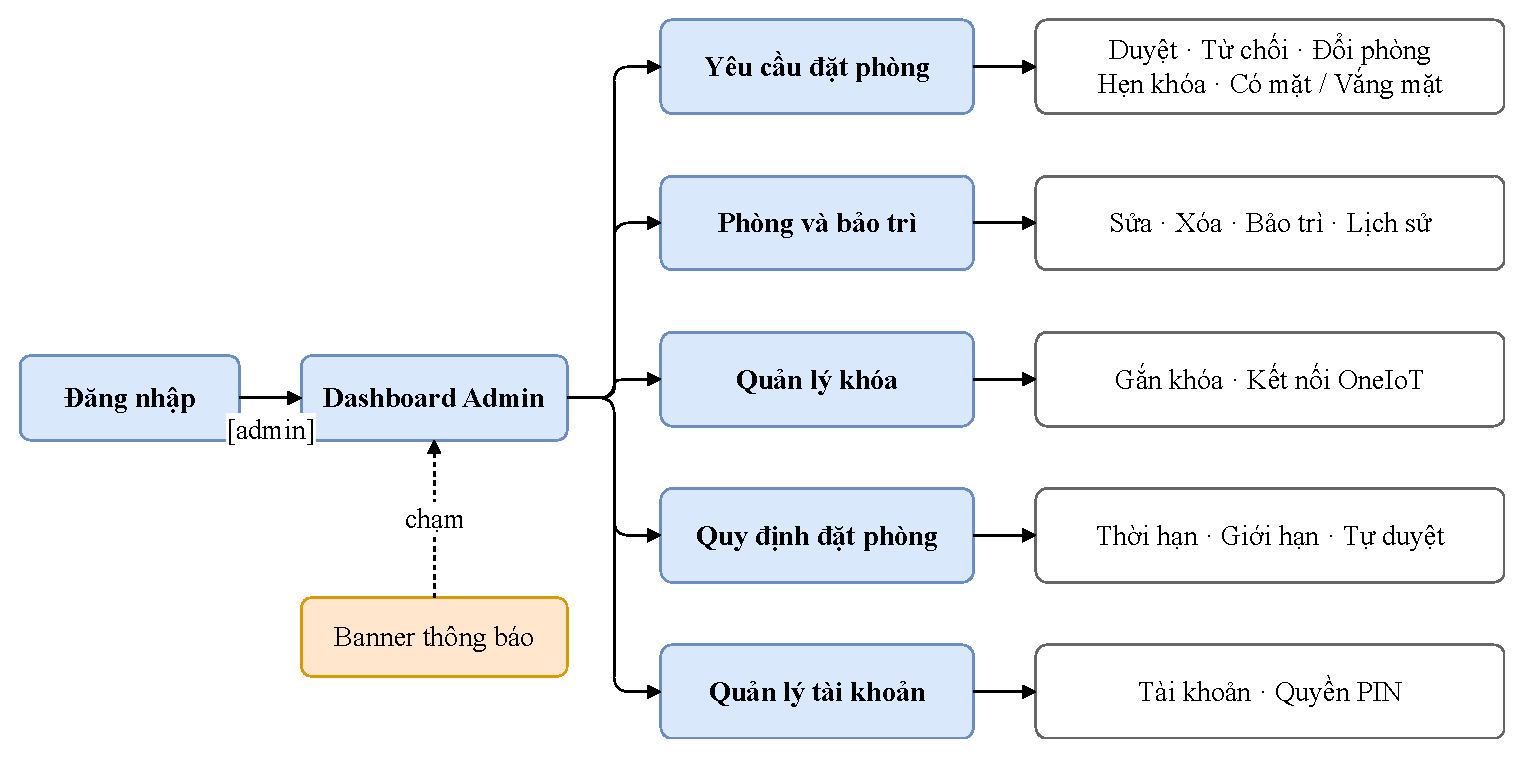
\includegraphics[width=\textwidth,height=.76\textheight,keepaspectratio]{Hinhve/design/05b_user_flow_quan_tri_vien.pdf}
\caption{Luồng màn hình quản trị và các điểm vào từ thông báo}\label{fig:flow-admin}
\end{figure}

\FloatBarrier
{\tabletext\renewcommand{\arraystretch}{1.04}\begin{longtable}{>{\raggedright\arraybackslash}p{\dimexpr0.31\textwidth-2\tabcolsep\relax}>{\raggedright\arraybackslash}p{\dimexpr0.69\textwidth-2\tabcolsep\relax}}
\caption{Màn hình, mục đích và dữ liệu điều hướng}\label{tab:navigation}\\
\toprule \textbf{Điểm vào} & \textbf{Trách nhiệm / tham số}\\\midrule
\endfirsthead
\multicolumn{2}{l}{\small Màn hình, mục đích và dữ liệu điều hướng (tiếp)}\\
\toprule \textbf{Điểm vào} & \textbf{Trách nhiệm / tham số}\\\midrule
\endhead
\bottomrule\endlastfoot
Đăng nhập, đăng ký, khôi phục mật khẩu & Chọn form xác thực qua selectedFeature trong LoginScreen; khi đăng nhập thành công, callback chuyển session lên App.\\\addlinespace[1.5pt]
Dashboard User & Mở Tìm và đặt phòng, Lịch đặt phòng, Đặt phòng của tôi; truyền username và onBack cho màn con.\\\addlinespace[1.5pt]
Dashboard Admin & Mở Yêu cầu đặt phòng, Quản lý tài khoản, Quản lý phòng và bảo trì, Quản lý khóa, Quy định đặt phòng; truyền thông tin admin khi cần.\\\addlinespace[1.5pt]
Menu tài khoản và chuông & Mở hồ sơ, đổi mật khẩu, thông báo; logout xóa phiên trong UI. Banner/notification có thể đưa admin tới màn xử lý yêu cầu.\\\addlinespace[1.5pt]
Đặt phòng của tôi & Phân nhóm lượt theo thời gian/trạng thái; mở thao tác sửa/hủy chuỗi, PIN, nhận chìa, ủy quyền và phản ánh phòng.\\\addlinespace[1.5pt]
Quản lý phòng và bảo trì & Chọn tầng/phòng; chỉnh thông tin, xem lịch hoặc lập/xử lý bảo trì trên cùng màn hình.\\\addlinespace[1.5pt]
\end{longtable}}

\subsection{Cơ chế chuyển màn, làm mới và quay lại}
Bảng điều khiển dùng trạng thái \code{activeScreen} để chọn màn hình hiển thị. Props mang dữ liệu và callback thay route params. Khi đóng màn con, \code{closeChildScreen} đặt màn đang chọn về null rồi làm mới số thông báo/yêu cầu. BackHandler đóng menu trước, sau đó quay về dashboard; listener được tháo khi effect thay đổi hoặc unmount.

App yêu cầu đăng nhập lại khi khởi động; các màn hình được điều khiển bằng state và callback. Loading/error và cleanup listener/timer là trách nhiệm từng luồng bất đồng bộ.

\FloatBarrier
\section{Dữ liệu cá nhân, quyền thiết bị và các ràng buộc}
AndroidManifest khai báo INTERNET, POST\_NOTIFICATIONS và VIBRATE. Trên Android từ API 33, app kiểm và xin quyền thông báo khi chạy \cite{android}; từ chối quyền không đồng nghĩa nghiệp vụ đặt phòng bị cấm, nhưng thông báo hệ điều hành có thể không hiện. Ứng dụng không xin quyền vị trí, camera hoặc micro cho luồng đặt phòng hiện tại.

Token REST và OneIoT giữ trong RAM của phiên. Token OneIoT không được ghi vào source hoặc Async Storage; app ngắt MQTT khi đăng xuất hoặc xuống nền, việc nhận sự kiện khóa diễn ra trong phiên MQTT đang hoạt động. Mật khẩu/PIN và một phần dữ liệu khôi phục hiện còn dạng rõ trong local/entity server. Mã hóa gói lệnh khóa không giải quyết việc bảo vệ các dữ liệu lưu này.

Native TLS đang bỏ qua xác minh chứng thư; Android cho phép cleartext để thử HTTP. Hướng gia cố bảo mật gồm xác thực, bảo vệ lưu trữ, chứng thư và phân quyền khi mở rộng triển khai. H2 console và đường tunnel trong sơ đồ là cấu hình thử nghiệm cần quản lý theo môi trường. Chế độ local dùng được khi thiếu backend, nhưng đó là chế độ chọn trước khi build, không phải cơ chế tự fallback/offline sync của REST.

\FloatBarrier
\section{Các giải pháp kỹ thuật cho luồng nghiệp vụ cốt lõi}
Ba nhóm giải pháp tập trung vào tính nhất quán lịch, quyền tiếp cận và tổ chức dữ liệu. Chúng giải thích cách các bước kiểm tra, trạng thái và ranh giới dữ liệu hỗ trợ luồng nghiệp vụ cốt lõi.

\subsection{Chống trùng lịch, giao dịch và quyết định duyệt}
\label{sec:overlap-solution}
\paragraph{Bài toán.} Hai lượt đặt có thể không trùng khi đọc riêng nhưng xung đột khi cùng được ghi. Cần phân biệt khoảng chạm biên với khoảng giao nhau; đồng thời kiểm lại phòng khi admin duyệt vì lịch bảo trì hoặc lượt đã duyệt có thể thay đổi trong thời gian chờ.

\paragraph{Phép kiểm khoảng.} Với cùng ngày, hai khoảng nửa mở \textit{[s1,e1)} và \textit{[s2,e2)} giao nhau khi đồng thời có \textit{s1 < e2} và \textit{s2 < e1}. Dùng bất đẳng thức chặt nên 08:00--09:00 và 09:00--10:00 được xem là liền kề. Ngày khác nhau không giao trong phép kiểm này. Dữ liệu thời gian được chuẩn hóa và kiểm tra trước phép so sánh; khoảng có giờ bắt đầu lớn hơn hoặc bằng giờ kết thúc bị từ chối.

Nghiệp vụ đặt phòng và bảo trì dùng chung phép kiểm khoảng; backend thực hiện điều kiện tương ứng trong tầng dịch vụ. Khi tạo, hệ thống xét phòng, lịch của chính user và bảo trì; khi duyệt một lượt đang chờ, code kiểm lại thời gian kết thúc, bảo trì và xung đột với lượt đã duyệt của phòng. Kiểm tra khi tạo bảo đảm yêu cầu hợp lệ; kiểm tra khi duyệt bảo đảm quyết định dựa trên lịch và bảo trì hiện thời.

\paragraph{Thứ tự giao dịch ở backend.} \code{BookingService.createBooking} dùng \code{@Transactional}, khóa Configuration và Room bằng \code{PESSIMISTIC_WRITE} trước khi đọc lịch. Với chuỗi lặp, từng lượt được sinh, kiểm và bổ sung vào tập xét để phát hiện cả xung đột trong chuỗi (Bảng~\ref{tab:create-transaction}).
{\tabletext\renewcommand{\arraystretch}{1.04}\begin{longtable}{>{\raggedright\arraybackslash}p{\dimexpr0.12\textwidth-2\tabcolsep\relax}>{\raggedright\arraybackslash}p{\dimexpr0.88\textwidth-2\tabcolsep\relax}}
\caption{Thứ tự tạo booking trong giao dịch Java}\label{tab:create-transaction}\\
\toprule \textbf{Bước} & \textbf{Xử lý}\\\midrule
\endfirsthead
\multicolumn{2}{l}{\small Thứ tự tạo booking trong giao dịch Java (tiếp)}\\
\toprule \textbf{Bước} & \textbf{Xử lý}\\\midrule
\endhead
\bottomrule\endlastfoot
1 & Kiểm actor là user và không mạo danh requesterUsername khác.\\\addlinespace[1.5pt]
2 & Khóa cấu hình chung và bản ghi phòng được chọn trước khi đọc lịch.\\\addlinespace[1.5pt]
3 & Kiểm định dạng ngày và số tuần lặp; sinh ngày của từng lượt nếu đặt theo chuỗi.\\\addlinespace[1.5pt]
4 & Validate từng lượt: phòng, giờ, bảo trì, chồng phòng/user, mục đích, cửa sổ và hạn mức theo điều kiện của lượt đầu/lượt lặp.\\\addlinespace[1.5pt]
5 & Tạo booking với trạng thái ban đầu PENDING; lưu metadata chuỗi và bổ sung vào tập đang xét.\\\addlinespace[1.5pt]
6 & Sau validation, AutoApprovalPolicy quyết định có tự duyệt: chỉ khi công tắc bật và phòng không yêu cầu duyệt riêng.\\\addlinespace[1.5pt]
7 & Nhánh tự duyệt cập nhật APPROVED, người duyệt system, quyền PIN nếu phòng PIN và thông báo; nhánh thủ công giữ PENDING và báo admin.\\\addlinespace[1.5pt]
8 & Trả BookingResult trong giao dịch. Lỗi dữ liệu/điều kiện được ném thành ngoại lệ; không trả kết quả thành công cho lượt vi phạm.\\\addlinespace[1.5pt]
\end{longtable}}

\code{reviewBooking} khóa Configuration và booking đích; khi duyệt sẽ kiểm trạng thái PENDING và các điều kiện hiện thời rồi cập nhật quyết định. Quyền PIN được cấp cho phòng khóa số sau khi duyệt. Sơ đồ trình tự Hình~\ref{fig:sequence-booking} bổ sung điểm gọi qua UI, client HTTP, filter, controller và service; thứ tự khóa và kiểm tra dữ liệu được tổng hợp trong Bảng~\ref{tab:create-transaction}.
\begin{figure}[H]\centering
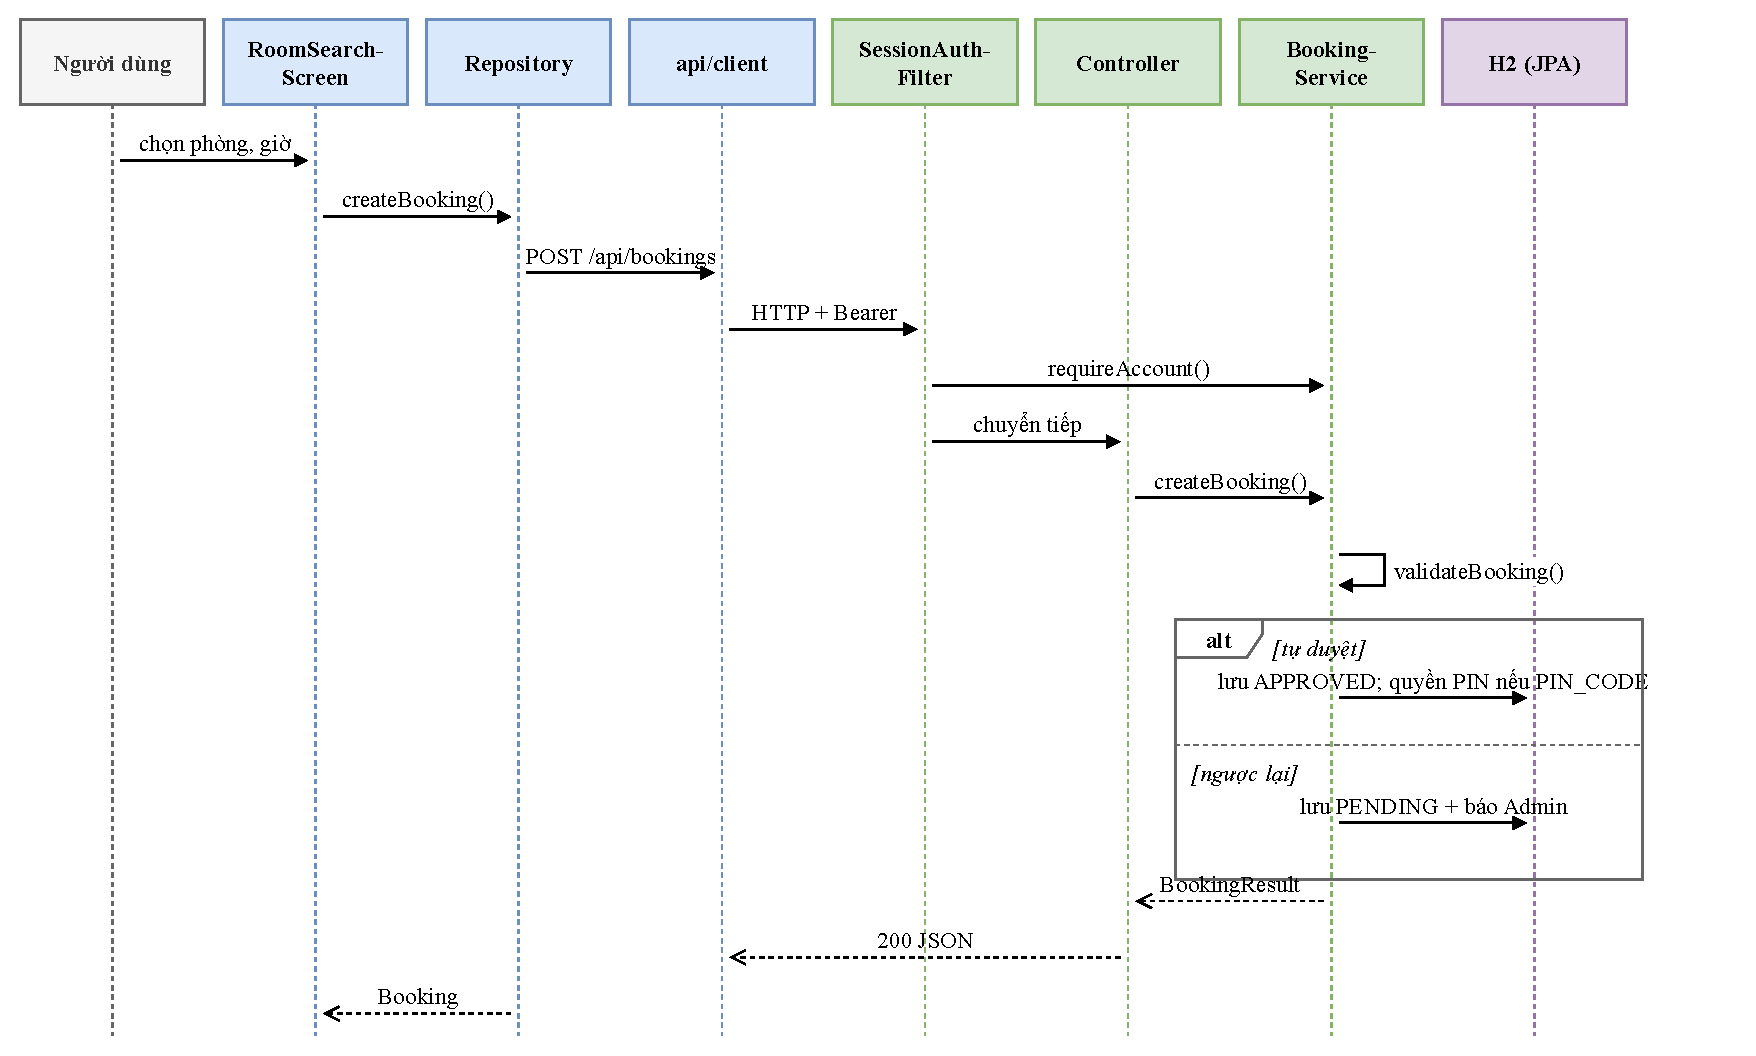
\includegraphics[width=\textwidth,height=.76\textheight,keepaspectratio]{Hinhve/design/15b_sequence_tao_yeu_cau_dat_phong.pdf}
\caption{Trình tự tạo booking qua REST và nhánh tự duyệt/thủ công}\label{fig:sequence-booking}
\end{figure}

\paragraph{Kết quả và hạn chế kỹ thuật.} Các ca kiểm thử ở Chương~\ref{chap:testing} xác nhận xử lý đúng trùng lịch, chạm biên, bảo trì và hạn mức. Backend khóa bản ghi cấu hình/phòng trước khi kiểm và ghi dữ liệu. Khóa cấu hình chung khiến các thao tác dùng cùng tài nguyên phải chờ nhau, là điểm cần tối ưu khi mở rộng. Kho local đọc/ghi JSON, còn backend quản lý giao dịch và khóa dữ liệu bằng JPA.

\FloatBarrier
\subsection{Cấp quyền theo phòng và vòng đời PIN tạm thời}
\label{sec:pin-solution}
\paragraph{Bài toán.} Vai trò user không được biến thành quyền tạo mã ở mọi phòng. Một người chỉ được tạo PIN cho booking đã duyệt của mình, tại phòng được phép và đang gắn khóa phù hợp. Kết nối OneIoT có thể chưa có khi tạo mã, vì vậy lưu mã và gửi lệnh cần là các trạng thái riêng.

\paragraph{Kiểm quyền ở các tầng.} Dịch vụ cấp PIN kiểm vai trò, booking tồn tại/APPROVED, phòng PIN, chủ lượt/quyền theo phòng đối với user, chưa có PIN chưa thu hồi và lượt chưa kết thúc. Admin có quyền thao tác phù hợp nhưng vẫn phải đáp ứng các điều kiện nghiệp vụ của booking/phòng. Khi duyệt tay hoặc tự duyệt phòng PIN, hệ thống cấp quyền cho cặp username--roomId. Thu hồi quyền theo phòng tách khỏi thay đổi role tài khoản.

Mã mới chỉ được tạo khi lượt đặt không còn PIN chưa thu hồi. Do đó, PIN hết thời gian nhưng chưa ghi nhận thu hồi vẫn ngăn việc cấp mã tiếp theo.

\paragraph{Khoảng hiệu lực và ID khóa.} Mã nghiệp vụ có đúng bảy chữ số. Với khoảng sử dụng, validFrom được tính bằng giờ bắt đầu trừ khoảng đệm; validUntil bằng giờ kết thúc cộng khoảng đệm. Giá trị mặc định là 10 phút và đọc từ cấu hình, không gắn cứng trong UI. Trước khi lưu, service xin password ID của khóa gắn phòng; ID nằm trong 1--255 và quay vòng sau 255. Backend khóa bản ghi khóa khi cấp ID. Cấp ID, lưu PIN và gửi MQTT là các lời gọi riêng trong quy trình.

\paragraph{Lưu trước, gửi khi có phiên.} App lưu code, thời hạn và password ID vào booking trước. Nếu OneIoT chưa nối, người dùng vẫn xem được mã và trạng thái chờ. Khi có phiên, \code{deliverPendingTemporaryPins} duyệt các PIN chưa thu hồi/chưa gửi, booking còn APPROVED, đúng phòng đang gắn khóa và chưa hết hạn. Một lần gửi thất bại được ghi thông tin lần thử/lỗi để UI phân biệt với chưa thử gửi.

\begin{figure}[H]\centering
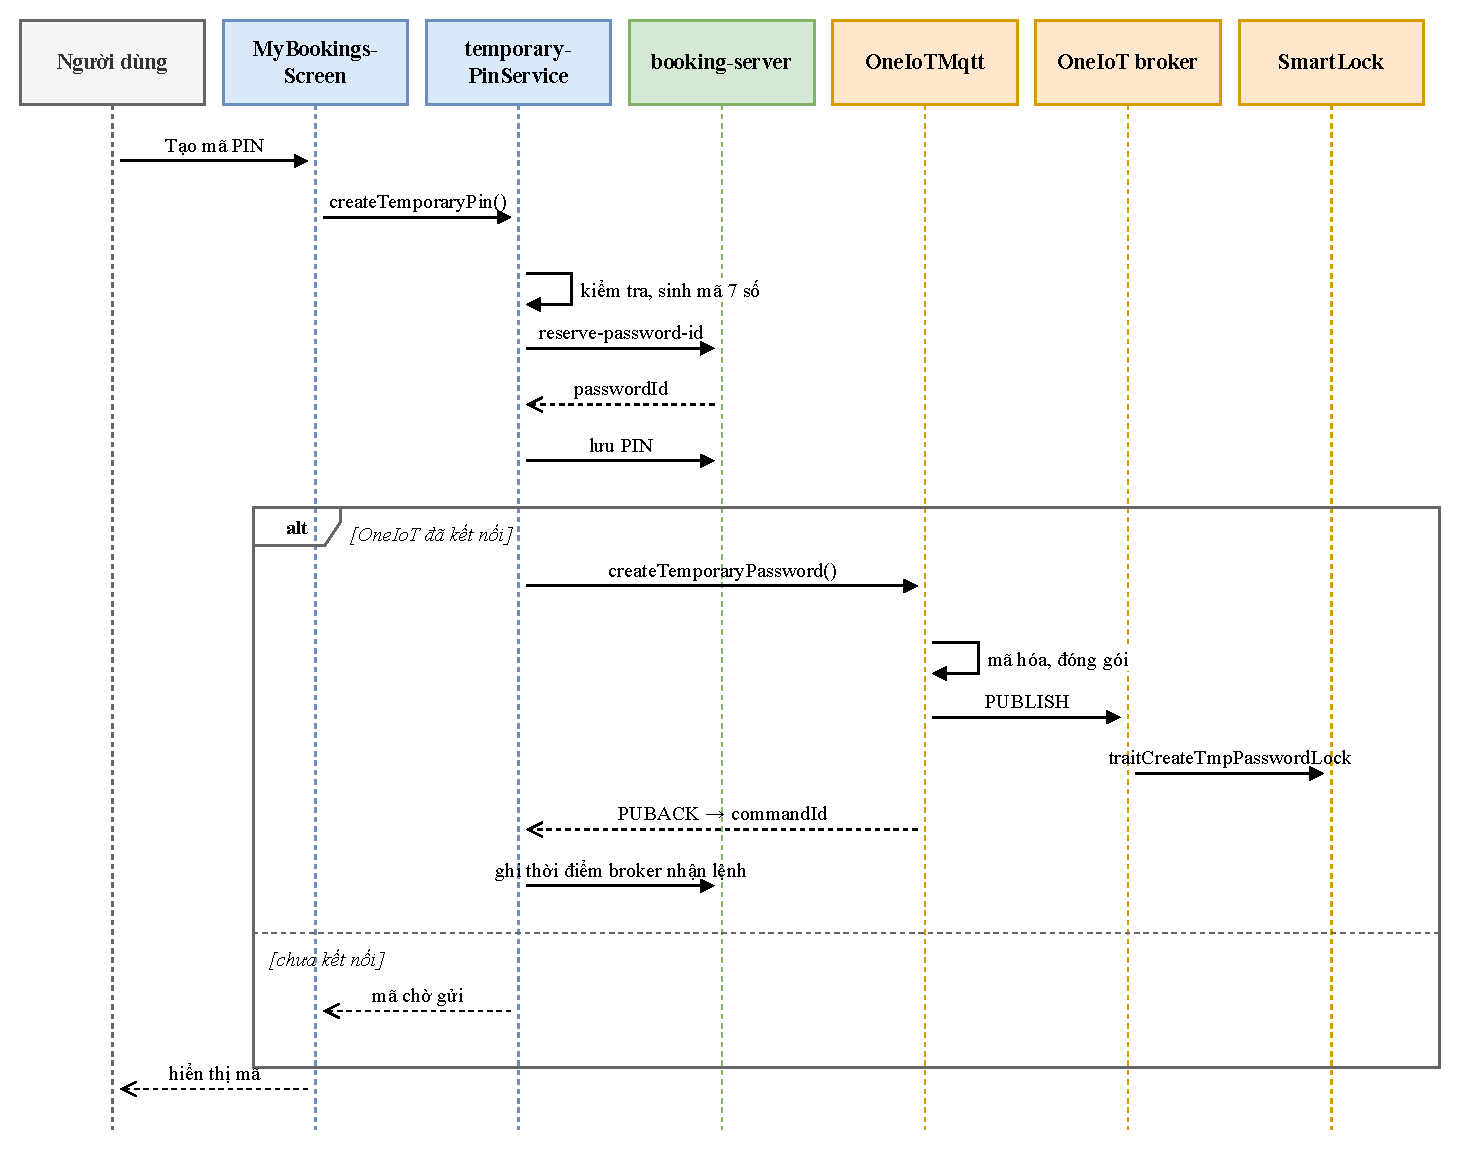
\includegraphics[width=\textwidth,height=.76\textheight,keepaspectratio]{Hinhve/design/16a_sequence_tao_pin_tam.pdf}
\caption{Tạo, lưu và gửi PIN; xác nhận publish của broker tách với thực thi trên khóa}\label{fig:sequence-pin}
\end{figure}

Native \code{OneIoTMqttPackage.kt} chuyển thời hạn sang định dạng bản tin, mã hóa phần mật khẩu và gửi trait \code{traitCreateTmpPasswordLock}. Sau publish được broker xác nhận, app lưu \code{lockDeliveredAt} và request ID. Giao diện cập nhật trạng thái gửi theo kết quả publish; các bản tin sự kiện khóa được xử lý qua luồng nhận MQTT.

\paragraph{Kết quả và hạn chế kỹ thuật.} Các kiểm thử access control và native bridge xác nhận đúng dữ liệu, quyền, thời hạn và cơ chế gửi lại. Ứng dụng và SmartLock thực hiện luồng cấp, sử dụng PIN thực tế. Trạng thái revokedAt quản lý PIN trong booking. Hướng gia cố gồm quản lý ID hữu hạn, bảo vệ dữ liệu, nguồn sinh mã và phản hồi thiết bị.

\FloatBarrier
\subsection{Cùng giao diện nghiệp vụ, hai chế độ dữ liệu}
\label{sec:two-data-solution}
\paragraph{Bài toán.} Hệ thống hỗ trợ vận hành độc lập trên một thiết bị và sử dụng dữ liệu dùng chung qua REST. Hai chế độ dùng cùng giao diện nghiệp vụ để giảm lặp xử lý; nguồn dữ liệu được chọn rõ ràng trong cấu hình bản build.

\paragraph{Giải pháp triển khai.} Repository giữ các hàm nghiệp vụ mà UI gọi; \code{isRemoteApiEnabled} chọn nhánh REST hoặc đọc/ghi JSON local. Client tập trung thêm token và chuyển lỗi mạng/HTTP thành Error cho màn hình. Kiểu TypeScript và cấu trúc request/response Java xác định hợp đồng trao đổi; kiểm thử API kiểm tra phương thức, dữ liệu, phiên và các nhánh lỗi.
{\tabletext\renewcommand{\arraystretch}{1.04}\begin{longtable}{>{\raggedright\arraybackslash}p{\dimexpr0.22\textwidth-2\tabcolsep\relax}>{\raggedright\arraybackslash}p{\dimexpr0.37\textwidth-2\tabcolsep\relax}>{\raggedright\arraybackslash}p{\dimexpr0.41\textwidth-2\tabcolsep\relax}}
\caption{Đối chiếu thao tác local và REST}\label{tab:local-remote}\\
\toprule \textbf{Thao tác} & \textbf{Local} & \textbf{REST}\\\midrule
\endfirsthead
\multicolumn{3}{l}{\small Đối chiếu thao tác local và REST (tiếp)}\\
\toprule \textbf{Thao tác} & \textbf{Local} & \textbf{REST}\\\midrule
\endhead
\bottomrule\endlastfoot
Xác thực & Đọc tài khoản của kho thiết bị, tạo session UI. & Login tạo token/actor tại server; request sau mang Bearer.\\\addlinespace[1.5pt]
Tạo/duyệt booking & Repository kiểm quy tắc trên các tập dữ liệu local và ghi JSON. & API/service kiểm actor và dữ liệu trong giao dịch; server là nơi quyết định trạng thái được lưu.\\\addlinespace[1.5pt]
Phòng/cấu hình/bảo trì & Mỗi máy giữ danh mục và cấu hình riêng. & Các client gọi cùng server sử dụng chung danh mục, cấu hình và dữ liệu phòng.\\\addlinespace[1.5pt]
Quyền và PIN & Quyền và PIN gắn tài khoản/phòng/booking trong kho local. & Quyền và PIN lưu ở server; việc gửi MQTT vẫn xuất phát từ app/native, không chuyển cho Java.\\\addlinespace[1.5pt]
Thông báo & Lưu theo người nhận trong thiết bị; banner chỉ hiện cho tài khoản đang đăng nhập. & Server lưu theo user; client tải thông báo qua REST bằng phiên đăng nhập.\\\addlinespace[1.5pt]
Lỗi kết nối & Không cần booking server; OneIoT vẫn là kết nối riêng nếu dùng khóa. & Trả lỗi/timeout theo client; không tự fallback hoặc tải backlog local.\\\addlinespace[1.5pt]
\end{longtable}}

\paragraph{Kết quả và hạn chế kỹ thuật.} Một nhóm màn hình phục vụ cả hai chế độ; thay đổi cấu hình chọn nguồn dữ liệu mà không chuyển dữ liệu giữa hai kho. Nếu bổ sung offline sync sau này, cần thiết kế định danh, hàng đợi, phiên bản dữ liệu, quy tắc hòa giải và kiểm thử độc lập. Kiểm thử hợp đồng REST duy trì cấu trúc trao đổi giữa app và server; khi mở rộng cần quản lý kết nối, tính sẵn sàng của dịch vụ và dữ liệu dùng chung.


\FloatBarrier
% Ngắt mục lục ở đầu chương 4 để hai trang cân đối.
\addtocontents{toc}{\protect\newpage}
\chapter{TRIỂN KHAI ỨNG DỤNG}\label{chap:implementation}
\section{Môi trường và cấu trúc mã nguồn}
Ứng dụng dùng Community CLI, không dùng Expo. Các thành phần gồm React Native 0.86.2, React 19.2.3, Async Storage 3.1.1, TypeScript 5.9.3 và Jest 29. package.json yêu cầu Node từ 22.11.0. Android cấu hình SDK 36, Kotlin 2.1.20 và native module riêng; backend dùng Java 17/Maven/Spring Boot 3.4.4.

\subsection{Cấu hình công cụ và điều kiện tái lập}
Bảng~\ref{tab:build-config} trình bày công cụ và cấu hình để cài đặt, build và tái lập ứng dụng. Hệ điều hành của thiết bị chạy thử được nêu tại mục 5.1.
{\tabletext\renewcommand{\arraystretch}{1.04}\begin{longtable}{>{\raggedright\arraybackslash}p{\dimexpr0.19\textwidth-2\tabcolsep\relax}>{\raggedright\arraybackslash}p{\dimexpr0.29\textwidth-2\tabcolsep\relax}>{\raggedright\arraybackslash}p{\dimexpr0.52\textwidth-2\tabcolsep\relax}}
\caption{Công cụ và cấu hình biên dịch}\label{tab:build-config}\\
\toprule \textbf{Hạng mục} & \textbf{Cấu hình biên dịch} & \textbf{Tệp đối chiếu}\\\midrule
\endfirsthead
\multicolumn{3}{l}{\small Công cụ và cấu hình biên dịch (tiếp)}\\
\toprule \textbf{Hạng mục} & \textbf{Cấu hình biên dịch} & \textbf{Tệp đối chiếu}\\\midrule
\endhead
\bottomrule\endlastfoot
Node/npm & Node từ 22.11.0; npm cài theo lockfile & \code{code/booking_classroom/package.json}; \code{package-lock.json}.\\\addlinespace[1.5pt]
Android & Compile/target SDK 36; min SDK 24; Build-Tools 36.0.0 & \code{android/build.gradle}; \code{android/app/build.gradle}, tính từ thư mục app.\\\addlinespace[1.5pt]
Native build & NDK 27.1.12297006; Kotlin 2.1.20; Gradle wrapper 9.3.1 & \code{android/build.gradle}; \code{android/gradle/wrapper/gradle-wrapper.properties}.\\\addlinespace[1.5pt]
Bản Android & Package com.bookingclassroom; versionName 1.0; versionCode 1 & \code{android/app/build.gradle}; version npm 0.0.1 là trường riêng trong package.json.\\\addlinespace[1.5pt]
Backend & Java 17; Spring Boot 3.4.4; H2 file mặc định & \code{code/booking-server/pom.xml}; \code{src/main/resources/application.properties}.\\\addlinespace[1.5pt]
\end{longtable}}

Máy build cần JDK, Android SDK và Platform-Tools/ADB được cấu hình đúng đường dẫn; Windows dùng PowerShell cho script hiện có. Các phiên bản và tên thiết bị trong hồ sơ kiểm thử được trình bày riêng ở Chương~\ref{chap:testing}.

\subsection{Cấu trúc mã nguồn và trách nhiệm triển khai}

Các đường dẫn trong chương tính từ repository \code{final_project/}. Mã nguồn ứng dụng ở \code{code/booking_classroom/}, backend ở \code{code/booking-server/}. Cấu trúc thực tế được tóm tắt như sau:
{\small\renewcommand{\arraystretch}{1.1}
\begin{longtable}{>{\raggedright\arraybackslash}p{\dimexpr.49\textwidth-2\tabcolsep\relax}>{\raggedright\arraybackslash}p{\dimexpr.51\textwidth-2\tabcolsep\relax}}
\caption{Cấu trúc thư mục và trách nhiệm}\label{tab:source-tree}\\
\toprule\textbf{Vị trí trong repository} & \textbf{Vai trò}\\\midrule
\endfirsthead
\multicolumn{2}{l}{Cấu trúc thư mục và trách nhiệm (tiếp)}\\
\toprule\textbf{Vị trí trong repository} & \textbf{Vai trò}\\\midrule
\endhead
\bottomrule\endlastfoot
\code{code/booking_classroom/App.tsx} & Điểm ghép giao diện và phiên của app.\\\addlinespace[1.5pt]
\code{code/booking_classroom/src/app/} & Ghép màn hình theo vai trò.\\\addlinespace[1.5pt]
\code{code/booking_classroom/src/core/} & API, storage, time, config và types dùng chung.\\\addlinespace[1.5pt]
\code{code/booking_classroom/src/modules/} & 11 module nghiệp vụ.\\\addlinespace[1.5pt]
\code{code/booking_classroom/src/shared/} & Thành phần UI dùng chung.\\\addlinespace[1.5pt]
\code{code/booking_classroom/android/app/src/} & Native Android.\\\addlinespace[1.5pt]
\code{code/booking_classroom/__tests__/}; \code{code/booking_classroom/quality-tests/} & Test ứng dụng và bộ kiểm thử chất lượng riêng.\\\addlinespace[1.5pt]
\code{code/booking-server/src/main/java/} & Gói com/bookingclassroom/server/: service, entity, session; thư mục api/ có sáu controller.\\\addlinespace[1.5pt]
\code{code/booking-server/src/main/resources/} & Cấu hình backend.\\\addlinespace[1.5pt]
\code{code/booking-server/src/test/} & Kiểm thử tích hợp H2.\\
\end{longtable}}

Màn hình tiếp nhận thao tác và hiển thị dữ liệu; dịch vụ kiểm tra nghiệp vụ trước khi đọc/ghi qua repository. Model xác định kiểu dữ liệu trao đổi. Nghiệp vụ đặt phòng phối hợp với phòng, cấu hình, bảo trì, cấp quyền, tự duyệt và thông báo; phép kiểm giao thời gian được dùng chung để giữ nhất quán.

\section{Ánh xạ yêu cầu chức năng tới mã nguồn}
Trong Bảng~\ref{tab:fr-code}, tiền tố file app là \code{code/booking_classroom/}; phần tên hàm mô tả điểm triển khai cụ thể.
{\tabletext\renewcommand{\arraystretch}{1.04}\begin{longtable}{>{\raggedright\arraybackslash}p{\dimexpr0.08\textwidth-2\tabcolsep\relax}>{\raggedright\arraybackslash}p{\dimexpr0.49\textwidth-2\tabcolsep\relax}>{\raggedright\arraybackslash}p{\dimexpr0.43\textwidth-2\tabcolsep\relax}}
\caption{Ánh xạ chức năng, vị trí và bằng chứng}\label{tab:fr-code}\\
\toprule \textbf{FR} & \textbf{Màn hình / vị trí xử lý} & \textbf{Hành vi và minh chứng}\\\midrule
\endfirsthead
\multicolumn{3}{l}{\small Ánh xạ chức năng, vị trí và bằng chứng (tiếp)}\\
\toprule \textbf{FR} & \textbf{Màn hình / vị trí xử lý} & \textbf{Hành vi và minh chứng}\\\midrule
\endhead
\bottomrule\endlastfoot
FR01 & \code{src/modules/auth/screens/LoginScreen.tsx}; \code{src/modules/auth/services/accountRepository.ts}. & Đăng nhập cập nhật phiên và mở màn hình đúng vai trò; đăng ký, đổi/khôi phục mật khẩu kiểm dữ liệu và phản hồi lỗi. TC01, TC17; D01--D03.\\\addlinespace[1.5pt]
FR02 & \code{src/modules/room_management/screens/RoomSearchScreen.tsx}; \code{src/modules/room_management/services/roomRepository.ts}. & Bộ lọc kết hợp danh mục, booking và bảo trì để hiển thị phòng khả dụng. Hình~\ref{fig:ui-booking}; TC02, TC12.\\\addlinespace[1.5pt]
FR03 & \code{src/modules/booking/services/bookingRepository.ts}; \code{src/modules/booking/screens/MyBookingsScreen.tsx}. & Kiểm từng lượt trước khi lưu chuỗi; hủy/sửa theo quyền, trạng thái và hạn chót. TC11--TC12, TC21.\\\addlinespace[1.5pt]
FR04 & \code{src/modules/booking/screens/AdminBookingScreen.tsx}; \code{src/modules/auto_approval/model/approvalPolicy.ts}. & Duyệt tay theo quyền admin; tự duyệt sau kiểm tra hợp lệ khi phòng thường và cấu hình cho phép. TC07, TC20, TC24.\\\addlinespace[1.5pt]
FR05 & \code{src/modules/access_control/services/temporaryPinService.ts}; \code{src/modules/booking/services/bookingRepository.ts}. & Kiểm chủ lượt/quyền phòng, lưu PIN và gửi qua OneIoT; trao đổi lịch nhận chìa và ủy quyền. TC03, TC10, TC13--TC15, TC19.\\\addlinespace[1.5pt]
FR06 & \code{src/modules/smart_lock/services/smartLockAccessEventService.ts}; \code{src/modules/booking/services/bookingRepository.ts}. & Tiếp nhận sự kiện khóa, ghi nhận có mặt/ra và chặn no-show khi đã có check-in. TC10, TC22.\\\addlinespace[1.5pt]
FR07 & \code{src/modules/schedule_maintenance/services/maintenanceRepository.ts}; \code{src/modules/booking/services/bookingRepository.ts}. & Tách ghi chú, yêu cầu bảo trì và lịch chặn phòng; admin xử lý theo trạng thái. TC02, TC23.\\\addlinespace[1.5pt]
FR08 & \code{src/modules/account_management/}; \code{src/modules/configuration/}; \code{src/modules/profile/}; \code{src/modules/notifications/}. & Quản trị theo quyền; lưu hồ sơ/cấu hình và thông báo theo người nhận. TC06, TC08--TC09, TC16, TC18.\\\addlinespace[1.5pt]
\end{longtable}}

Màn tìm và đặt nằm trong room\_management nhưng gọi nghiệp vụ booking; quản lý tài khoản có UI riêng nhưng dùng accountRepository của auth. Phân quyền online được kiểm thêm ở filter/service Java, không dựa riêng vào việc UI ẩn nút.

\Needspace{13\baselineskip}
\section{Ma trận kỹ thuật React Native}
{\tabletext\renewcommand{\arraystretch}{1.04}\begin{longtable}{>{\raggedright\arraybackslash}p{\dimexpr0.19\textwidth-2\tabcolsep\relax}>{\raggedright\arraybackslash}p{\dimexpr0.55\textwidth-2\tabcolsep\relax}>{\raggedright\arraybackslash}p{\dimexpr0.26\textwidth-2\tabcolsep\relax}}
\caption{Kỹ thuật, cách áp dụng, lý do và kiểm chứng}\label{tab:rn}\\
\toprule \textbf{Kỹ thuật} & \textbf{Vị trí và cách áp dụng / lý do} & \textbf{Bằng chứng}\\\midrule
\endfirsthead
\multicolumn{3}{l}{\small Kỹ thuật, cách áp dụng, lý do và kiểm chứng (tiếp)}\\
\toprule \textbf{Kỹ thuật} & \textbf{Vị trí và cách áp dụng / lý do} & \textbf{Bằng chứng}\\\midrule
\endhead
\bottomrule\endlastfoot
Component, JSX, Props & \code{App.tsx}: App truyền session/onLogout cho RoleDashboardScreen và onLogin cho LoginScreen. Props/callback tập trung phiên ở gốc, tránh sao chép trạng thái xác thực. & Đoạn A; TC01, D02.\\\addlinespace[1.5pt]
State & \code{src/modules/auth/screens/LoginScreen.tsx}: LoginScreen dùng useState cho input, error và submitting. Trạng thái cục bộ đáp ứng biểu mẫu; useReducer không áp dụng. & TC01, TC17; D01--D03.\\\addlinespace[1.5pt]
Effect và cleanup & \code{App.tsx}: App.useEffect đăng ký AppState/sự kiện khóa rồi tháo listener và ngắt MQTT; \code{src/modules/auth/screens/LoginScreen.tsx}: effect xử lý BackHandler. Cleanup tránh lặp bộ lắng nghe khi chuyển màn. & App, dòng 24--38; kiểm thử bridge và callback.\\\addlinespace[1.5pt]
Custom Hook / Context / Store & Không áp dụng ở tầng nghiệp vụ: quy mô hiện tại dùng state cục bộ, props và service; chưa cần store dùng chung. & Cấu trúc phụ thuộc ở mục 4.1; đoạn A.\\\addlinespace[1.5pt]
Điều hướng & \code{src/app/screens/RoleDashboardScreen.tsx}: RoleDashboardScreen dùng activeScreen, closeChildScreen và onBack; giữ điều hướng tập trung cho số màn hiện tại. & Hình~\ref{fig:flow-user}--\ref{fig:flow-admin}; D02.\\\addlinespace[1.5pt]
Async, API, Promise & \code{src/core/api/client.ts}: apiRequest dùng fetch, AbortController và finally; tập trung token, giới hạn chờ và chuyển lỗi cho UI. & Đoạn B; TC04--TC05.\\\addlinespace[1.5pt]
Form và validation & \code{src/modules/auth/screens/LoginScreen.tsx}: submit kiểm dữ liệu, đặt submitting, gọi authenticate và khôi phục trạng thái trong finally; kiểm lại ở service để bảo vệ nghiệp vụ. & TC01, TC17; D01, D03.\\\addlinespace[1.5pt]
Danh sách & \code{src/modules/room_management/}\par\code{screens/RoomSearchScreen.tsx}: RoomSearchScreen dùng ScrollView/map và key theo định danh, phù hợp danh mục hiện tại. FlatList/phân trang không áp dụng. & Hình~\ref{fig:ui-booking}; kiểm thử bộ lọc.\\\addlinespace[1.5pt]
Lưu trữ và quyền & \code{src/core/storage/jsonStorage.ts}: readJson/writeJson bọc Async Storage; \code{src/modules/notifications/services/priorityBanner.ts}: requestPriorityNotificationPermission xử lý API 33+. Tách lưu trữ khỏi UI và xin quyền theo nền tảng. & TC08--TC09; D05--D06.\\\addlinespace[1.5pt]
Tối ưu / nền tảng & \code{src/app/screens/RoleDashboardScreen.tsx}: refreshUnreadCount dùng useCallback để ổn định dependency của effect; \code{src/modules/notifications/services/priorityBanner.ts} kiểm Platform.OS trước khi gọi native. & Kiểm thử quyền API 31/33 và bản chạy Android.\\\addlinespace[1.5pt]
\end{longtable}}

\section{Phân tích hai đoạn mã cốt lõi}
\par\noindent\begin{minipage}{\linewidth}
\setlength{\parindent}{1cm}
\subsection{Đoạn A: giao diện, phiên và callback}
\textbf{Tệp:} \coderef{code/booking_classroom/App.tsx}, dòng 40--62. Liên quan FR01/FR08 và G03. Đầu vào là session do useState ở dòng 18 giữ; đầu ra là cây component theo trạng thái xác thực.
\VerbatimInput[fontsize=\small,numbers=left,numbersep=5pt,firstnumber=40,firstline=40,lastline=62,breaklines=true,frame=single]{../../../../code/booking_classroom/App.tsx}

\end{minipage}\par\smallskip
\textbf{Phân tích.} Dòng 47 rẽ nhánh bằng session; 48--55 truyền dữ liệu và callback cho màn theo vai trò. Dòng 50--53 gom logout: ngắt OneIoT, xóa token, đặt session null. Dòng 57 truyền setSession làm onLogin; khi LoginScreen hoàn tất authenticate, callback làm App render lại. Props/callback duy trì một chủ sở hữu phiên, không sao chép mật khẩu vào state toàn app.

Trạng thái lỗi/loading thuộc LoginScreen: submit kiểm ô trống, đặt submitting, xử lý null/error rồi khôi phục trạng thái trong finally. Effect tại App dòng 24--38 đăng ký listener và dọn dẹp khi unmount/xuống nền \cite{react}. Người dùng đăng nhập lại sau khi mở ứng dụng; MQTT hoạt động theo phiên kết nối. App.test/authScreens kiểm giao diện và điều hướng; thử nghiệm trên thiết bị xác nhận quá trình sử dụng cùng SmartLock.

\par\noindent\begin{minipage}{\linewidth}
\setlength{\parindent}{1cm}
\subsection{Đoạn B: xử lý HTTP bất đồng bộ và ngoại lệ}
\textbf{Tệp:} \coderef{code/booking_classroom/src/core/api/client.ts}, dòng 35--61. Liên quan FR01--FR08/NFR02. Đầu vào là path, method, body và token của phiên; đầu ra là response JSON hoặc Error cho màn hình.
\VerbatimInput[fontsize=\small,numbers=left,numbersep=5pt,firstnumber=35,firstline=35,lastline=61,breaklines=true,frame=single]{../../../../code/booking_classroom/src/core/api/client.ts}

\end{minipage}\par\smallskip
\textbf{Phân tích.} Dòng 36--37 tạo controller và timer giới hạn chờ. Dòng 39--42 chuẩn hóa/kiểm URL; 43--52 đóng gói request, thêm Bearer nếu có, serialize body và gắn signal. Dòng 53--58 chuyển lỗi mạng/abort thành thông điệp nghiệp vụ; finally 59--61 xóa timer dù thành công hay lỗi.

Phần sau trích đoạn xử lý 204, parse JSON, thông báo lỗi HTTP và xóa token khi 401. Client không tự retry để tránh lặp thao tác ghi, không tự fallback local vì hai kho không hòa giải. Kiểm thử HTTP mô phỏng fetch và timer để xác nhận header, body, lỗi JSON, lỗi 401, mất mạng và ngắt yêu cầu sau 12 giây (TC04--TC05). Đây là kiểm tra cơ chế giới hạn chờ ở client.

\Needspace{17\baselineskip}
\section{Truy vết luồng đăng nhập và xử lý ngoại lệ}
{\tabletext\renewcommand{\arraystretch}{1.04}\begin{longtable}{>{\raggedright\arraybackslash}p{\dimexpr0.3\textwidth-2\tabcolsep\relax}>{\raggedright\arraybackslash}p{\dimexpr0.44\textwidth-2\tabcolsep\relax}>{\raggedright\arraybackslash}p{\dimexpr0.26\textwidth-2\tabcolsep\relax}}
\caption{Từ thao tác tới render trong luồng đăng nhập}\label{tab:trace}\\
\toprule \textbf{Bước / vị trí} & \textbf{Dữ liệu và trạng thái} & \textbf{Kiểm chứng}\\\midrule
\endfirsthead
\multicolumn{3}{l}{\small Từ thao tác tới render trong luồng đăng nhập (tiếp)}\\
\toprule \textbf{Bước / vị trí} & \textbf{Dữ liệu và trạng thái} & \textbf{Kiểm chứng}\\\midrule
\endhead
\bottomrule\endlastfoot
1. LoginScreen onChange/submit & TextInput cập nhật username/password. Thiếu ô bắt buộc đặt error; không gửi request. & AuthScreens quality và giao diện đăng nhập.\\\addlinespace[1.5pt]
2. submit / authenticate & submitting=true, xóa/ghi error theo kết quả; local đọc auth.accounts hoặc REST gọi login. & Auth unit/component; apiClient mock.\\\addlinespace[1.5pt]
3. accountRepository / apiRequest & REST nhận token/role; lỗi xác thực trả null theo điều kiện. Mạng lỗi/timeout thành Error, 401 xóa token. & Test sai mật khẩu, duplicate và các ca API lỗi.\\\addlinespace[1.5pt]
4. onLogin / App.setSession & Thành công truyền username/role, render RoleDashboard theo role; không truyền mật khẩu. & App.test; biên bản Admin/User.\\\addlinespace[1.5pt]
5. finally / cleanup & submitting=false để mở lại nút. BackHandler/listener bị tháo khi màn tương ứng đóng; logout/ngắt nền đóng MQTT. & Source submit/useEffect; native bridge được mock.\\\addlinespace[1.5pt]
\end{longtable}}

Khi xác thực thất bại hoặc mất kết nối REST, ứng dụng giữ người dùng ở biểu mẫu và hiển thị thông điệp lỗi cụ thể. Dữ liệu local thiếu được repository khởi tạo theo model; dữ liệu remote lỗi định dạng bị API client từ chối. Các màn giữ loading/error bằng state; cập nhật state làm component render lại.

\section{Giao diện và sản phẩm chạy thử}
Chín ảnh giao diện minh họa các bước thao tác và nhóm chức năng của ứng dụng, từ đăng nhập, đặt phòng đến quản lý và cấu hình. Các luồng này được kết hợp kiểm thử tự động và chạy thực tế trên thiết bị.

\subsection{Đăng nhập và phân tách chức năng theo vai trò}
Hình~\ref{fig:ui-roles} gồm đăng nhập và hai dashboard. Kết quả xác thực xác định vai trò và nhóm chức năng hiển thị; tầng dịch vụ tiếp tục kiểm quyền đối với từng thao tác. Đổi tài khoản cập nhật phiên, xóa token REST và ngắt OneIoT khi đăng xuất.

Màn hình đăng nhập sử dụng các trường tài khoản, mật khẩu và thông báo lỗi. Kiểm thử xác thực xác nhận các ô bắt buộc, sai mật khẩu, chuyển biểu mẫu và mở chức năng đúng vai trò (TC01, TC17 và D01--D03).

\begin{figure}[H]\centering
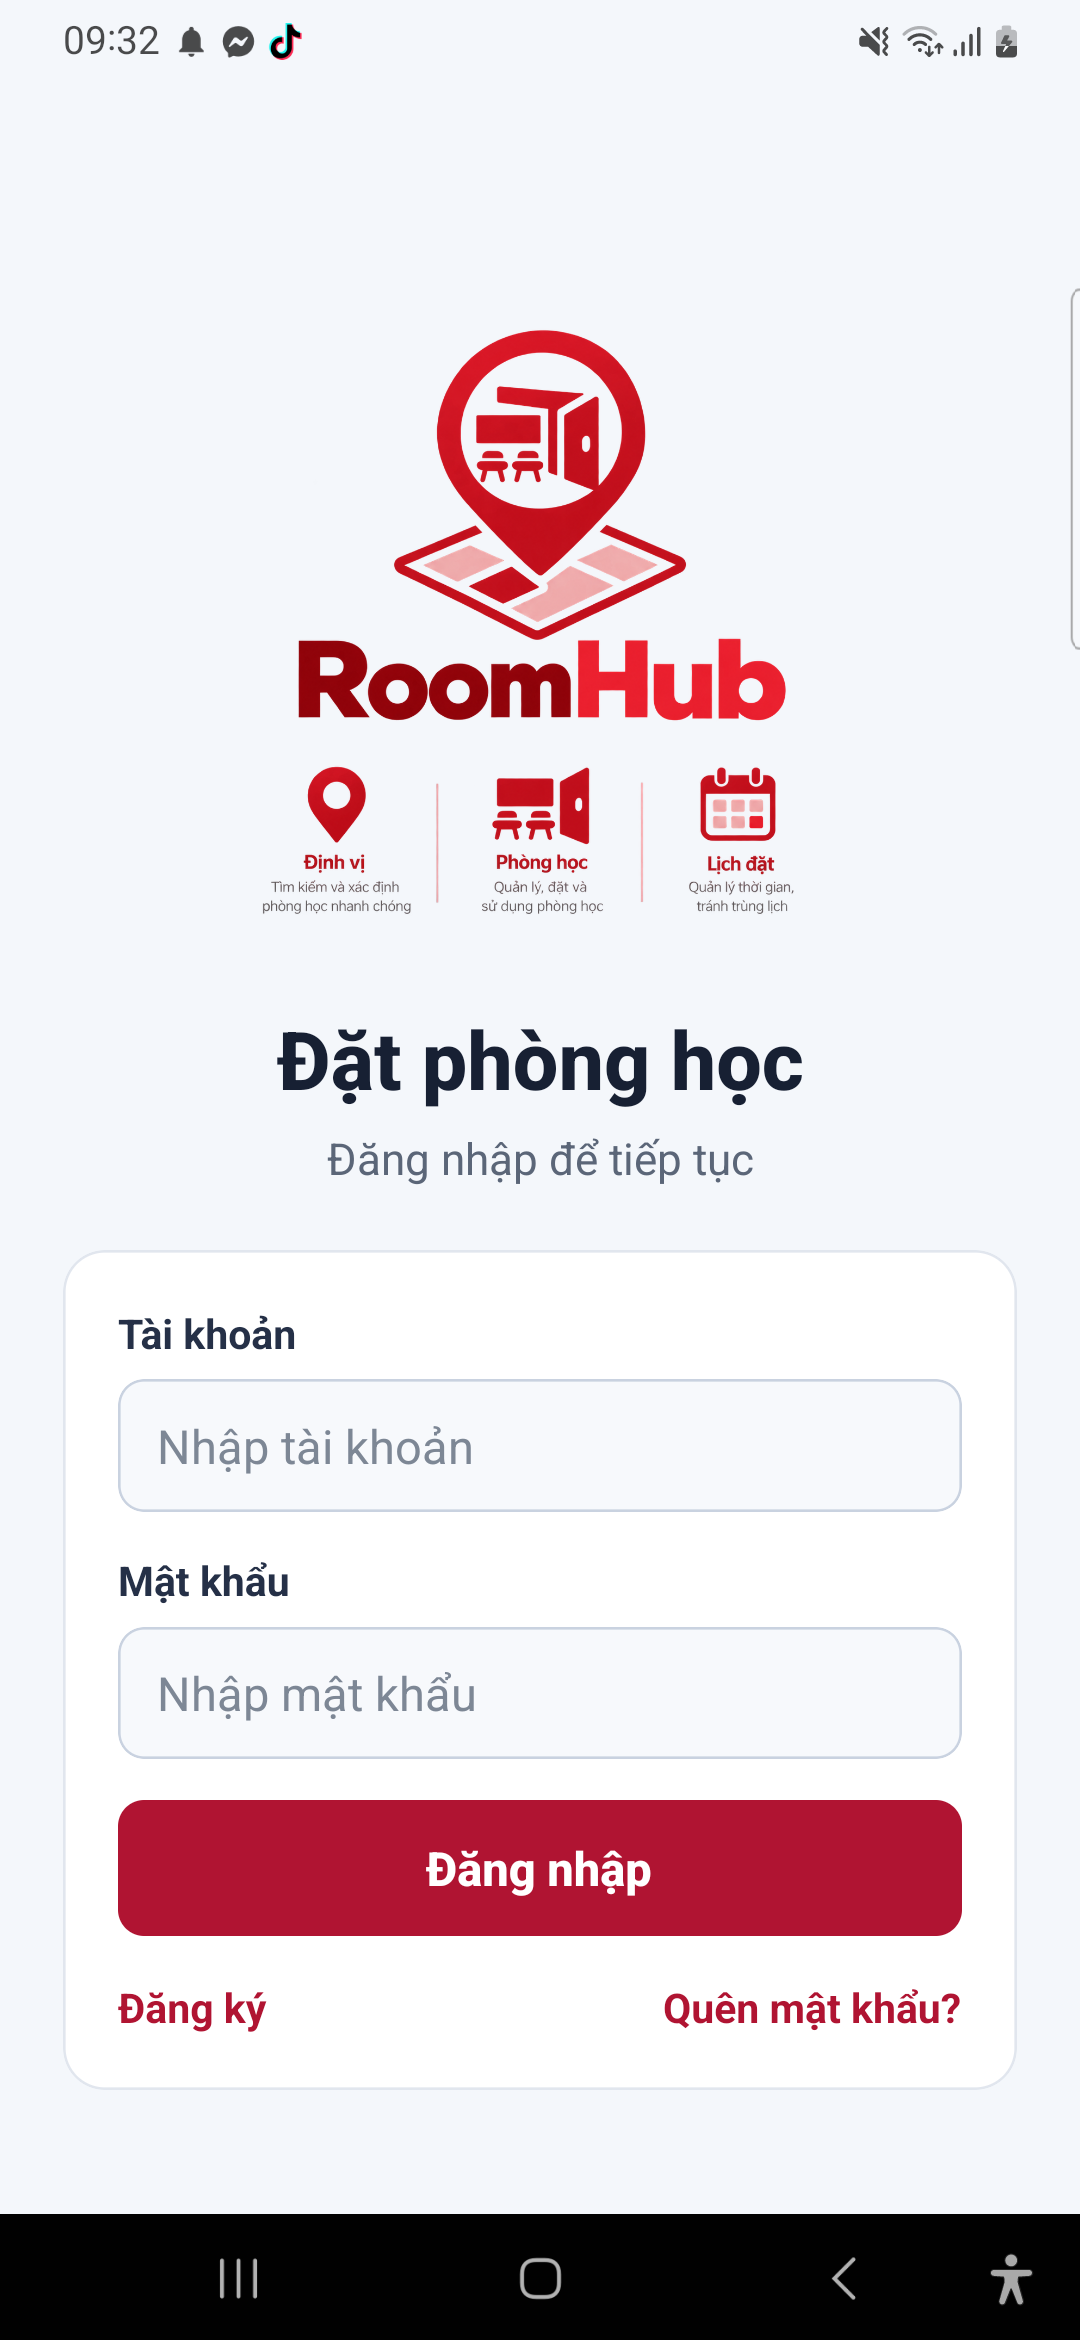
\includegraphics[height=7.8cm]{Hinhve/login_hien_tai.png}\hspace{.6cm}
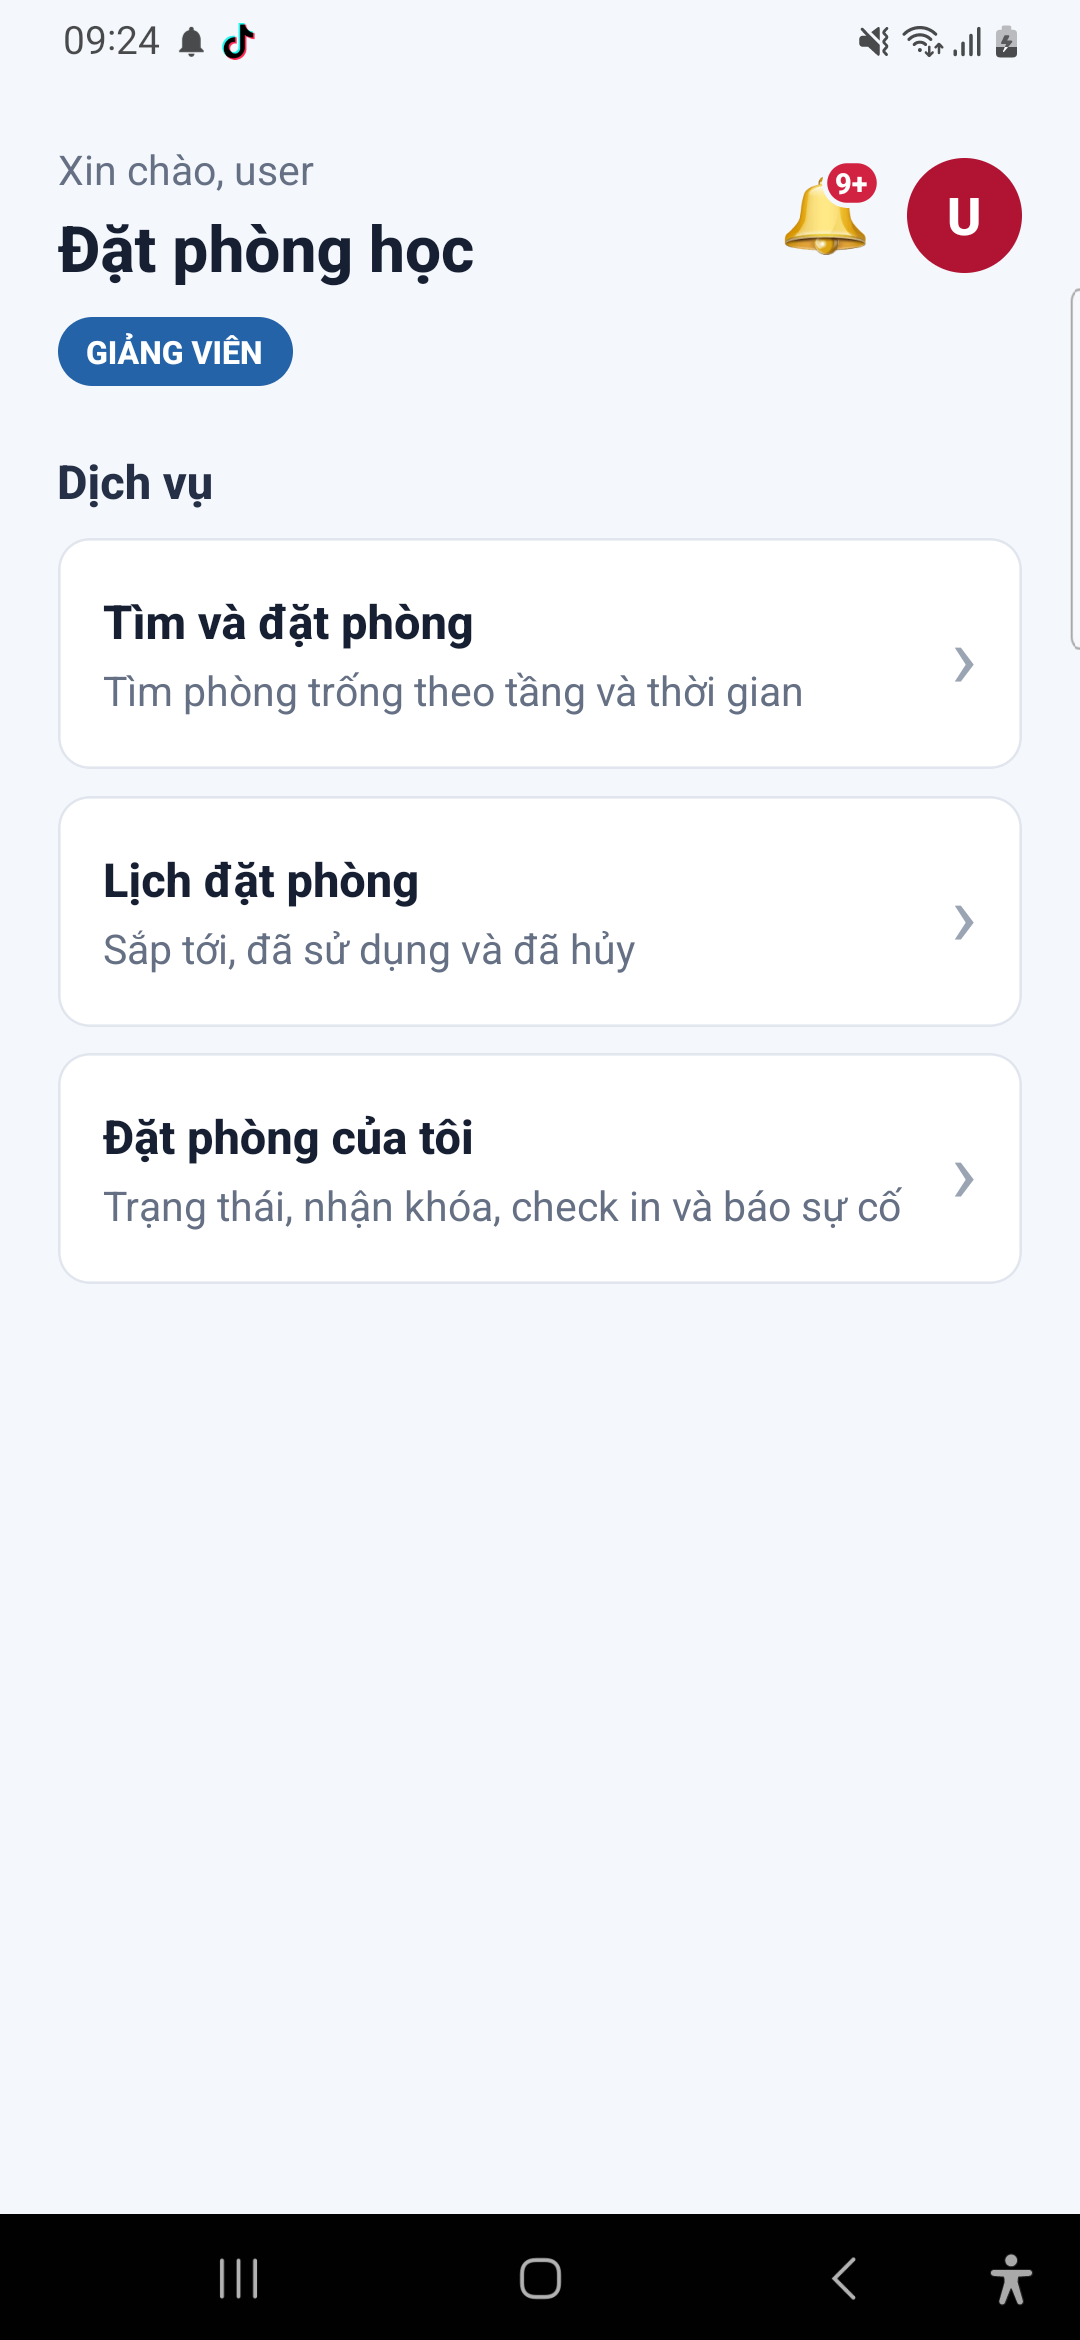
\includegraphics[height=7.8cm]{Hinhve/giao_dien_nguoi_dung_hien_tai.png}\hspace{.6cm}
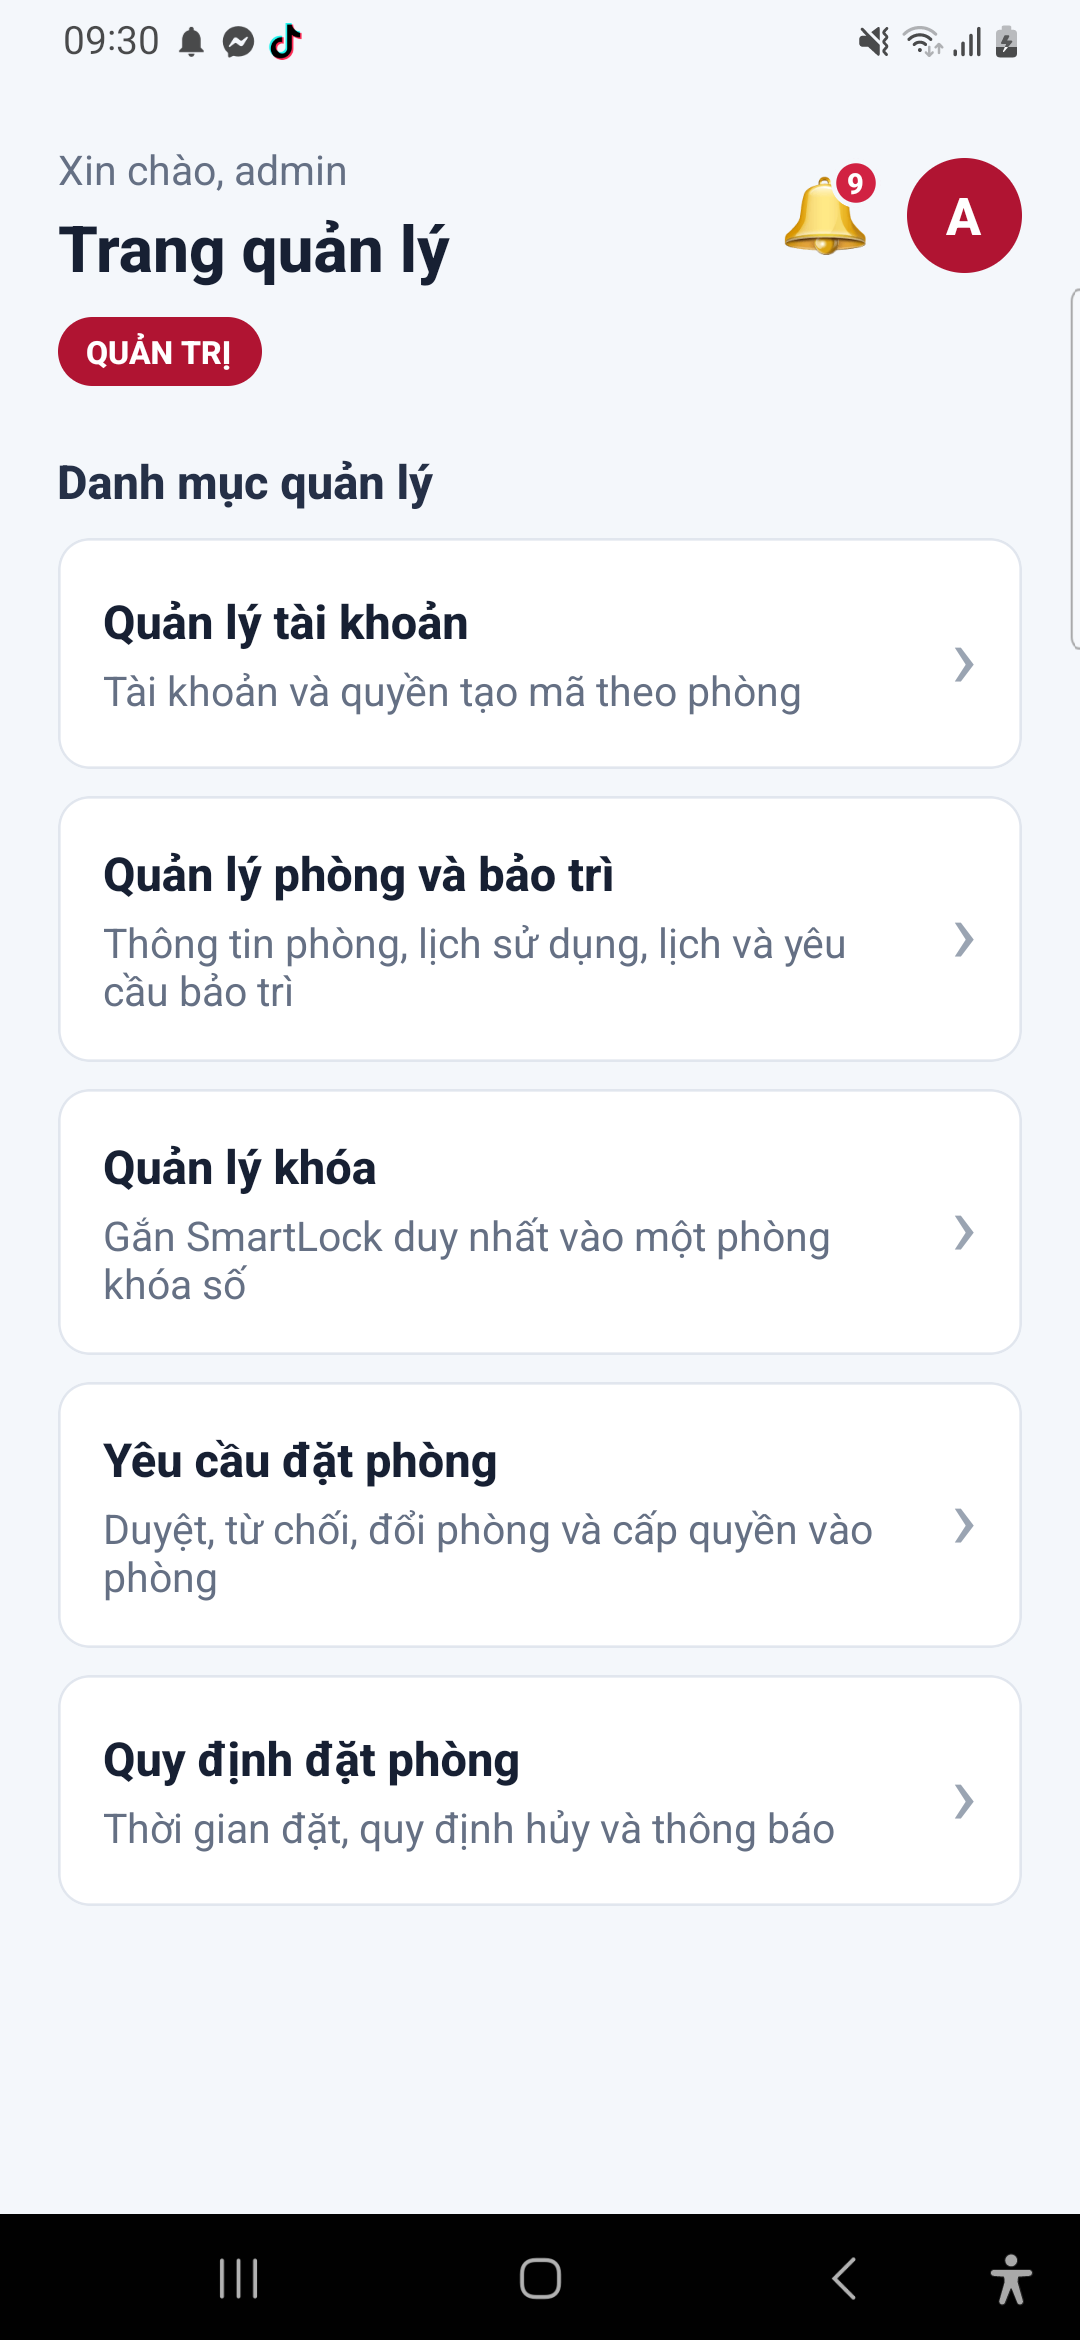
\includegraphics[height=7.8cm]{Hinhve/giao_dien_admin_hien_tai.png}
\caption{Đăng nhập, chức năng User và Admin (trái sang phải)}\label{fig:ui-roles}
\end{figure}
\subsection{Tìm và gửi yêu cầu trên cùng màn hình}
Hình~\ref{fig:ui-booking} giữ hai bước: chọn tầng/ngày/giờ, sức chứa/thiết bị/loại khóa; rồi chọn phòng, nhập mục đích và gửi. Ứng dụng tải danh mục và mức chiếm chỗ để hỗ trợ lựa chọn; khi gửi yêu cầu, tầng nghiệp vụ kiểm lại lịch và các quy tắc trước khi ghi. Tám tầng là dữ liệu demo.

\begin{figure}[H]\centering
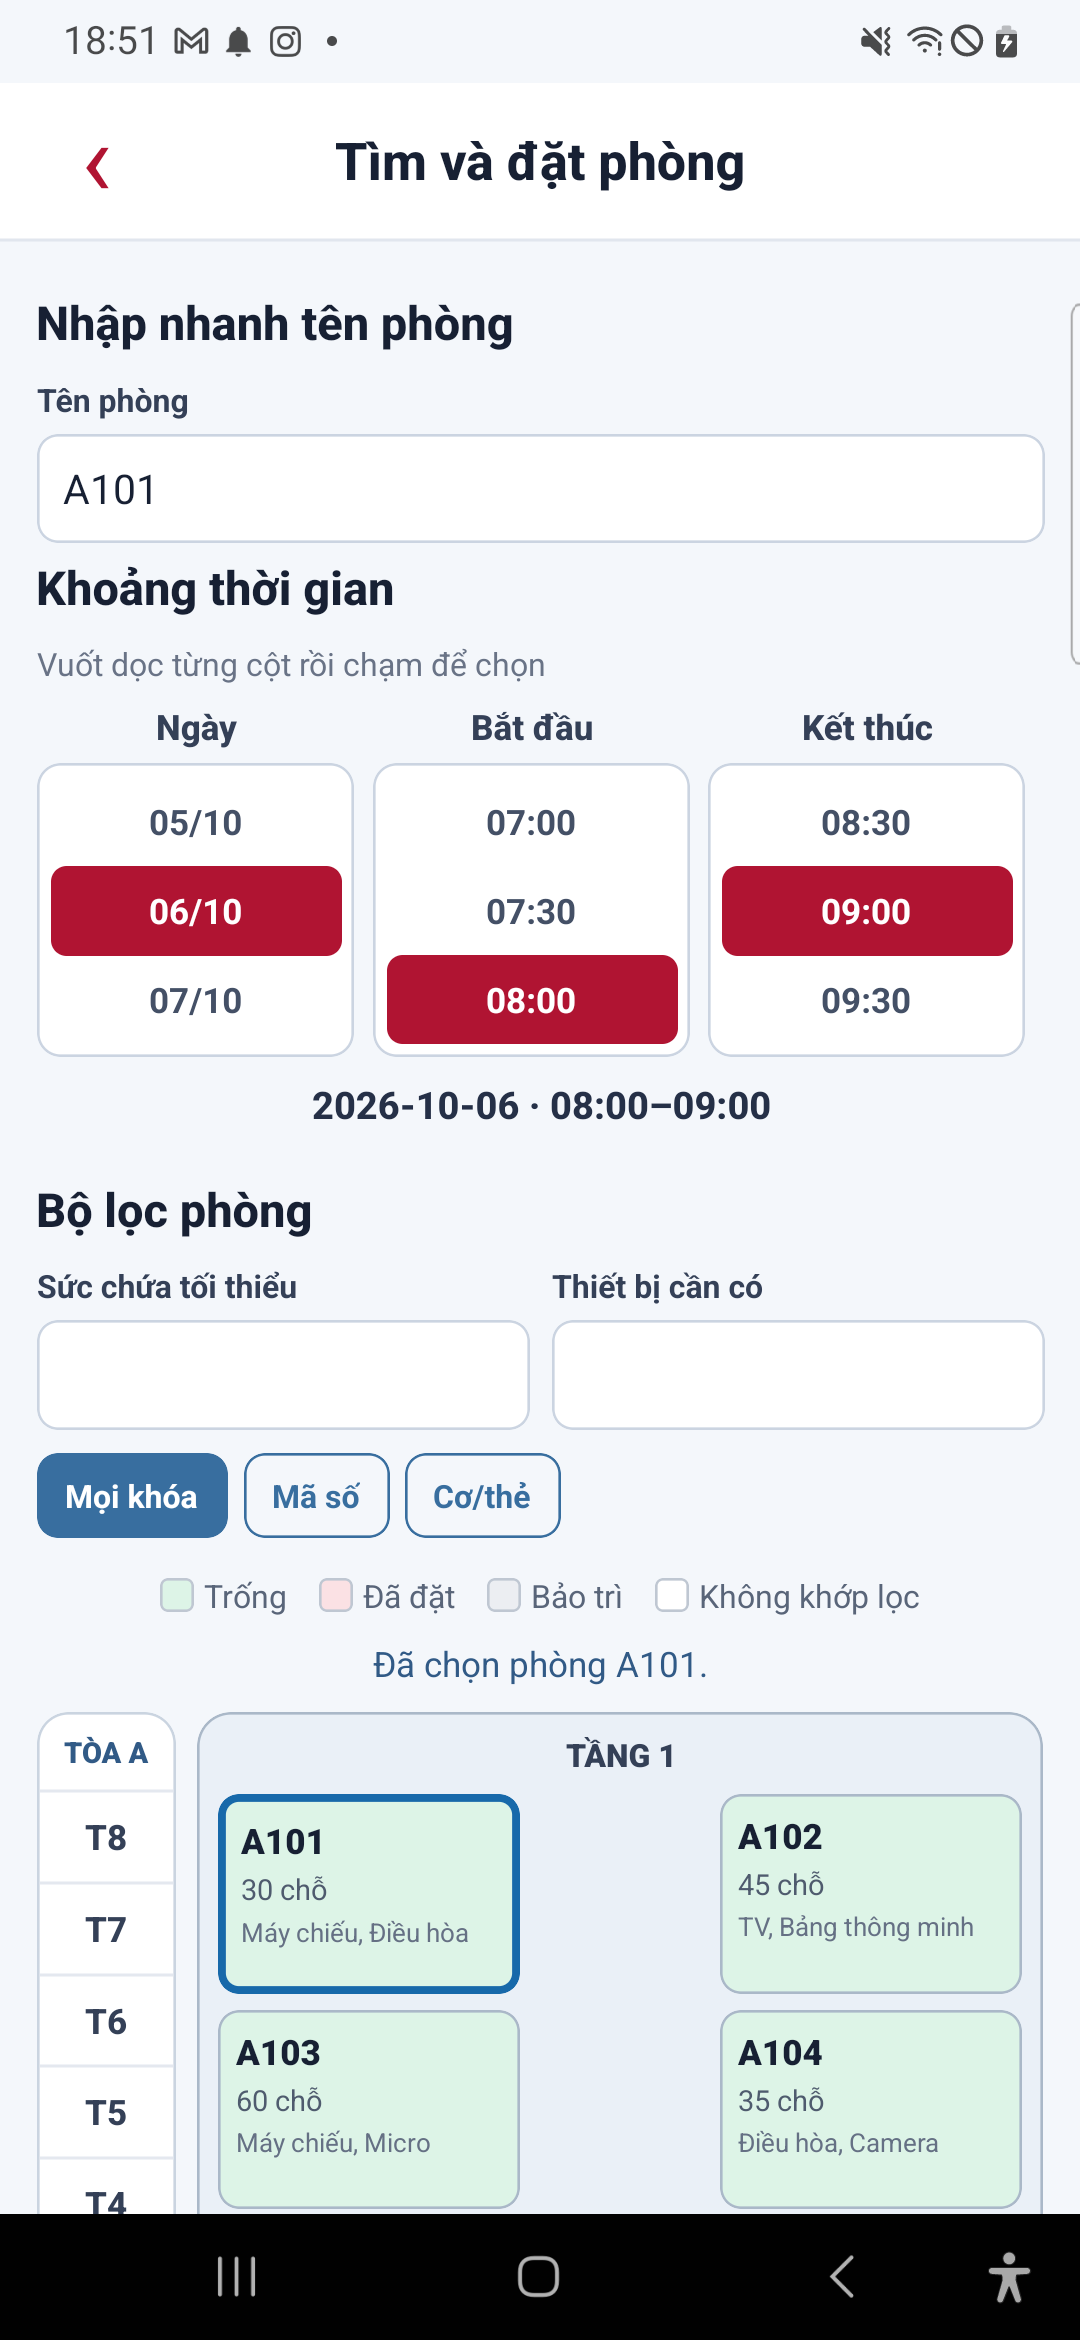
\includegraphics[height=8cm]{Hinhve/tim_va_dat_phong_hien_tai.png}\hspace{1.2cm}
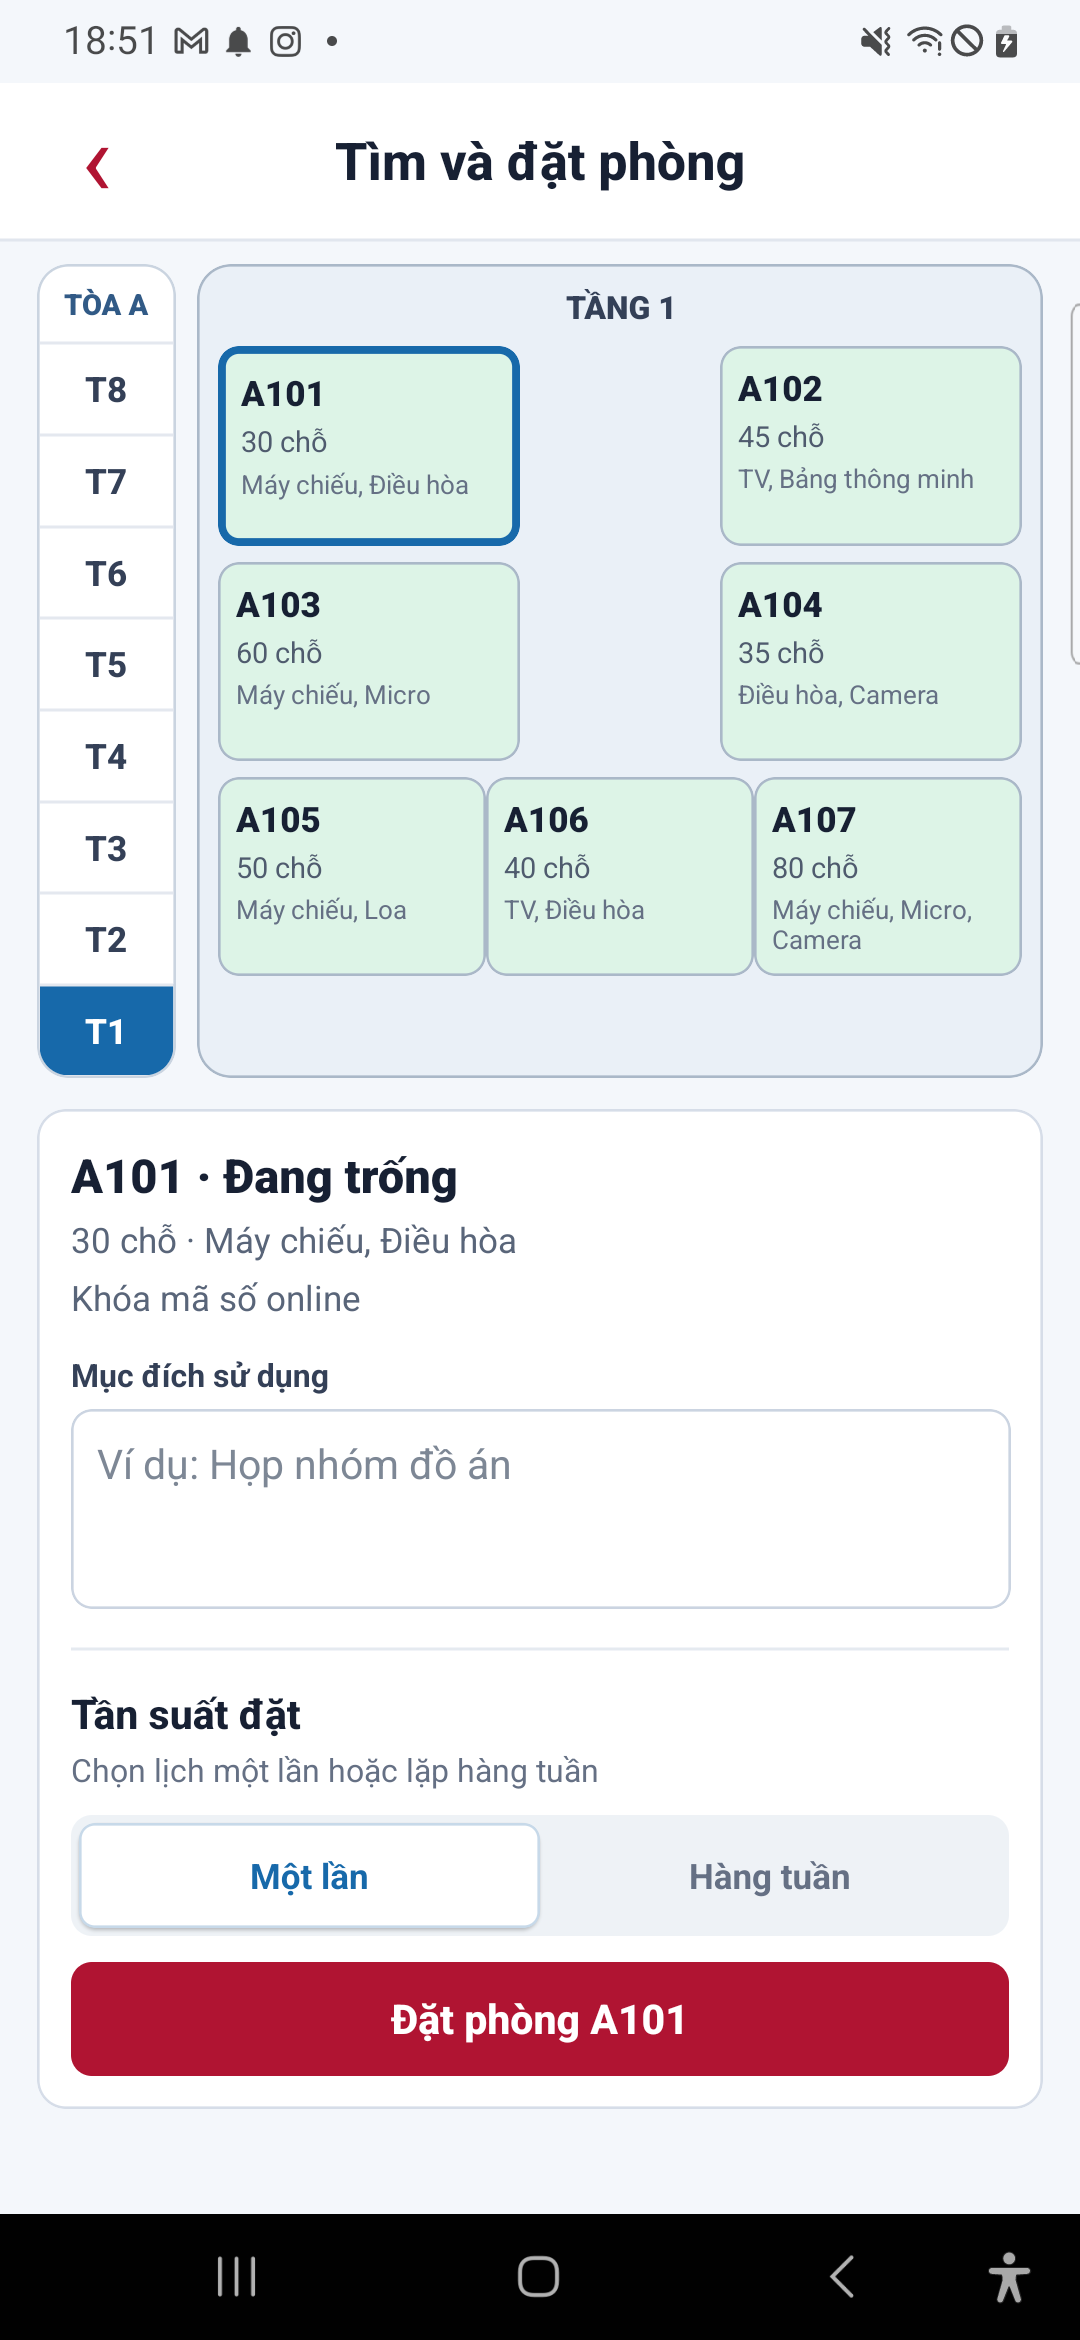
\includegraphics[height=8cm]{Hinhve/chon_phong_va_dat_hien_tai.png}
\caption{Chọn tiêu chí, chọn phòng và gửi yêu cầu (trái sang phải)}\label{fig:ui-booking}
\end{figure}
\subsection{Quản lý phòng và bảo trì theo tầng}
Hình~\ref{fig:ui-room-maintenance} gồm danh sách tầng thu gọn có số phòng/chỉ báo bảo trì và tầng đã mở với thông tin từng phòng. Các tầng có thể mở/thu gọn; trạng thái phòng được tổng hợp từ danh mục, lượt đặt, yêu cầu và lịch bảo trì.

Admin chọn phòng để sửa/xóa, xem hoặc lập/hủy lịch bảo trì. Service chặn xóa phòng còn booking hoạt động; phòng mẫu đã xóa được lưu dấu để không tự tái xuất hiện. Yêu cầu bảo trì phải qua tiếp nhận/lên lịch mới chặn phòng; ghi chú chỉ thông báo admin (UC08, UC13; TC02, TC23).

\begin{figure}[H]\centering
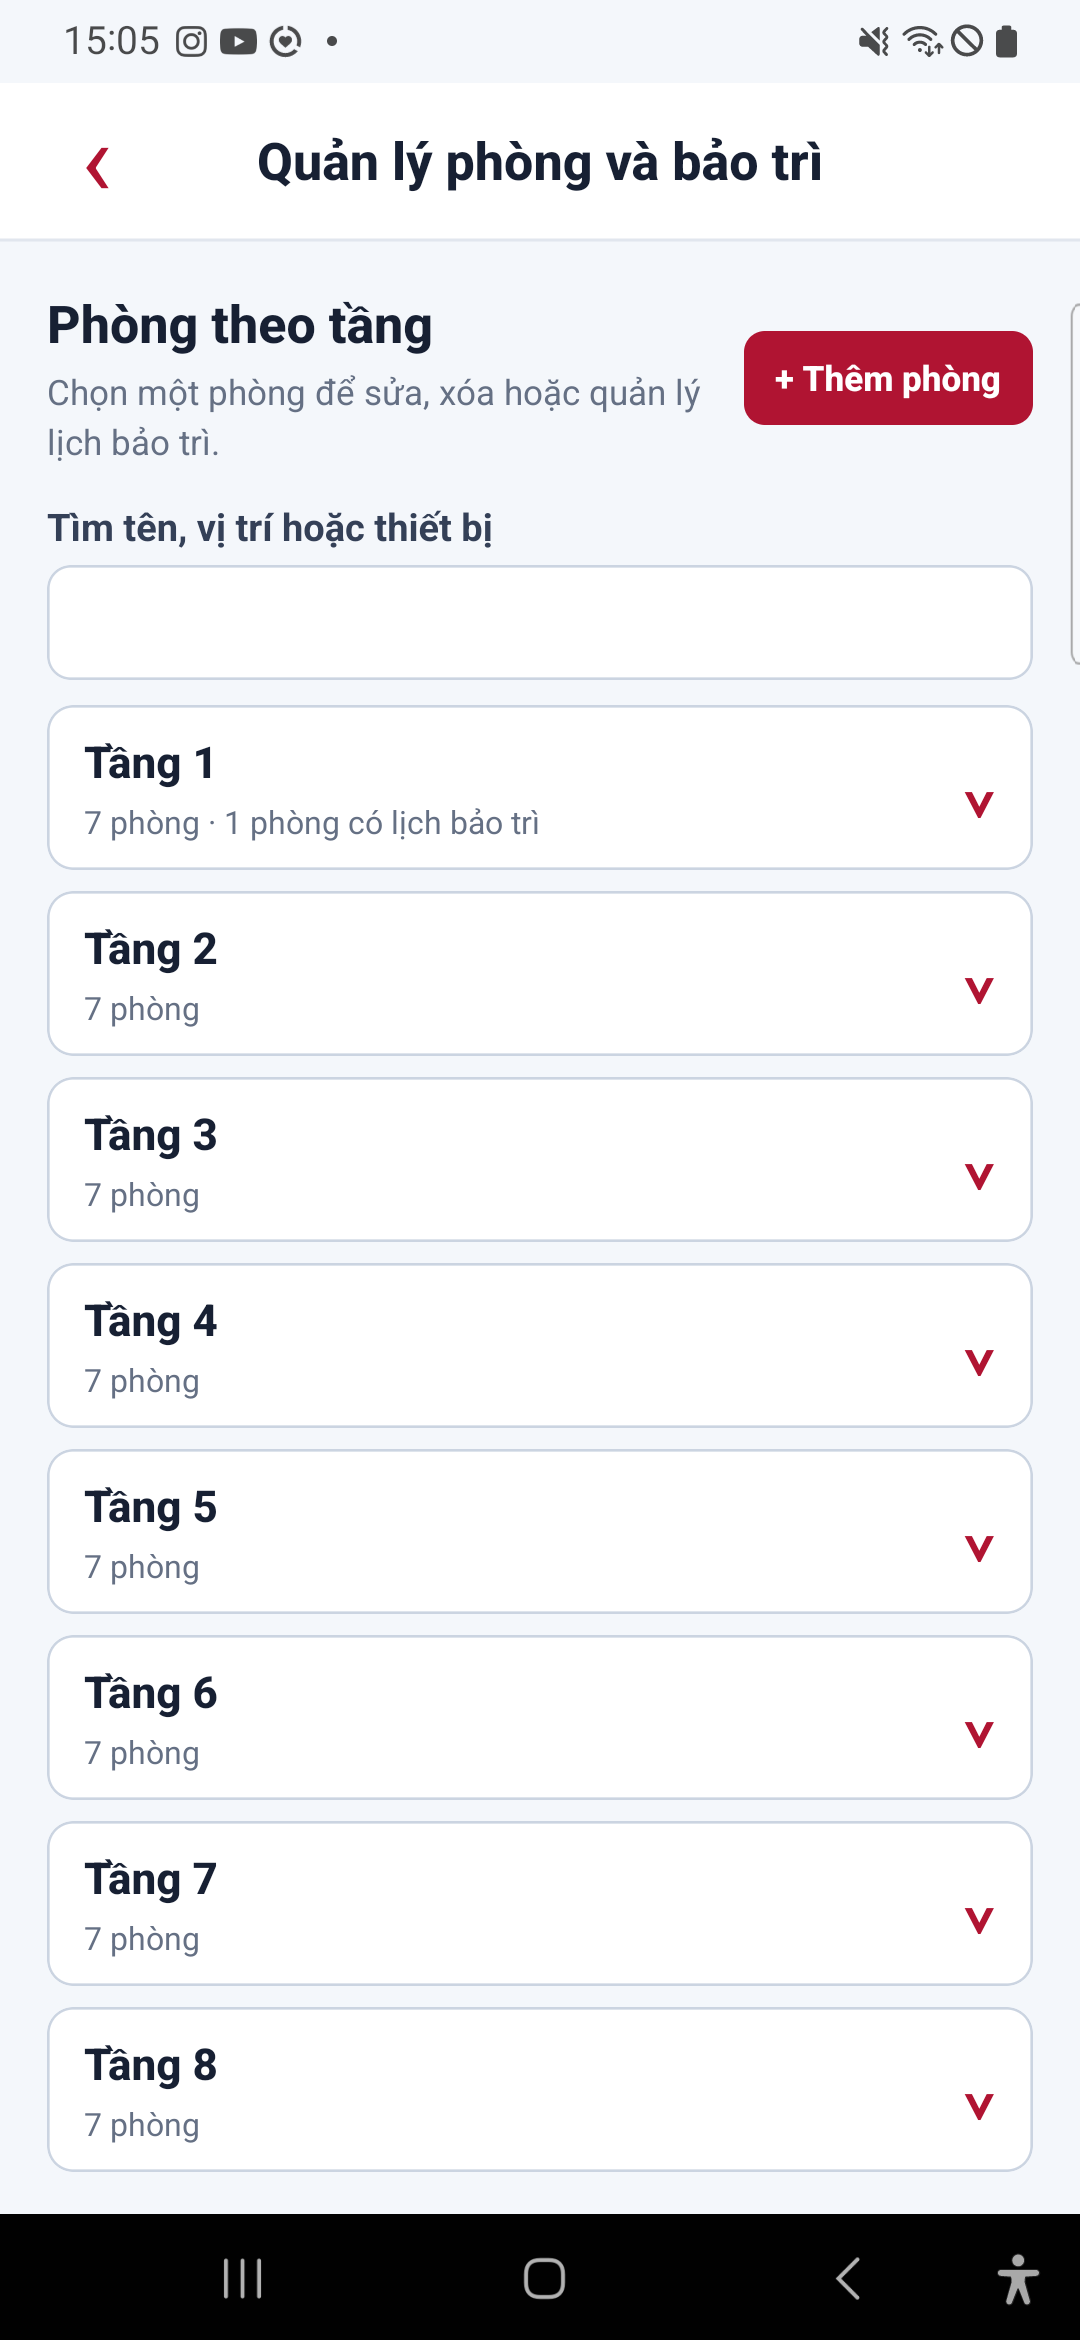
\includegraphics[height=8cm]{Hinhve/quan_ly_phong_theo_tang_hien_tai.png}\hspace{1.2cm}
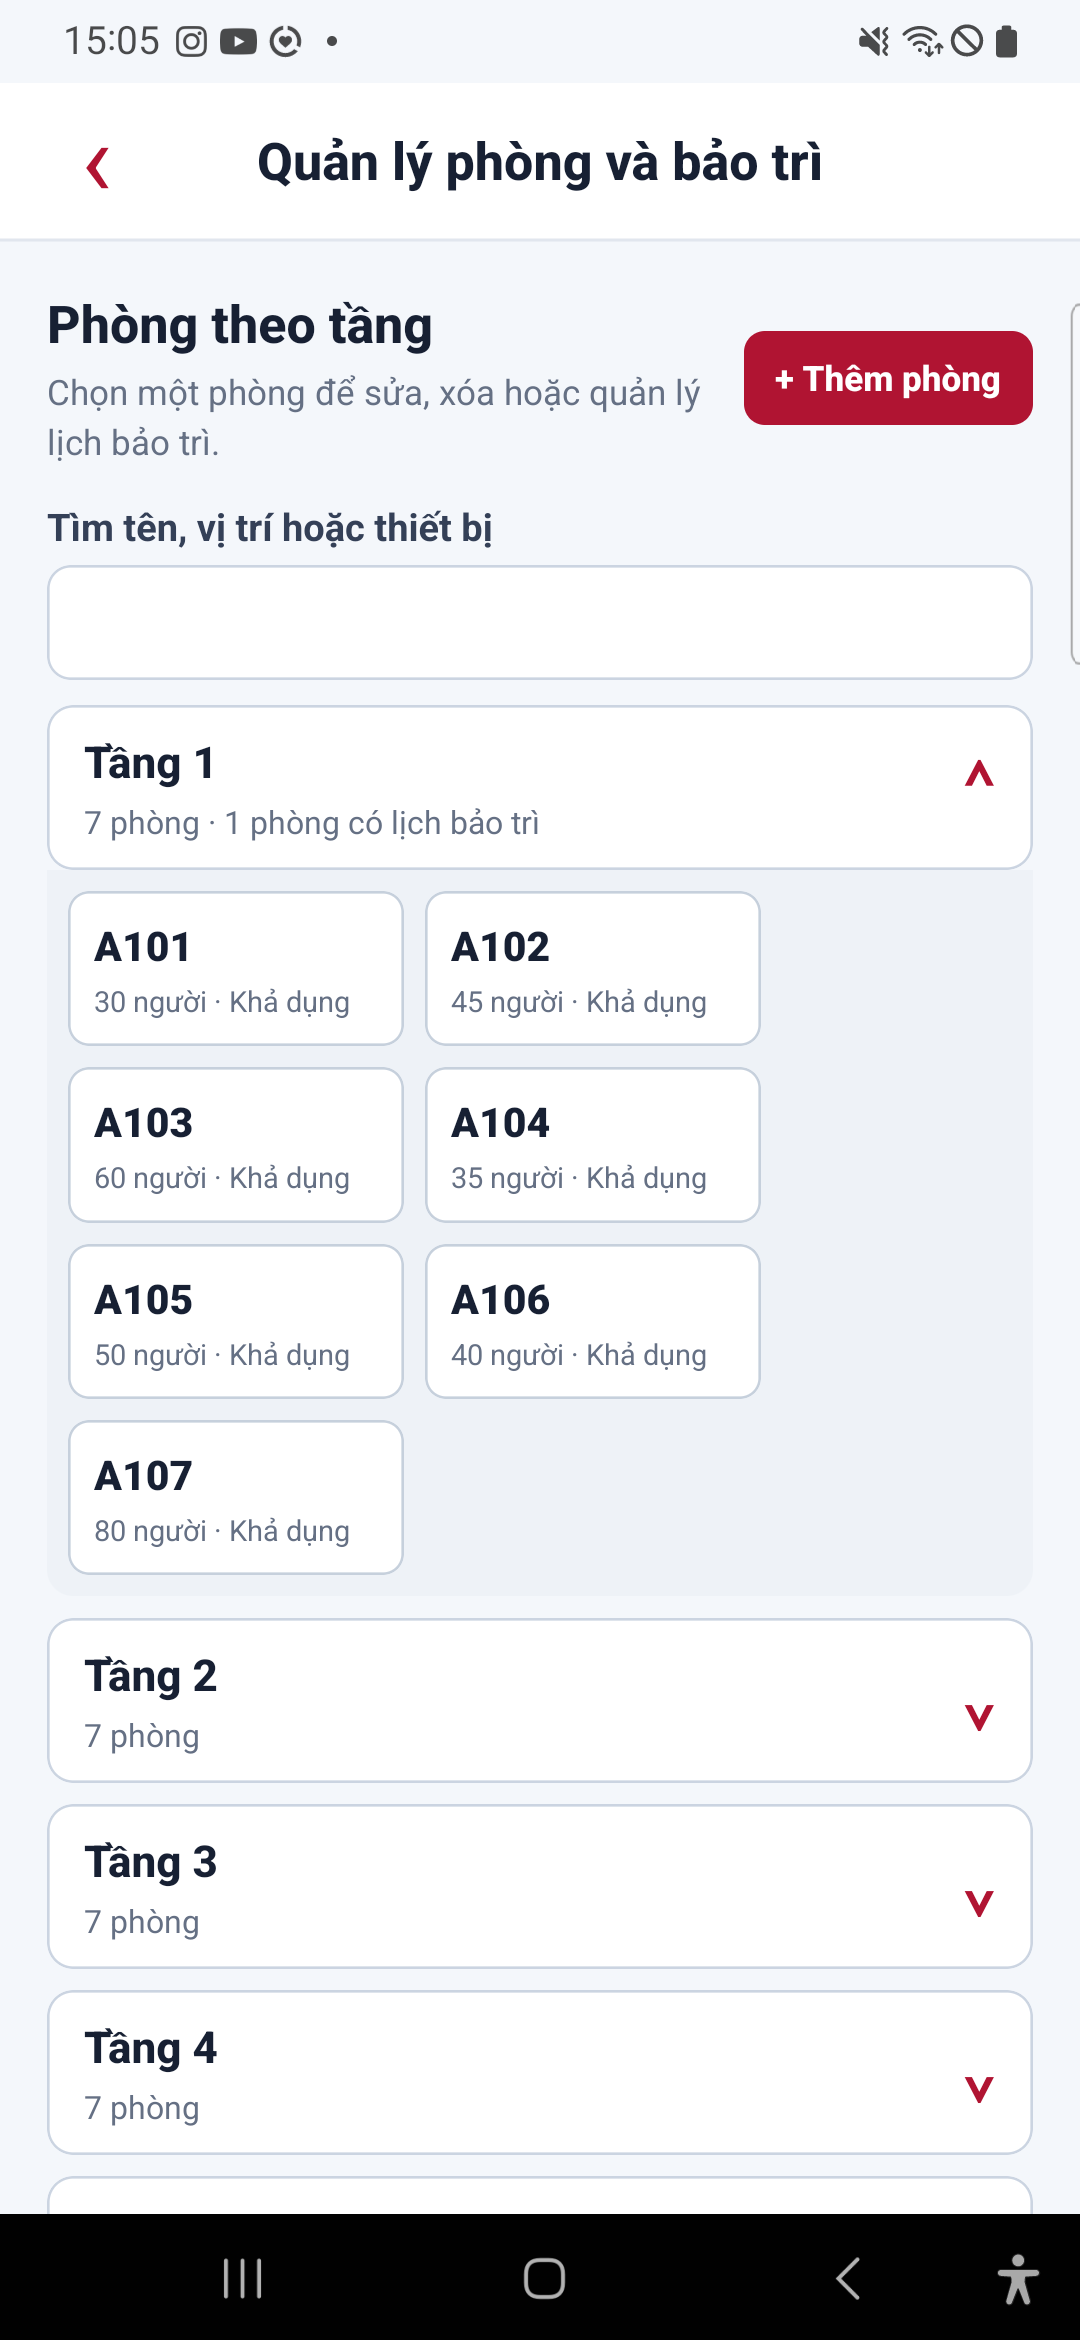
\includegraphics[height=8cm]{Hinhve/phong_tang_mot_hien_tai.png}
\caption{Danh sách tầng và phòng khi mở tầng (trái sang phải)}\label{fig:ui-room-maintenance}
\end{figure}
\subsection{Cấu hình quy tắc đặt phòng}
Hình~\ref{fig:ui-configuration} thể hiện các tham số đặt phòng và công tắc quản trị trên ứng dụng Android. Phần trên gồm cửa sổ đặt trước, hạn mức, hạn hủy/đổi, đệm PIN và ân hạn check-in; phần dưới gồm thông báo hoạt động, tự duyệt phòng thường và nút lưu. Các giá trị được lưu tập trung để dịch vụ nghiệp vụ áp dụng nhất quán. Cấu hình minh họa có min bằng 0, cho phép đặt cùng ngày; giá trị mặc định là 1 ngày. Khi bật tự duyệt, phòng thường được duyệt ngay sau kiểm tra hợp lệ, còn phòng đặc biệt vẫn chờ admin. Kết quả nghiệp vụ được trình bày tại TC07 và TC24.

Form lọc ký tự không phải số; repository vẫn kiểm số nguyên không âm, min không vượt max, hạn mức ít nhất một và quyền admin. Kiểm thử cấu hình xác nhận việc từ chối giá trị vi phạm và thao tác không đủ quyền (TC16).
\begin{figure}[H]\centering
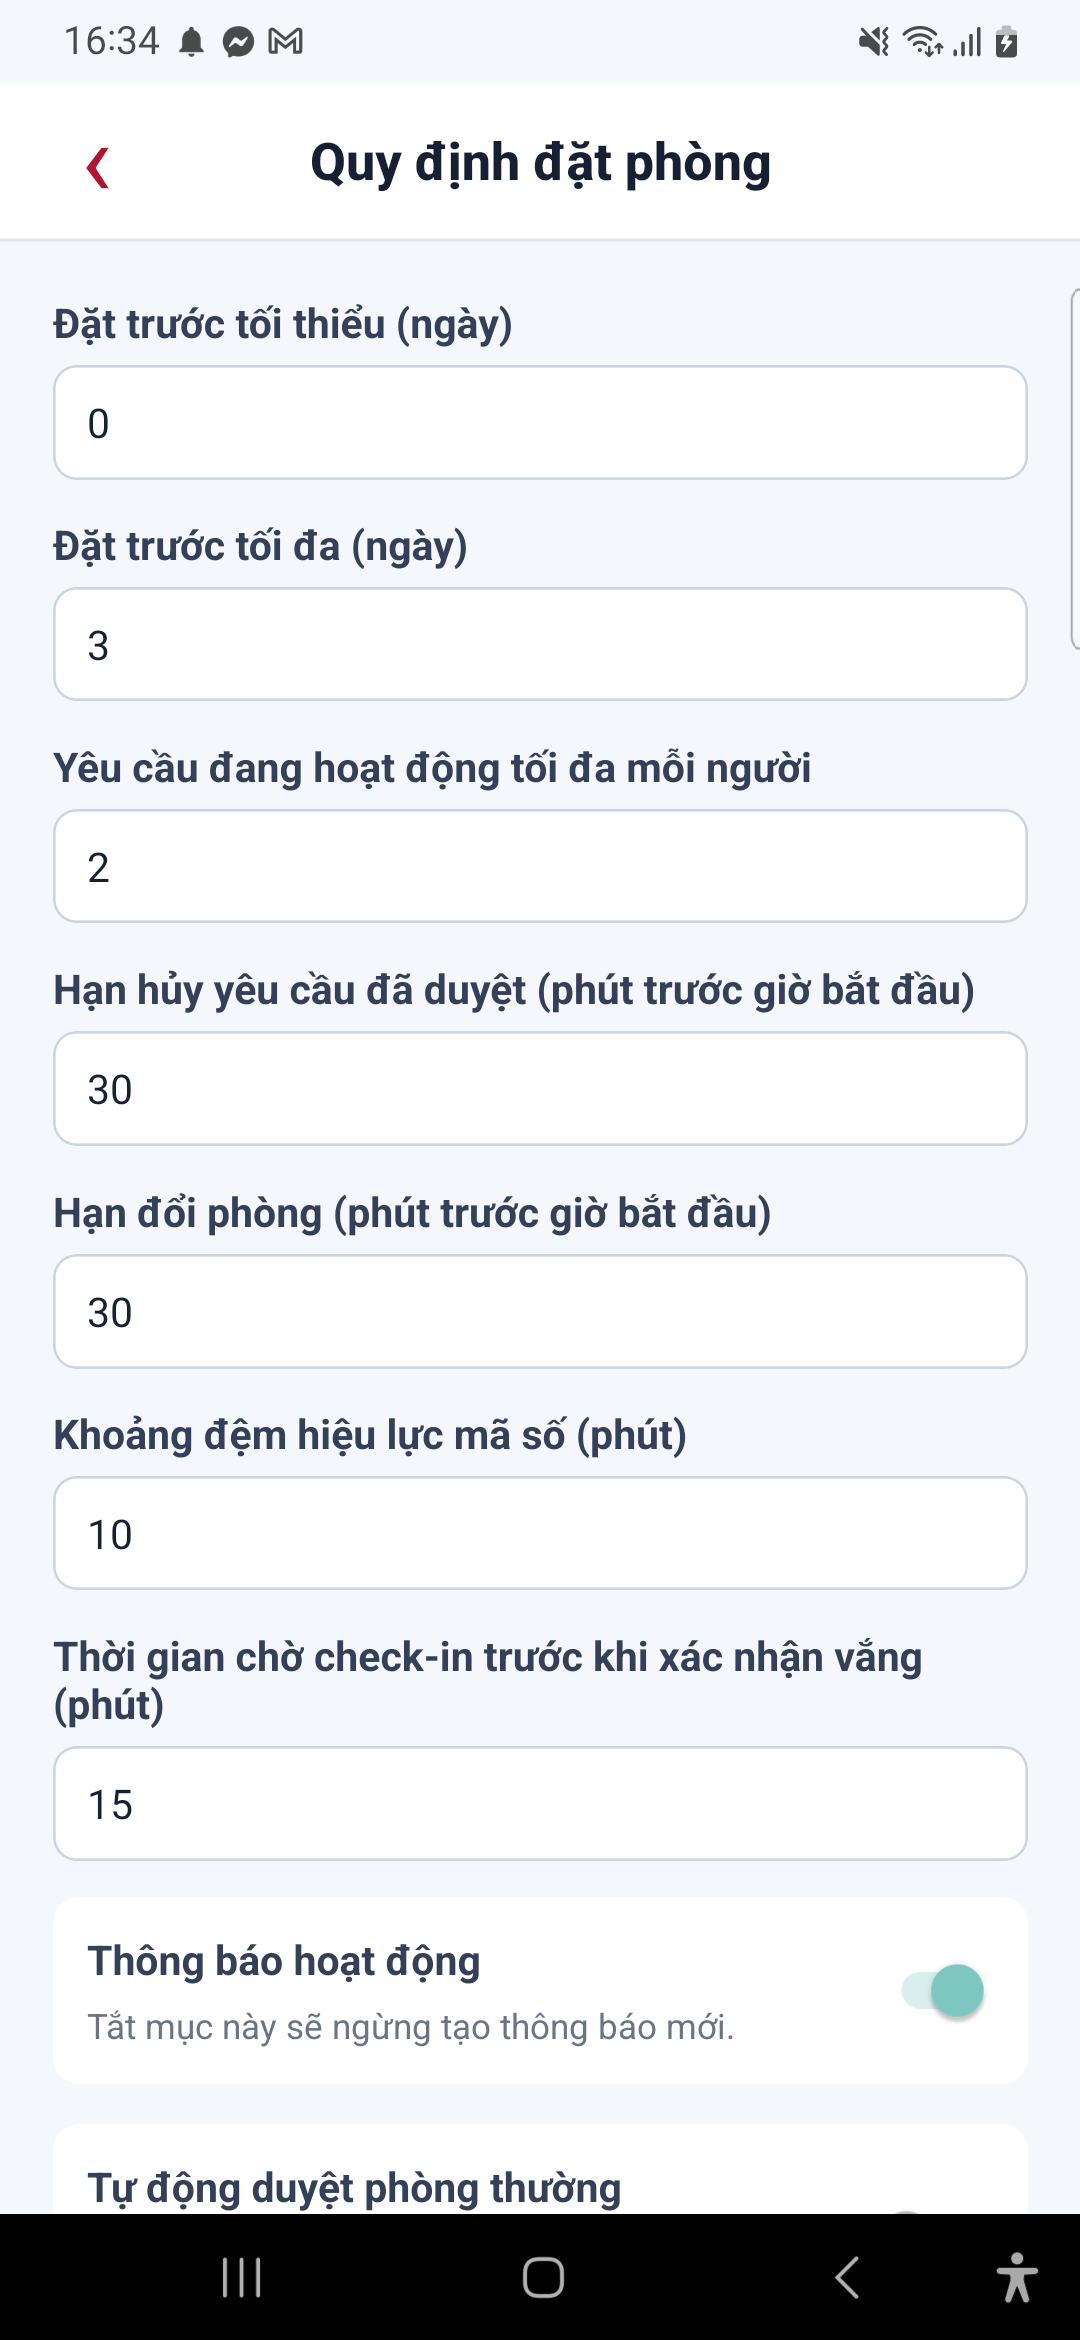
\includegraphics[height=9cm]{Hinhve/cau_hinh_hien_tai.png}\hspace{1cm}
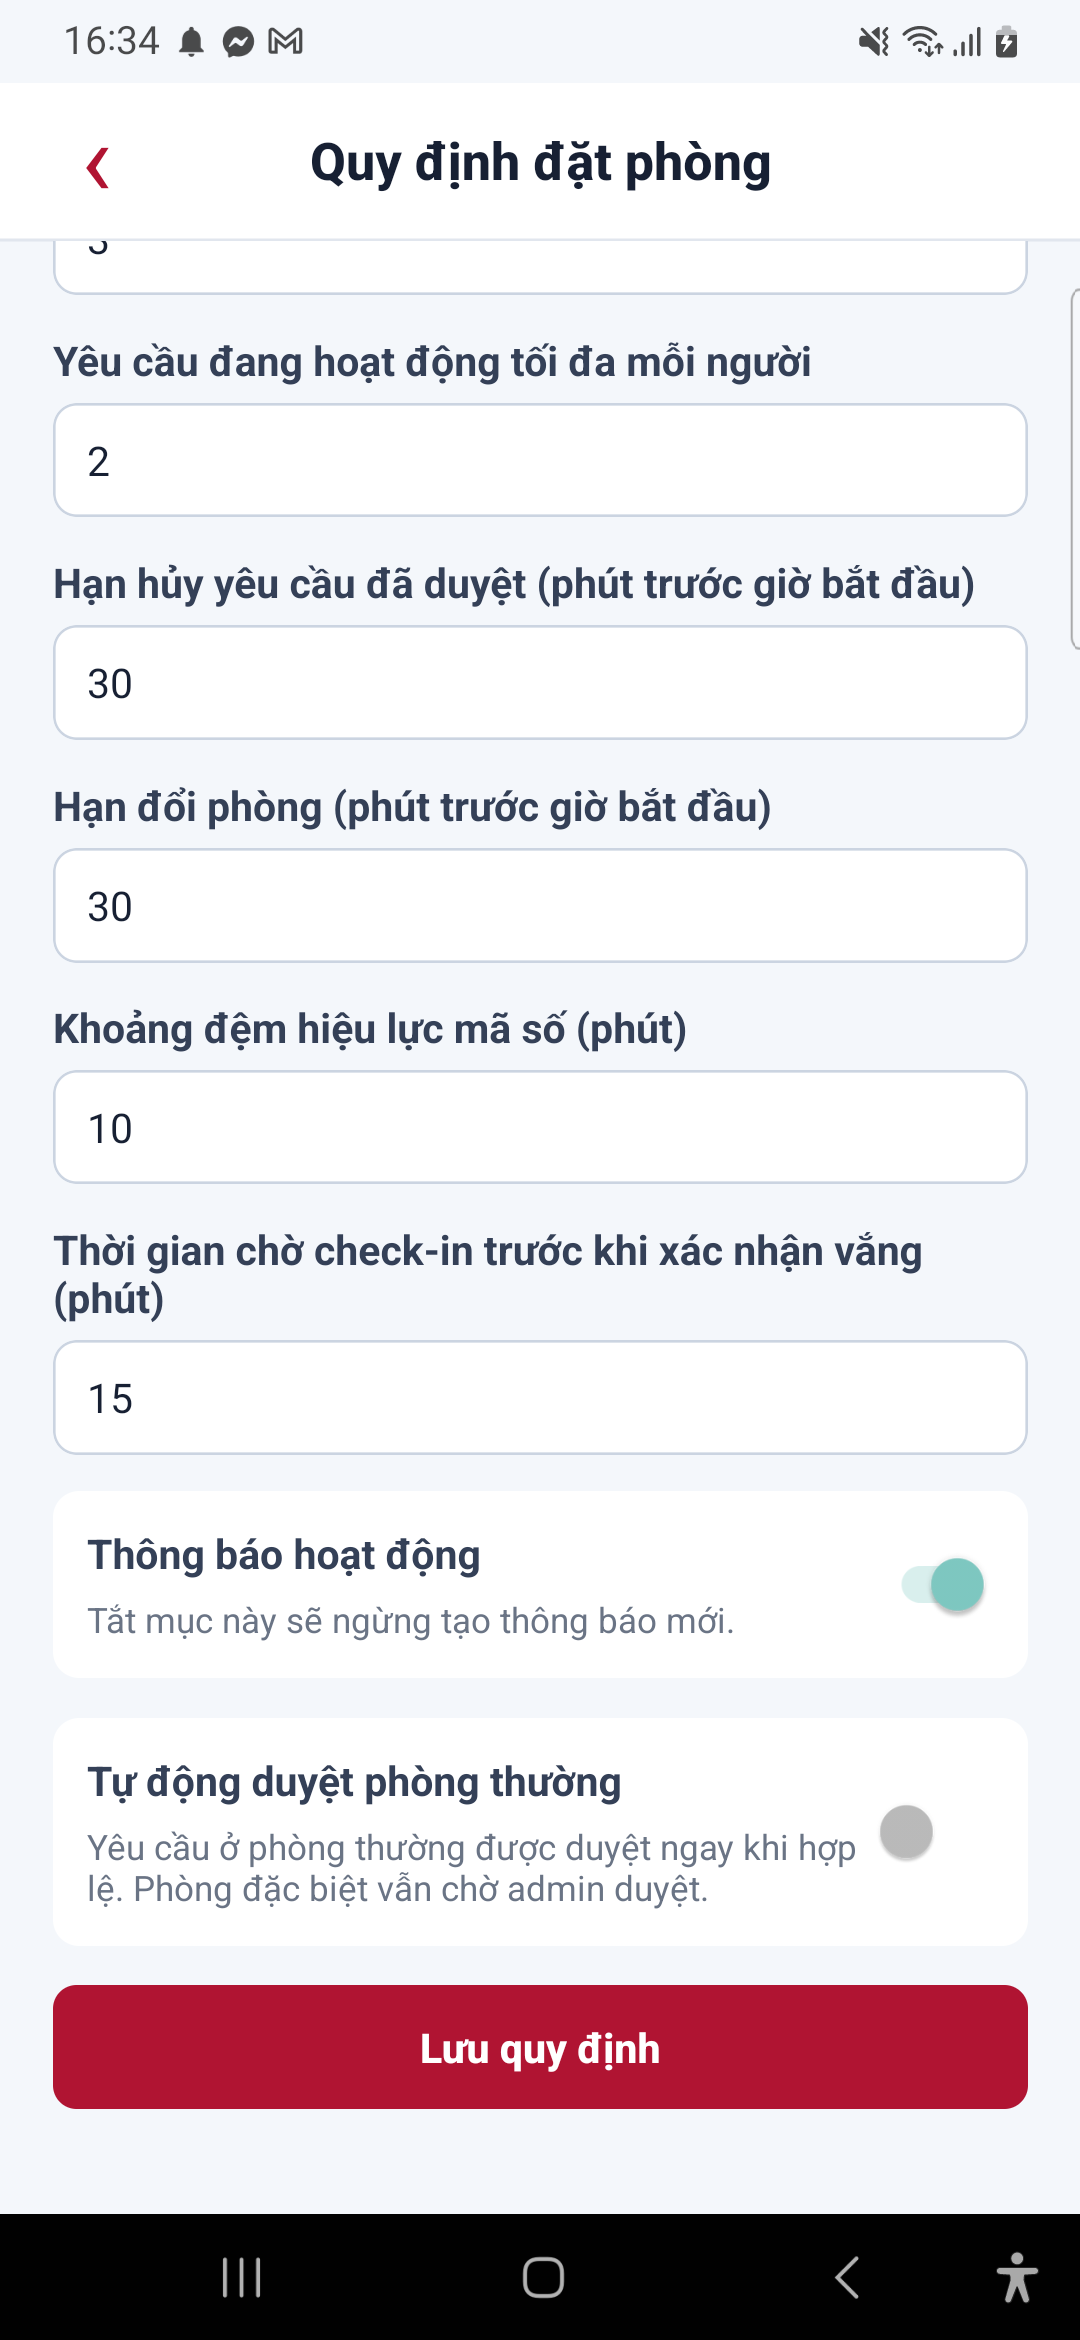
\includegraphics[height=9cm]{Hinhve/cau_hinh_tu_duyet_hien_tai.png}
\caption{Tham số đặt phòng (trái), công tắc thông báo và tự duyệt (phải)}\label{fig:ui-configuration}
\end{figure}
\FloatBarrier

\section{Cấu hình, cài đặt và tái lập bản chạy}
Hình~\ref{fig:deployment} ở Chương~\ref{chap:design} đặt rõ các nơi chạy: APK trên điện thoại, backend/H2 trên máy chủ và kết nối MQTT OneIoT tới khóa. Bảng~\ref{tab:runtime-modes} phân biệt điều kiện sử dụng tương ứng.
{\tabletext\renewcommand{\arraystretch}{1.04}\begin{longtable}{>{\raggedright\arraybackslash}p{\dimexpr0.16\textwidth-2\tabcolsep\relax}>{\raggedright\arraybackslash}p{\dimexpr0.32\textwidth-2\tabcolsep\relax}>{\raggedright\arraybackslash}p{\dimexpr0.52\textwidth-2\tabcolsep\relax}}
\caption{Chế độ chạy, phụ thuộc và phạm vi dữ liệu}\label{tab:runtime-modes}\\
\toprule \textbf{Nhánh} & \textbf{Điều kiện} & \textbf{Hành vi / giới hạn}\\\midrule
\endfirsthead
\multicolumn{3}{l}{\small Chế độ chạy, phụ thuộc và phạm vi dữ liệu (tiếp)}\\
\toprule \textbf{Nhánh} & \textbf{Điều kiện} & \textbf{Hành vi / giới hạn}\\\midrule
\endhead
\bottomrule\endlastfoot
Local & Cờ REST tắt; APK đã có bundle & Đăng nhập và nghiệp vụ dùng Async Storage riêng trên một máy; không cần booking-server. Không tự tải dữ liệu này lên server khi đổi cờ.\\\addlinespace[1.5pt]
REST & Cờ true; backend/URL có thể truy cập từ điện thoại & Repository gọi API, token theo phiên, dữ liệu ở backend. Bản source đang bật nhánh này; URL tunnel trong source là địa chỉ thử nghiệm.\\\addlinespace[1.5pt]
OneIoT & Internet, token Tools trong phiên và khóa gắn với phòng phù hợp & Kết nối MQTT trực tiếp qua native Android, độc lập với cờ REST. PIN được tạo/lưu trước khi gửi; app quản lý metadata gửi lệnh và sự kiện khóa.\\\addlinespace[1.5pt]
\end{longtable}}

\subsection{Cấu hình và dữ liệu khởi tạo}
Cấu hình tại \coderef{code/booking_classroom/src/core/config/runtimeFlags.ts} dùng \code{ENABLE_REMOTE_SYNC=false} cho local, giá trị true cho REST trước khi build; mã nguồn hiện bật REST. Thay đổi cờ hoặc URL được đưa vào JavaScript bundle khi đóng gói lại APK. Local khởi tạo admin/1 và user/2; dữ liệu mẫu chỉ được bổ sung khi kho chưa có, nên cài đè giữ cấu hình và dữ liệu đã lưu.

\subsection{Cài đặt và đóng gói Android}
Tại \code{code/booking_classroom/}, \cmd{npm ci} cài phụ thuộc theo lockfile. Trên Windows, \cmd{npm run build:android:release} tạo bundle, xử lý đường dẫn Unicode qua ổ tạm và gọi Gradle. Trên macOS/Linux, JavaScript được bundle trước khi chạy \cmd{sh ./gradlew assembleRelease} trong thư mục android; cấu hình Release hiện bỏ bước bundle tự động. Quy trình lệnh đầy đủ nằm tại mục~\ref{sec:technical-reproduction} và README gốc repository.

APK đầu ra là \code{android/app/build/outputs/apk/release/app-release.apk}. Sau khi điện thoại cho phép gỡ lỗi USB, cài và mở ứng dụng bằng:
\begin{Verbatim}[fontsize=\small,frame=single,breaklines=true]
adb devices -l
adb install -r android/app/build/outputs/apk/release/app-release.apk
adb shell am start -n com.bookingclassroom/.MainActivity
\end{Verbatim}

Cài đè giữ dữ liệu khi chữ ký tương thích. Bản Release đã đóng gói JavaScript chạy độc lập Metro; chế độ REST cần kết nối backend, còn OneIoT cần mạng và phiên khóa hợp lệ.

\subsection{Backend và kết nối phát triển}
Tại \code{code/booking-server/}, \cmd{mvn spring-boot:run} khởi động dịch vụ cổng 8080 với H2 file. Kết nối qua USB dùng API base URL \code{http://127.0.0.1:8080} và \cmd{adb reverse tcp:8080 tcp:8080}; kết nối Wi-Fi dùng địa chỉ LAN của máy chủ. URL tunnel là địa chỉ tạm thời, phụ thuộc phiên dịch vụ đang chạy.

Bản Debug dùng \cmd{npm start} cho Metro và \cmd{npm run android}; \cmd{adb reverse tcp:8081 tcp:8081} chuyển tiếp cổng Metro qua USB. Cổng 8081 phục vụ JavaScript phát triển, cổng 8080 phục vụ REST. Cơ sở dữ liệu H2 từ xa là lựa chọn bổ sung qua biến BOOKING\_DB; bản local không phụ thuộc cấu hình này.

\FloatBarrier
\chapter{KIỂM THỬ VÀ ĐÁNH GIÁ}\label{chap:testing}
\section{Cấu hình và phương pháp kiểm thử}
{\tabletext\renewcommand{\arraystretch}{1.04}\begin{longtable}{>{\raggedright\arraybackslash}p{\dimexpr0.2\textwidth-2\tabcolsep\relax}>{\raggedright\arraybackslash}p{\dimexpr0.48\textwidth-2\tabcolsep\relax}>{\raggedright\arraybackslash}p{\dimexpr0.32\textwidth-2\tabcolsep\relax}}
\caption{Môi trường, dữ liệu và phạm vi kết quả}\label{tab:test-env}\\
\toprule \textbf{Nhóm kiểm tra} & \textbf{Điều kiện và dữ liệu} & \textbf{Kết quả ghi trong hồ sơ}\\\midrule
\endfirsthead
\multicolumn{3}{l}{\small Môi trường, dữ liệu và phạm vi kết quả (tiếp)}\\
\toprule \textbf{Nhóm kiểm tra} & \textbf{Điều kiện và dữ liệu} & \textbf{Kết quả ghi trong hồ sơ}\\\midrule
\endhead
\bottomrule\endlastfoot
Jest app & Nhánh main; macOS 14.8.9/arm64; Node 22.17.0, Jest 29.7.0. Có 8 suite auth/booking/UI và auto approval; storage/native được mock. & 50/50 ca đạt, gồm 11 ca tự duyệt.\\
Quality suite & Cùng máy và Node/Jest; 17 suite unit, component, integration; mock fetch/native/Async Storage. & 398/398 ca đạt. Unit 259, component 58, integration 81.\\
Quyền thông báo & Bộ bổ sung riêng: 1 suite, 5 ca; mock API 31/33, quyền cho phép/từ chối và native bridge. & 5/5 ca đạt, kiểm logic quyền và native bridge bằng mock.\\
Backend/H2 & 2 ca tích hợp, H2 trong RAM, reset context giữa ca; tài khoản/booking và client cũ thiếu trường mới. & 2/2 ca tích hợp đạt với cơ sở dữ liệu H2 trong RAM.\\
Android thật & Samsung Galaxy M21/SM-M215F; Android 12, API 31; arm64-v8a; MemTotal 3.656.308 KiB (khoảng 3,49 GiB). ADB 37.0.1 qua USB. & APK Release local, package com.bookingclassroom, versionName 1.0/versionCode 1; khởi động độc lập Metro.\\
Kiểm tra tĩnh & TypeScript 5.9.3 và ESLint 8.57.1 theo dependency đã cài; chạy trên cùng source với Jest. & tsc --noEmit và eslint . đều kết thúc mã 0.\\
\end{longtable}}

\subsection{Dữ liệu thử và kiểm soát điều kiện}
Máy thật dùng admin/1, user/2 và tài khoản mới \code{qa0811}, mật khẩu thử 8 ký tự, mã khôi phục 8 chữ số. Hồ sơ thử: \code{RoomHub QA Persist 0811}, \code{qa0811@example.invalid}, đơn vị \code{QA RoomHub 2026}. Không sửa dữ liệu tài khoản cũ; công tắc thông báo được chụp trước/sau và trả về bật. Tài khoản thử được giữ lại để tái lập kết quả.

Bộ kiểm thử chất lượng dùng mốc 08:00 của một ngày giả lập cố định. Các ca đặt phòng dùng ngày tính từ mốc này, trạng thái booking và cấu hình được seed theo từng tình huống. Một số ca chủ động đổi mốc thời gian để kiểm ranh giới tháng, hạn hủy hoặc ân hạn vắng mặt.

Trước mỗi ca liên quan, kho Async Storage giả lập được đặt lại; lượt đặt và cấu hình được khởi tạo theo tình huống. Cách tổ chức này tách các ca có cùng user/phòng, giúp xác định lỗi do điều kiện nghiệp vụ thay vì dữ liệu sót từ ca trước. Dữ liệu có cả hai vai trò, phòng mã số/cơ/thẻ, lượt chờ/đã duyệt/hủy và thời điểm nằm trong/ngoài khoảng cho phép.

Hai ca Spring Boot dùng HTTP qua TestRestTemplate và H2 trong RAM. Ca thứ nhất đi qua hồ sơ, chuỗi booking, duyệt, gắn khóa, lưu metadata PIN và tách dữ liệu theo tài khoản; ca thứ hai kiểm tự duyệt và client cũ không gửi hai trường mới. Môi trường Spring được khởi tạo lại sau mỗi phương thức để tách dữ liệu giữa hai ca; mỗi ca kiểm tra một chuỗi nhiều thao tác HTTP.

\Needspace{6\baselineskip}
\subsection{Các phương pháp kiểm thử}
Quy trình kết hợp kiểm thử logic, giao diện, API, tích hợp và vận hành thiết bị. Bảng~\ref{tab:evidence-levels} trình bày nội dung và vai trò của từng phương pháp.
{\tabletext\renewcommand{\arraystretch}{1.04}\begin{longtable}{>{\raggedright\arraybackslash}p{\dimexpr0.20\textwidth-2\tabcolsep\relax}>{\raggedright\arraybackslash}p{\dimexpr0.43\textwidth-2\tabcolsep\relax}>{\raggedright\arraybackslash}p{\dimexpr0.37\textwidth-2\tabcolsep\relax}}
\caption{Phương pháp và vai trò trong kiểm thử}\label{tab:evidence-levels}\\
\toprule \textbf{Phương pháp} & \textbf{Nội dung kiểm tra} & \textbf{Vai trò}\\\midrule
\endfirsthead
\multicolumn{3}{l}{\small Phương pháp và vai trò trong kiểm thử (tiếp)}\\
\toprule \textbf{Phương pháp} & \textbf{Nội dung kiểm tra} & \textbf{Vai trò}\\\midrule
\endhead
\bottomrule\endlastfoot
Unit/component & Quy tắc dữ liệu, phân quyền, thay đổi state và phản hồi giao diện với đầu vào xác định. & Kiểm tra từng thành phần và phát hiện lỗi nghiệp vụ/giao diện.\\
Integration local & Chuỗi thao tác giữa service, dữ liệu booking, quyền, PIN và thông báo; mô phỏng sự kiện khóa. & Kiểm tra sự phối hợp giữa các module và các nhánh ngoại lệ.\\
Hợp đồng API & Method/path, payload, token Bearer, mã lỗi và cấu trúc phản hồi. & Giữ thống nhất giao tiếp giữa ứng dụng và backend.\\
Spring Boot/H2 & Luồng HTTP, quyền theo token, ghi/đọc dữ liệu và tương thích cấu hình. & Kiểm tra nghiệp vụ server và giao dịch lưu trữ.\\
Android và SmartLock & Cài/khởi động, đăng nhập, đặt/duyệt phòng, cấp PIN, kết nối khóa, sự kiện và thông báo. & Xác nhận các luồng sử dụng và tích hợp app/khóa trong vận hành thực tế.\\
Ảnh giao diện & Màn hình, thao tác và trạng thái kết quả của các chức năng. & Minh họa trải nghiệm người dùng cùng kết quả thực nghiệm.\\
\end{longtable}}

Các bộ kiểm thử có thể cùng kiểm một quy tắc ở nhiều mức, nên tổng số ca không tương ứng với số chức năng độc lập. Chỉ tiêu độ phủ mã được tách khỏi kết quả đạt/không đạt của các ca chức năng.

\section{Ca kiểm thử chức năng và kết quả thực tế}
Bảng~\ref{tab:cases} tổng hợp ca nghiệp vụ; Bảng~\ref{tab:android-cases} ghi nhận thao tác Android \cite{qualityreport,devicereport,currenttests}. Nhóm xác nhận hoàn thành các chức năng app--SmartLock qua vận hành thực tế \cite{systemacceptance}.
{\tabletext\renewcommand{\arraystretch}{1.04}\begin{longtable}{>{\raggedright\arraybackslash}p{\dimexpr0.23\textwidth-2\tabcolsep\relax}>{\raggedright\arraybackslash}p{\dimexpr0.26\textwidth-2\tabcolsep\relax}>{\raggedright\arraybackslash}p{\dimexpr0.35\textwidth-2\tabcolsep\relax}>{\raggedright\arraybackslash}p{\dimexpr0.16\textwidth-2\tabcolsep\relax}}
\caption{Ca tiêu biểu, kỳ vọng, thực tế và kết luận}\label{tab:cases}\\
\toprule \textbf{ID / dữ liệu} & \textbf{Kỳ vọng} & \textbf{Kết quả thực tế} & \textbf{Kết luận}\\\midrule
\endfirsthead
\multicolumn{4}{l}{\small Ca tiêu biểu, kỳ vọng, thực tế và kết luận (tiếp)}\\
\toprule \textbf{ID / dữ liệu} & \textbf{Kỳ vọng} & \textbf{Kết quả thực tế} & \textbf{Kết luận}\\\midrule
\endhead
\bottomrule\endlastfoot
TC01: admin/1, user/2; user/wrong & Hợp lệ mở đúng vai trò; sai không tạo phiên UI. & Sai mật khẩu báo lỗi; admin/user hợp lệ mở đúng dashboard trên Android. & Đạt: Android và mock.\\
TC02: lịch phòng chồng giờ, bảo trì và vượt hạn mức & Từ chối tạo; khoảng liền kề không chồng. & Từ chối trùng phòng/user, bảo trì và vượt hạn mức; nhận hai khoảng chạm biên. & Đạt: quality.\\
TC03: đã duyệt, phòng PIN, đúng user/quyền & Mã 7 số; hiệu lực theo đệm; chặn mã thứ hai khi PIN trước chưa thu hồi. & PIN đủ 7 số, hiệu lực đúng đệm; chặn mã thứ hai khi PIN cũ chưa thu hồi. & Đạt: local/mock.\\
TC04: HTTP 401 / JSON hỏng / mất mạng & Xóa token với 401; hiển thị lỗi phù hợp; không fallback local. & 401 xóa token; JSON hỏng/mất mạng báo lỗi; vẫn giữ nguồn REST. & Đạt: HTTP mock.\\
TC05: request vượt 12 giây giả lập & Abort request và thông báo timeout; clear timer. & Đồng hồ giả lập tới 12 giây: request bị abort, trả lỗi timeout và dọn timer. & Đạt: timer giả lập.\\
TC06: thông báo admin khi user đang đăng nhập & Lưu đúng người nhận; không hiện nhầm banner. & Thông báo được lưu cho admin; khi user đang đăng nhập, banner dành cho admin không xuất hiện. & Đạt: quality.\\
TC07: bật tự duyệt; phòng thường/phòng đặc biệt & Thường APPROVED, special PENDING; vẫn kiểm booking rules. & Phòng thường chuyển APPROVED; phòng đặc biệt giữ PENDING; các yêu cầu vi phạm quy tắc vẫn bị chặn. & Đạt: 11 ca app.\\
TC08: từ chối thông báo; phân biệt API 31 và 33+ & UI vẫn dùng được; quyền bị chặn không gửi native trên API 33+. & API 33 giả lập chặn native khi bị từ chối quyền; API 31 tắt thông báo vẫn lưu hồ sơ và hiện banner. & Đạt: mock/API 31.\\
TC09: lưu hồ sơ qa0811, force-stop và mở lại & App mở không cần Metro; đăng nhập lại đọc đúng dữ liệu đã lưu. & Sau force-stop, app mở với PID mới và yêu cầu đăng nhập; họ tên, email và đơn vị giữ nguyên. & Đạt: Android.\\
TC10: ứng dụng kết nối và sử dụng SmartLock & App kết nối OneIoT, cấp mã và thao tác khóa đúng luồng nghiệp vụ. & Theo kết quả vận hành nhóm xác nhận, app kết nối OneIoT, cấp mã và thực hiện luồng sử dụng SmartLock. & Đạt: nhóm nghiệm thu.\\
\end{longtable}}

\subsection{Kiểm thực tế trên Android}
D01--D06 dùng APK local mục 5.1, có ảnh PNG/XML và \code{persistence-result.json}. Hồ sơ: \code{docs/reports/final/LTUD/minh_chung/kiem_thu/} \cite{currenttests}.
{\tabletext\renewcommand{\arraystretch}{1.04}\begin{longtable}{>{\raggedright\arraybackslash}p{\dimexpr0.30\textwidth-2\tabcolsep\relax}>{\raggedright\arraybackslash}p{\dimexpr0.26\textwidth-2\tabcolsep\relax}>{\raggedright\arraybackslash}p{\dimexpr0.44\textwidth-2\tabcolsep\relax}}
\caption{Bước thử, kỳ vọng và quan sát trên máy thật}\label{tab:android-cases}\\
\toprule \textbf{ID / bước và dữ liệu} & \textbf{Kỳ vọng} & \textbf{Thực tế / minh chứng / kết luận}\\\midrule
\endfirsthead
\multicolumn{3}{l}{\small Kiểm thực tế trên Android (tiếp)}\\
\toprule \textbf{ID / bước và dữ liệu} & \textbf{Kỳ vọng} & \textbf{Thực tế / minh chứng / kết luận}\\\midrule
\endhead
\bottomrule\endlastfoot
D01 -- Đăng nhập user với mật khẩu wrong. & Báo lỗi; vẫn ở trang đăng nhập. & Hiện Sai tài khoản hoặc mật khẩu; không mở dashboard. Ảnh/XML 04-wrong-password-rejected. Đạt.\\
D02 -- Đăng nhập user/2, đăng xuất rồi admin/1. & Phân biệt giảng viên và quản trị viên. & UI hiện GIẢNG VIÊN và QUẢN TRỊ; menu tương ứng. Minh chứng 07-user-dashboard-clean và 45-admin-dashboard. Đạt.\\
D03 -- Đăng ký qa0811 với hai mật khẩu trùng, email thử và mã khôi phục hợp lệ; đăng nhập. & Tạo tài khoản giảng viên; đọc được hồ sơ đã nhập. & Thông báo đăng ký thành công, dashboard đúng user, hồ sơ ban đầu đúng. Minh chứng 13, 17, 19. Đạt.\\
D04 -- Trong hồ sơ qa0811, thay họ tên bằng một dấu cách rồi lưu. & Chặn giá trị trống sau trim. & Hiện Họ và tên không được để trống; sửa lại dữ liệu hợp lệ lưu được. Minh chứng 23-profile-validation-error và 31. Đạt.\\
D05 -- Tắt Hiện thông báo trong Android; mở app, lưu hồ sơ thử. & Thao tác và phản hồi trong app vẫn dùng được. & Cài đặt ghi Thông báo từ ứng dụng này bị chặn; app vẫn báo đã lưu và hiện banner. Minh chứng 28, 30; bật lại ở 39. Đạt trên API 31.\\*
D06 -- Lưu ba trường hồ sơ mục 5.1; force-stop, kiểm tiến trình dừng, mở lại, đăng nhập qa0811 và đọc hồ sơ. & Mở độc lập Metro; dữ liệu đã lưu giữ nguyên. & Không còn tiến trình sau dừng, PID đổi khi mở; ba trường trước/sau bằng nhau. Minh chứng 31, 32, 37 và JSON đối chiếu. Đạt với hồ sơ local.\\
\end{longtable}}

Trên Android API 31, D05 kiểm tra công tắc thông báo hệ thống. Bộ bổ sung mô phỏng API 33 để kiểm logic xin quyền, từ chối quyền và hiển thị banner; D06 kiểm tra dữ liệu hồ sơ trước và sau khi đóng/mở ứng dụng.

\subsection{Ca chi tiết theo nhóm nghiệp vụ}
Các ca TC11--TC24 làm rõ đầu vào và ngoại lệ của các luồng còn lại. TC11--TC23 tổng hợp kết quả từ bộ quality 398 ca đạt với storage/native được mô phỏng \cite{currenttests}; TC24 dùng kết quả tích hợp H2 \cite{qualityreport}. Danh mục tệp kiểm thử và kết quả gốc được lưu trong hồ sơ minh chứng. Các ca Android được trình bày riêng ở Bảng~\ref{tab:android-cases}.
{\tabletext\renewcommand{\arraystretch}{1.04}\begin{longtable}{>{\raggedright\arraybackslash}p{\dimexpr0.31\textwidth-2\tabcolsep\relax}>{\raggedright\arraybackslash}p{\dimexpr0.31\textwidth-2\tabcolsep\relax}>{\raggedright\arraybackslash}p{\dimexpr0.38\textwidth-2\tabcolsep\relax}}
\caption{Ca nghiệp vụ chi tiết và kết quả}\label{tab:cases-detail}\\
\toprule \textbf{ID / bước và dữ liệu} & \textbf{Kỳ vọng} & \textbf{Kết quả thực tế / kết luận}\\\midrule
\endfirsthead
\multicolumn{3}{l}{\small Ca nghiệp vụ chi tiết và kết quả (tiếp)}\\
\toprule \textbf{ID / bước và dữ liệu} & \textbf{Kỳ vọng} & \textbf{Kết quả thực tế / kết luận}\\\midrule
\endhead
\bottomrule\endlastfoot
TC11 -- Tạo lượt hợp lệ với tự duyệt tắt; kiểm thông báo sau ghi. & PENDING; admin nhận thông báo yêu cầu mới, mục đích được chuẩn hóa. & Lượt được lưu PENDING với mục đích đã bỏ khoảng trắng thừa; thông báo yêu cầu mới được ghi cho admin. Đạt (quality).\\
TC12 -- Dịch ngày đặt 0/1/2/3/4 ngày khi cấu hình 1--3; sau đó seed cửa sổ 2--5 ngày. & Chỉ 1/2/3 hợp lệ theo mặc định; với cấu hình mới, ngày 1 bị chặn và ngày 5 được nhận. & Với cửa sổ 1--3, ngày 0/4 bị từ chối và ngày 1/2/3 được nhận; đổi sang 2--5 chặn ngày 1, nhận ngày 5. Đạt (quality).\\
TC13 -- Yêu cầu PENDING, phòng cơ/thẻ, người khác, quyền chưa cấp hoặc booking đã kết thúc thử tạo PIN. & Từ chối theo trạng thái, loại phòng, người đặt/quyền và thời hạn tương ứng. & Các trường hợp sai trạng thái, sai loại khóa, khác chủ/quyền hoặc đã hết giờ đều trả lỗi tương ứng và không tạo PIN. Đạt (quality).\\
TC14 -- Thu hồi quyền user--phòng rồi tạo PIN; cấp lại quyền khi cần. & Sau thu hồi, user bị chặn tự tạo PIN; cấp lại tái sử dụng bản ghi quyền. Việc tạo mã còn phải thỏa điều kiện booking/PIN riêng. & Sau thu hồi, kiểm tra quyền trả false và tạo PIN bị chặn; cấp lại kích hoạt cùng định danh bản ghi quyền. Đạt (quality).\\
TC15 -- Đổi booking sang phòng PIN khác khi khóa duy nhất vẫn gắn phòng cũ. & Ghi phòng mới, đánh dấu PIN cũ thu hồi; không tạo mã cho phòng chưa gắn SmartLock. & Lượt trỏ sang phòng mới; PIN cũ có dấu thu hồi và quyền phòng mới được cấp. Tạo PIN tại phòng chưa gắn khóa trả lỗi. Đạt (quality).\\
TC16 -- User thử tạo phòng/tài khoản hoặc lưu cấu hình quản trị. & Service từ chối; không dựa riêng vào việc menu bị ẩn. & User nhận lỗi không đủ quyền khi ghi phòng, tạo tài khoản hoặc cập nhật cấu hình; dữ liệu quản trị không được ghi. Đạt (quality).\\
TC17 -- Tài khoản bị khóa đăng nhập; đổi/khôi phục mật khẩu với input sai và đúng. & Không tạo phiên cho tài khoản khóa; mật khẩu cũ sai sau đổi; mã khôi phục sai bị từ chối. & Tài khoản khóa không tạo phiên; sau đổi, mật khẩu cũ không còn hợp lệ; mã khôi phục sai bị từ chối. Đạt (quality).\\
TC18 -- Admin tạo/sửa/xóa phòng; thử xóa khi còn booking hoạt động và thử đọc lại phòng mẫu đã xóa. & Chuẩn hóa dữ liệu, giữ định danh khi sửa, chặn xóa khi còn lượt hoạt động; phòng mẫu đã xóa không tự tái xuất hiện. & Sửa phòng giữ định danh; xóa phòng có lượt hoạt động bị chặn. Phòng mẫu đã xóa không xuất hiện lại khi đọc danh mục. Đạt (quality).\\
TC19 -- Đề xuất/đề xuất lại lịch nhận chìa; sai lượt phản hồi; thiếu địa điểm; nhập người nhận hộ. & Hai bên xác nhận đúng lượt; admin phải có địa điểm; lịch tương lai trước giờ dùng; người nhận hộ có đủ tên và mã. & Lịch chuyển AGREED khi hai bên chấp nhận đúng lượt; lịch sử đề xuất và người nhận hộ được lưu. Sai lượt/thiếu địa điểm trả lỗi. Đạt (quality).\\
TC20 -- Đổi phòng sai loại khóa, thiếu sức chứa/thiết bị, phòng đã bị giữ hoặc quá hạn. & Chặn thay thế không phù hợp; chỉ đổi lượt đã duyệt khi đủ điều kiện và ghi lịch sử. & Phòng sai loại khóa, thiếu sức chứa/thiết bị, đã bị giữ hoặc quá hạn bị từ chối; ca hợp lệ cập nhật phòng và lịch sử. Đạt (quality).\\
TC21 -- Đặt chuỗi tuần với một tuần sau xung đột; sửa/hủy chuỗi theo người sở hữu và hạn chót. & Không tạo dở chuỗi khi một lượt xung đột; chỉ sửa lượt tương lai PENDING; hủy kiểm toàn bộ lượt chịu cutoff. & Một tuần xung đột làm thao tác tạo/sửa bị từ chối toàn bộ; không ghi dở chuỗi. Sửa và hủy chỉ tác động các lượt đủ điều kiện. Đạt (quality).\\
TC22 -- Đánh dấu no-show trước/tại ngưỡng 15 phút hoặc sau khi đã có check-in. & Chỉ admin, đủ ân hạn và chưa có bằng chứng có mặt; no-show giải phóng khung giờ, đánh dấu PIN thu hồi trong dữ liệu. & Trước ân hạn hoặc đã check-in bị từ chối; đúng ngưỡng được ghi NO\_SHOW, đánh dấu PIN thu hồi và cho phép đặt lại khung giờ. Đạt (quality).\\
TC23 -- Chủ lượt APPROVED đang sử dụng gửi ghi chú hoặc báo sự cố. & Ghi chú gửi admin nhưng không tạo maintenance; yêu cầu bảo trì qua bước lên lịch mới chặn phòng. & Ghi chú tạo thông báo admin, kho bảo trì không tăng; yêu cầu bảo trì chỉ sinh lịch chặn phòng sau khi admin lên lịch. Đạt (quality).\\
TC24 -- Client cũ PUT cấu hình/phòng thiếu autoApprovalEnabled hoặc requiresApproval. & Giữ giá trị đã có; phòng thường tự duyệt, phòng đặc biệt vẫn PENDING tới khi admin xử lý. & Cập nhật thiếu hai cờ mới giữ nguyên giá trị đã lưu; phòng thường APPROVED, phòng đặc biệt PENDING. Đạt theo hồ sơ 2/2 ca H2.\\
\end{longtable}}

Vòng đời PIN được quản lý bằng revokedAt và trạng thái booking. Quyền user--phòng là bản ghi riêng; thao tác hủy/no-show cập nhật lượt đặt và PIN tương ứng. Việc tạo PIN tiếp theo tuân theo trạng thái thu hồi của mã hiện có.

\subsection{Truy vết một chuỗi kiểm thử tích hợp}
Chuỗi tích hợp phòng PIN bắt đầu bằng đăng ký tài khoản gv.an, gắn khóa cho room-a101 và tạo booking 09:00--11:00 vào ngày kế tiếp mốc giả lập. Sau admin duyệt, test xác nhận quyền phòng; tạo PIN khi OneIoT chưa kết nối phải có mã bảy số nhưng chưa có lockDeliveredAt. Khi mock kết nối chuyển online, test kiểm gửi đúng phòng, ID mật khẩu, epoch từ 08:50 tới 11:10 và không gửi lại mã đã ghi nhận gửi.

Bước tiếp theo đưa bản tin traitUnlockTempPwd lúc 08:55 và traitLocked lúc 10:58 vào parser để kiểm checkedInAt/checkedOutAt. Sau có check-in, yêu cầu đánh dấu vắng mặt phải bị từ chối. Chuỗi này kết nối các module booking, quyền phòng, PIN, MQTT adapter và thông báo; lớp mạng/native được mock để kiểm soát đầu vào và tái hiện các tình huống kết nối.

Ca riêng giả lập MQTT timeout, kiểm lockDeliveryError và lần kết nối sau gửi thành công phải xóa lỗi; qua đó kiểm trạng thái chờ/lỗi và gửi lại trong dữ liệu ứng dụng.

Kết quả từng bộ được lưu dưới dạng JSON và nhật ký; ảnh PNG/XML ghi nhận thao tác Android và trạng thái dữ liệu trước/sau. Các lệnh tái lập tập trung tại mục~\ref{sec:test-reproduction}; hồ sơ chi tiết được dẫn trong tài liệu \cite{currenttests}.

\Needspace{18\baselineskip}
\section{Phạm vi đánh giá chất lượng định lượng}
Đánh giá hiện tại tập trung vào tính đúng chức năng và khả năng vận hành Android--SmartLock. Các phép đo thời gian khởi động, độ trễ đầu cuối và ổn định dài hạn không được thực hiện trong đợt đánh giá chức năng; Bảng~\ref{tab:metrics} nêu điều kiện đo và phạm vi tương ứng.
{\tabletext\renewcommand{\arraystretch}{1.04}\begin{longtable}{>{\raggedright\arraybackslash}p{\dimexpr0.23\textwidth-2\tabcolsep\relax}>{\raggedright\arraybackslash}p{\dimexpr0.4\textwidth-2\tabcolsep\relax}>{\raggedright\arraybackslash}p{\dimexpr0.37\textwidth-2\tabcolsep\relax}}
\caption{Phương pháp và phạm vi đánh giá định lượng}\label{tab:metrics}\\
\toprule \textbf{Chỉ tiêu} & \textbf{Phương pháp / điều kiện cần} & \textbf{Kết quả và lý do}\\\midrule
\endfirsthead
\multicolumn{3}{l}{\small Phương pháp và phạm vi đánh giá định lượng (tiếp)}\\
\toprule \textbf{Chỉ tiêu} & \textbf{Phương pháp / điều kiện cần} & \textbf{Kết quả và lý do}\\\midrule
\endhead
\bottomrule\endlastfoot
Cold-start Android & Đo từ lệnh khởi chạy tới giao diện sẵn sàng; ghi thiết bị/OS, N lần và log. & Không thực hiện phép đo thời gian trong phạm vi đánh giá chức năng.\\
Phản hồi đặt/duyệt & Đo end-to-end trên thiết bị với cùng server/mạng/dữ liệu và N lần. & Không thực hiện phép đo độ trễ định lượng trong phạm vi đánh giá chức năng.\\
Ổn định dài hạn & Lặp kịch bản có quy trình và số lần chạy; theo dõi crash, listener và bộ nhớ. & Không thực hiện phép đo độ ổn định dài hạn trong phạm vi đánh giá chức năng.\\
\end{longtable}}

\section{Đối chiếu yêu cầu, hạn chế và rủi ro}
FR01--FR08 đã được triển khai trong sản phẩm. Kết quả kiểm thử tự động và vận hành thực tế của nhóm xác nhận các luồng đăng nhập, đặt/duyệt phòng, cấp quyền, PIN/SmartLock, điểm danh, bảo trì và quản trị đáp ứng chức năng của đề tài \cite{systemacceptance}.

Các hạn chế và ràng buộc bảo mật đã được tập trung tại mục 3.5 và các giải pháp ở Chương~\ref{chap:design}. Ưu tiên khi mở rộng vận hành: xác thực/chứng thư, lưu an toàn, phản hồi/thu hồi PIN và dịch vụ nhận sự kiện bền vững.

Các lỗi phòng mẫu tự tái xuất hiện, từ chối đăng ký khi bỏ trống mã khôi phục tùy chọn, banner sai người nhận và cập nhật thiếu cờ tự duyệt đã được sửa và có kiểm thử hồi quy \cite{qualityreport}. Với đăng ký từ ứng dụng, mã để trống được thay bằng \code{000000}, còn mã tự nhập phải có ít nhất 4 ký tự. Khi quên mật khẩu, người dùng nhập tên đăng nhập và mã khôi phục để đặt mật khẩu mới; nhập sai mã bị từ chối. Các hạn chế kỹ thuật được tổng hợp để định hướng mở rộng và gia cố sản phẩm.

\FloatBarrier
\chapter{TỔ CHỨC NHÓM VÀ TỔNG KẾT}\label{chap:team}
\section{Quá trình thực hiện và các mốc chính}
Quá trình thực hiện được chia thành các giai đoạn xây dựng nền tảng, hoàn thiện nghiệp vụ, kết nối dữ liệu, kiểm thử và hoàn thiện tài liệu.
{\tabletext\renewcommand{\arraystretch}{1.04}\begin{longtable}{>{\raggedright\arraybackslash}p{\dimexpr0.2\textwidth-2\tabcolsep\relax}>{\raggedright\arraybackslash}p{\dimexpr0.55\textwidth-2\tabcolsep\relax}>{\raggedright\arraybackslash}p{\dimexpr0.25\textwidth-2\tabcolsep\relax}}
\caption{Giai đoạn thực hiện và sản phẩm}\label{tab:timeline}\\
\toprule \textbf{Giai đoạn} & \textbf{Sản phẩm / kết quả} & \textbf{Thành viên liên quan}\\\midrule
\endfirsthead
\multicolumn{3}{l}{\small Giai đoạn thực hiện và sản phẩm (tiếp)}\\
\toprule \textbf{Giai đoạn} & \textbf{Sản phẩm / kết quả} & \textbf{Thành viên liên quan}\\\midrule
\endhead
\bottomrule\endlastfoot
Xây dựng nền tảng & Khung ứng dụng, xác thực, danh mục phòng, PIN và điều hướng theo vai trò. & Hoàng Văn Tùng.\\\addlinespace[1.5pt]
Hoàn thiện nghiệp vụ & Đặt lặp, duyệt yêu cầu, thông báo và xử lý vắng mặt; tích hợp với quy tắc đặt phòng. & Nguyễn Đình Phúc; phối hợp với nhóm.\\\addlinespace[1.5pt]
Kết nối dữ liệu & API và trao đổi dữ liệu app/server, lọc phòng và kiểm tra mức chiếm chỗ. & Đỗ Thùy Linh; phối hợp tích hợp app/server.\\\addlinespace[1.5pt]
Kiểm thử và tích hợp & Bộ kiểm thử chất lượng, tự động duyệt và kiểm tra hồi quy các luồng nghiệp vụ. & Nguyễn Việt Dũng, Hoàng Văn Tùng; phối hợp với nhóm.\\\addlinespace[1.5pt]
Hoàn thiện tài liệu & Tổ chức controller và tiện ích dùng chung; sơ đồ thiết kế, hướng dẫn sử dụng và báo cáo. & Đỗ Thùy Linh, Nguyễn Đình Phúc và các thành viên.\\\addlinespace[1.5pt]
\end{longtable}}

\section{Phân công và đóng góp}
Bảng~\ref{tab:git} tổng hợp phần mã nguồn và kiểm thử theo thành viên, cùng tỷ lệ đóng góp nhóm đã thống nhất. Tập thống kê gồm App.tsx, src TypeScript/TSX, native Kotlin, backend Java và các test JS/TS/Java; không tính lockfile, hình ảnh, binary, build và tài liệu. Tổng cộng có 115 tệp và 15.213 dòng không rỗng, kể cả comment.
{\tabletext\renewcommand{\arraystretch}{1.04}\begin{longtable}{>{\raggedright\arraybackslash}p{\dimexpr0.29\textwidth-2\tabcolsep\relax}>{\raggedright\arraybackslash}p{\dimexpr0.25\textwidth-2\tabcolsep\relax}>{\raggedright\arraybackslash}p{\dimexpr0.23\textwidth-2\tabcolsep\relax}>{\raggedright\arraybackslash}p{\dimexpr0.23\textwidth-2\tabcolsep\relax}}
\caption{Mã nguồn, kiểm thử và tỷ lệ đóng góp}\label{tab:git}\\
\toprule \textbf{Thành viên} & \textbf{Code / test} & \textbf{Tổng dòng} & \textbf{Đóng góp}\\\midrule
\endfirsthead
\multicolumn{4}{l}{\small Mã nguồn, kiểm thử và tỷ lệ đóng góp (tiếp)}\\
\toprule \textbf{Thành viên} & \textbf{Code / test} & \textbf{Tổng dòng} & \textbf{Đóng góp}\\\midrule
\endhead
\bottomrule\endlastfoot
Đỗ Thùy Linh & 1.988 / 37 & 2.025 & 26\%\\\addlinespace[1.5pt]
Hoàng Văn Tùng & 8.147 / 787 & 8.934 & 28\%\\\addlinespace[1.5pt]
Nguyễn Việt Dũng & 196 / 3.033 & 3.229 & 26\%\\\addlinespace[1.5pt]
Nguyễn Đình Phúc & 726 / 299 & 1.025 & 20\%\\\addlinespace[1.5pt]
Tổng & 11.057 / 4.156 & 15.213 & 100\%\\\addlinespace[1.5pt]
\end{longtable}}

Số dòng hỗ trợ minh chứng phần triển khai, còn tỷ lệ đóng góp phản ánh cả thiết kế, tích hợp, kiểm thử, tài liệu và phối hợp. Sản phẩm của từng thành viên được nêu ở Phụ lục~\ref{app:contributions}. Phương pháp thống kê dùng quy thuộc dòng theo tác giả trong Git \cite{git}; dữ liệu chi tiết và script tái lập được lưu tại \code{minh_chung/}.

\section{Kết quả so với mục tiêu}
G01 hoàn thành luồng đặt phòng và kiểm các quy tắc thời gian, xung đột, bảo trì, hạn mức. G02 hoàn thành duyệt, cấp quyền, PIN và hẹn nhận chìa; ứng dụng đã vận hành thực tế cùng SmartLock. G03 có bản Android hoạt động theo vai trò, giao diện và thông báo phục vụ các tác vụ chính. G04 có mã nguồn, README, bộ kiểm thử và hồ sơ bàn giao để cài đặt, sử dụng và phát triển tiếp.

Quy trình tiếp cận phòng được liên kết từ yêu cầu hợp lệ, phê duyệt và cấp quyền đến tạo/gửi mã, sử dụng SmartLock và cập nhật sự kiện. Giao diện phản ánh trạng thái của từng bước để người dùng theo dõi thao tác.

\section{Bài học kỹ thuật và hướng phát triển}
Trong quá trình triển khai, nhóm nhận thấy việc giữ phiên ở thành phần gốc và trạng thái biểu mẫu ở từng màn giúp hạn chế dữ liệu lặp, thuận tiện xử lý đăng nhập/đăng xuất. Giải phóng listener, quản lý loading/error và dọn tác vụ bất đồng bộ giúp ổn định luồng chuyển màn. Kiểm tra nghiệp vụ tại service/server bổ sung bảo vệ cho validation giao diện. Kiểm thử tách storage, HTTP và native giúp tái hiện các tình huống biên; thử nghiệm trên Android và SmartLock bổ sung đánh giá tích hợp. Việc thống nhất model và hợp đồng API giữa các thành viên hỗ trợ tích hợp hai chế độ dữ liệu.

Ba hướng tiếp theo là: (1) gia cố xác thực, mã hóa lưu trữ và kiểm chứng chứng thư; (2) hoàn thiện quản lý vòng đời PIN và tiếp nhận sự kiện khóa bền vững; (3) thử nhiều điện thoại trên server cố định, đo hiệu năng có quy trình và mở rộng dữ liệu nhiều tòa/khóa. Các tiêu chí đánh giá tương ứng là mức bảo vệ dữ liệu, tính đầy đủ của phản hồi khóa và độ trễ/độ ổn định khi tăng số thiết bị, dữ liệu.

\label{main:end}
\FloatBarrier
\clearpage
\phantomsection\addcontentsline{toc}{chapter}{TÀI LIỆU THAM KHẢO}
\begin{thebibliography}{99}
\setlength{\itemsep}{1pt}
\setlength{\parskip}{0pt}
\bibitem{template4710} Trường Điện -- Điện tử, Đại học Bách khoa Hà Nội, \textit{Mẫu báo cáo tổng kết dự án nhóm học phần ET4710 -- Lập trình ứng dụng di động}. Tài liệu hướng dẫn học phần: \code{ET4710_Template_Bao_cao_Nhom_Hoc_vien_React_Native.docx}.
\bibitem{quytrinh2026} Nhóm RoomHub, \textit{Quy trình nghiệp vụ RoomHub, phiên bản 2.1}. Tài liệu nghiệp vụ nội bộ: \coderef{docs/project/references/quy_trinh_nghiep_vu/Quy_trinh_nghiep_vu_RoomHub_v2.1.docx}.
\bibitem{roomhubrepo} Nhóm RoomHub, \textit{classroom-booking}, mã nguồn và tài liệu dự án trên nhánh main. \url{https://github.com/xwomen1/classroom-booking/tree/main}.
\bibitem{reactnative} Meta, \textit{React Native Documentation}. Phiên bản dự án 0.86.2. \url{https://reactnative.dev/docs/getting-started}.
\bibitem{react} React Team, \textit{Hooks API: useState, useEffect}. \url{https://react.dev/reference/react}.
\bibitem{typescript} Microsoft, \textit{TypeScript Handbook}. \url{https://www.typescriptlang.org/docs/handbook/intro.html}.
\bibitem{asyncstorage} React Native Async Storage, \textit{Documentation}. Phiên bản dự án 3.1.1. \url{https://react-native-async-storage.github.io/async-storage/}.
\bibitem{jest} OpenJS Foundation, \textit{Jest Documentation}. Phiên bản dự án 29. \url{https://jestjs.io/docs/getting-started}.
\bibitem{spring} Spring Team, \textit{Spring Boot Reference Documentation 3.4}. \url{https://docs.spring.io/spring-boot/3.4/index.html}.
\bibitem{h2} H2 Group, \textit{H2 Database Engine}. \url{https://www.h2database.com/html/main.html}.
\bibitem{mqtt} OASIS, \textit{MQTT Version 3.1.1}, 2014. \url{https://docs.oasis-open.org/mqtt/mqtt/v3.1.1/os/mqtt-v3.1.1-os.html}.
\bibitem{onem2m} oneM2M Partners, \textit{Published specifications: MQTT protocol binding}. \url{https://www.onem2m.org/technical/published-specifications}.
\bibitem{android} Android Developers, \textit{Notification runtime permission}. \url{https://developer.android.com/develop/ui/views/notifications/notification-permission}.
\bibitem{qualityreport} Nhóm RoomHub, \textit{Báo cáo kiểm thử}. \coderef{code/booking_classroom/quality-tests/BAO_CAO_KIEM_THU.md}.
\bibitem{devicereport} Nhóm RoomHub, \textit{Biên bản kiểm tra ứng dụng trên thiết bị Android}. \coderef{code/booking_classroom/evidence/device-verification.txt}.
\bibitem{currenttests} Nhóm RoomHub, \textit{Hồ sơ kết quả kiểm thử tự động và thực nghiệm Android}. Hồ sơ kèm báo cáo: \code{minh_chung/kiem_thu/README.md}; kết quả Jest, SHA-256 APK, ảnh PNG và cây giao diện XML.
\bibitem{systemacceptance} Nhóm RoomHub, \textit{Xác nhận vận hành ứng dụng và SmartLock}. Hồ sơ kèm báo cáo: \code{minh_chung/kiem_thu/nghiem_thu_he_thong.md}.
\bibitem{git} Git Project, \textit{git-blame Documentation}. \url{https://git-scm.com/docs/git-blame}. Tài liệu về quy thuộc dòng mã theo tác giả.
\end{thebibliography}

\appendix
\titleformat{\chapter}[hang]{\normalfont\bfseries\large\color{RoomHubBlue}}{PHỤ LỤC \thechapter.}{0.5em}{}
\chapter[DANH MỤC MINH CHỨNG VÀ DEMO]{DANH MỤC MINH CHỨNG VÀ HƯỚNG DẪN DEMO}\label{app:evidence}
\section{Danh mục minh chứng}
Kho bàn giao sử dụng nhánh main. Đường dẫn ứng dụng tính từ \code{code/booking_classroom/}, backend từ \code{code/booking-server/}, báo cáo từ \code{docs/reports/final/LTUD/}; các đường dẫn khác tính từ gốc repository.
{\tabletext\renewcommand{\arraystretch}{1.04}\begin{longtable}{>{\raggedright\arraybackslash}p{\dimexpr0.19\textwidth-2\tabcolsep\relax}>{\raggedright\arraybackslash}p{\dimexpr0.45\textwidth-2\tabcolsep\relax}>{\raggedright\arraybackslash}p{\dimexpr0.36\textwidth-2\tabcolsep\relax}}
\caption{Hồ sơ bàn giao và vị trí}\label{tab:artifacts}\\
\toprule \textbf{Hạng mục} & \textbf{Vị trí / liên kết} & \textbf{Ghi chú}\\\midrule
\endfirsthead
\multicolumn{3}{l}{\small Hồ sơ bàn giao và vị trí (tiếp)}\\
\toprule \textbf{Hạng mục} & \textbf{Vị trí / liên kết} & \textbf{Ghi chú}\\\midrule
\endhead
\bottomrule\endlastfoot
Kho mã nguồn & \href{https://github.com/xwomen1/classroom-booking/tree/main}{GitHub: xwomen1/classroom-booking, nhánh main}. & Ứng dụng, backend, kiểm thử và tài liệu.\\\addlinespace[1.5pt]
README & Gốc repository: \code{README.md}; ứng dụng và backend: \code{README.md} tại từng thư mục. & Phụ thuộc, cấu hình, build và cài Android; Java/Maven, H2.\\\addlinespace[1.5pt]
Mã kiểm thử & Ứng dụng: \code{__tests__/}, \code{quality-tests/}, \code{src/modules/auto_approval/__tests__/}. & Bộ kiểm thử và cấu hình chạy riêng.\\\addlinespace[1.5pt]
Báo cáo kiểm thử & Ứng dụng: \code{quality-tests/BAO_CAO_KIEM_THU.md}; \code{evidence/device-verification.txt}. & Kết quả tự động, tích hợp H2 và kiểm tra Android.\\\addlinespace[1.5pt]
Hồ sơ thực nghiệm & Báo cáo: \code{minh_chung/kiem_thu/README.md}. & Môi trường, 50 ca app/398 quality/5 quyền thông báo; 6 ca Android, ảnh/XML và log.\\\addlinespace[1.5pt]
Nghiệm thu hệ thống & Báo cáo: \code{minh_chung/kiem_thu/nghiem_thu_he_thong.md}. & Kết quả vận hành ứng dụng và SmartLock do nhóm xác nhận.\\\addlinespace[1.5pt]
Ảnh giao diện & Báo cáo: \code{Hinhve/*hien_tai.png}; ảnh Android trong hồ sơ thực nghiệm. & Minh họa các chức năng tại Chương~\ref{chap:implementation}.\\\addlinespace[1.5pt]
Sơ đồ thiết kế & Gốc: \code{design/RoomHub_design.drawio}; báo cáo: \code{Hinhve/design/roomhub_bao_cao.drawio}. & Nghiệp vụ, kiến trúc, dữ liệu và trình tự xử lý.\\\addlinespace[1.5pt]
Bản chạy thử & Ứng dụng: \code{android/app/build/outputs/apk/release/app-release.apk} sau build. & Cài Android theo mục 4.7; chọn local/REST theo môi trường.\\\addlinespace[1.5pt]
Thống kê đóng góp & Báo cáo: \code{minh_chung/thong_ke_git.json}; \code{minh_chung/thong_ke_git.py}. & Số liệu quy thuộc dòng mã và script tái lập.\\\addlinespace[1.5pt]
\end{longtable}}

\Needspace{24\baselineskip}
\section{Kịch bản trình diễn 3--7 phút}
Kịch bản sử dụng bản Android đã cấu hình local hoặc REST, tài khoản user/admin, phòng khả dụng và hạn mức còn đủ. Luồng SmartLock sử dụng token hợp lệ và khóa đã gắn đúng phòng. Bảng~\ref{tab:demo} tổng hợp thao tác và trạng thái đầu ra dự kiến trong 3--7 phút.
{\tabletext\renewcommand{\arraystretch}{1.04}\begin{longtable}{>{\raggedright\arraybackslash}p{\dimexpr0.18\textwidth-2\tabcolsep\relax}>{\raggedright\arraybackslash}p{\dimexpr0.44\textwidth-2\tabcolsep\relax}>{\raggedright\arraybackslash}p{\dimexpr0.38\textwidth-2\tabcolsep\relax}}
\caption{Kịch bản demo và kết quả mong đợi}\label{tab:demo}\\
\toprule \textbf{Bước / thời lượng} & \textbf{Nội dung} & \textbf{Kết quả mong đợi}\\\midrule
\endfirsthead
\multicolumn{3}{l}{\small Kịch bản demo và kết quả mong đợi (tiếp)}\\
\toprule \textbf{Bước / thời lượng} & \textbf{Nội dung} & \textbf{Kết quả mong đợi}\\\midrule
\endhead
\bottomrule\endlastfoot
1 / 30 giây & Giới thiệu bài toán và chế độ dữ liệu của bản chạy; đăng nhập user. & Hiển thị bảng điều khiển User và các chức năng đặt phòng.\\\addlinespace[1.5pt]
2 / 60--90 giây & Chọn phòng/giờ ngày mai trong cửa sổ cho phép, nhập mục đích, gửi yêu cầu. & Tạo PENDING khi tự duyệt tắt; lịch phòng phản ánh khung giờ đã giữ.\\\addlinespace[1.5pt]
3 / 60--90 giây & Đăng nhập admin, duyệt yêu cầu; quay lại user. & APPROVED và quyền tiếp cận đúng phòng. Với PIN, tạo mã 7 số; chờ OneIoT khi chưa kết nối.\\\addlinespace[1.5pt]
4 / 30--60 giây & Thử yêu cầu trùng giờ hoặc ngày ngoài cửa sổ; nhập sai mật khẩu/thiếu mục đích. & Thông báo rõ lý do; không tạo thêm dữ liệu vi phạm.\\\addlinespace[1.5pt]
5 / 30--60 giây & Bật tự duyệt phòng thường và đánh dấu một phòng special; tạo lượt hợp lệ. & Thường được duyệt tự động, special chờ admin. Kết quả tự duyệt được kiểm tra tại TC07 và TC24.\\\addlinespace[1.5pt]
6 / 30 giây & Trình bày mã đã cấp, trạng thái gửi và sử dụng SmartLock trong phiên kết nối. & Ứng dụng thể hiện trạng thái PIN và nhận sự kiện sử dụng khóa.\\\addlinespace[1.5pt]
\end{longtable}}

Khi mất mạng, chế độ REST hiển thị lỗi kết nối và giữ nguồn dữ liệu server đã cấu hình. Các lượt thử được hủy/từ chối và cấu hình được khôi phục trong phạm vi dữ liệu trình diễn.

\section{Mô hình dữ liệu và nguồn sơ đồ chi tiết}
Hình~\ref{fig:erd} bổ sung các thuộc tính/quan hệ đã tóm tắt ở Chương~\ref{chap:design}. PK biểu thị định danh, REF biểu thị các quan hệ tham chiếu logic theo ID.

Nguồn chỉnh sửa sơ đồ được lưu trong \code{Hinhve/design/roomhub_bao_cao.drawio}. Phân rã chức năng và tổ chức module được tổng hợp tại Bảng~\ref{tab:design-modules} và Bảng~\ref{tab:fr-code}.

\begin{landscape}
\begin{figure}[p]\centering
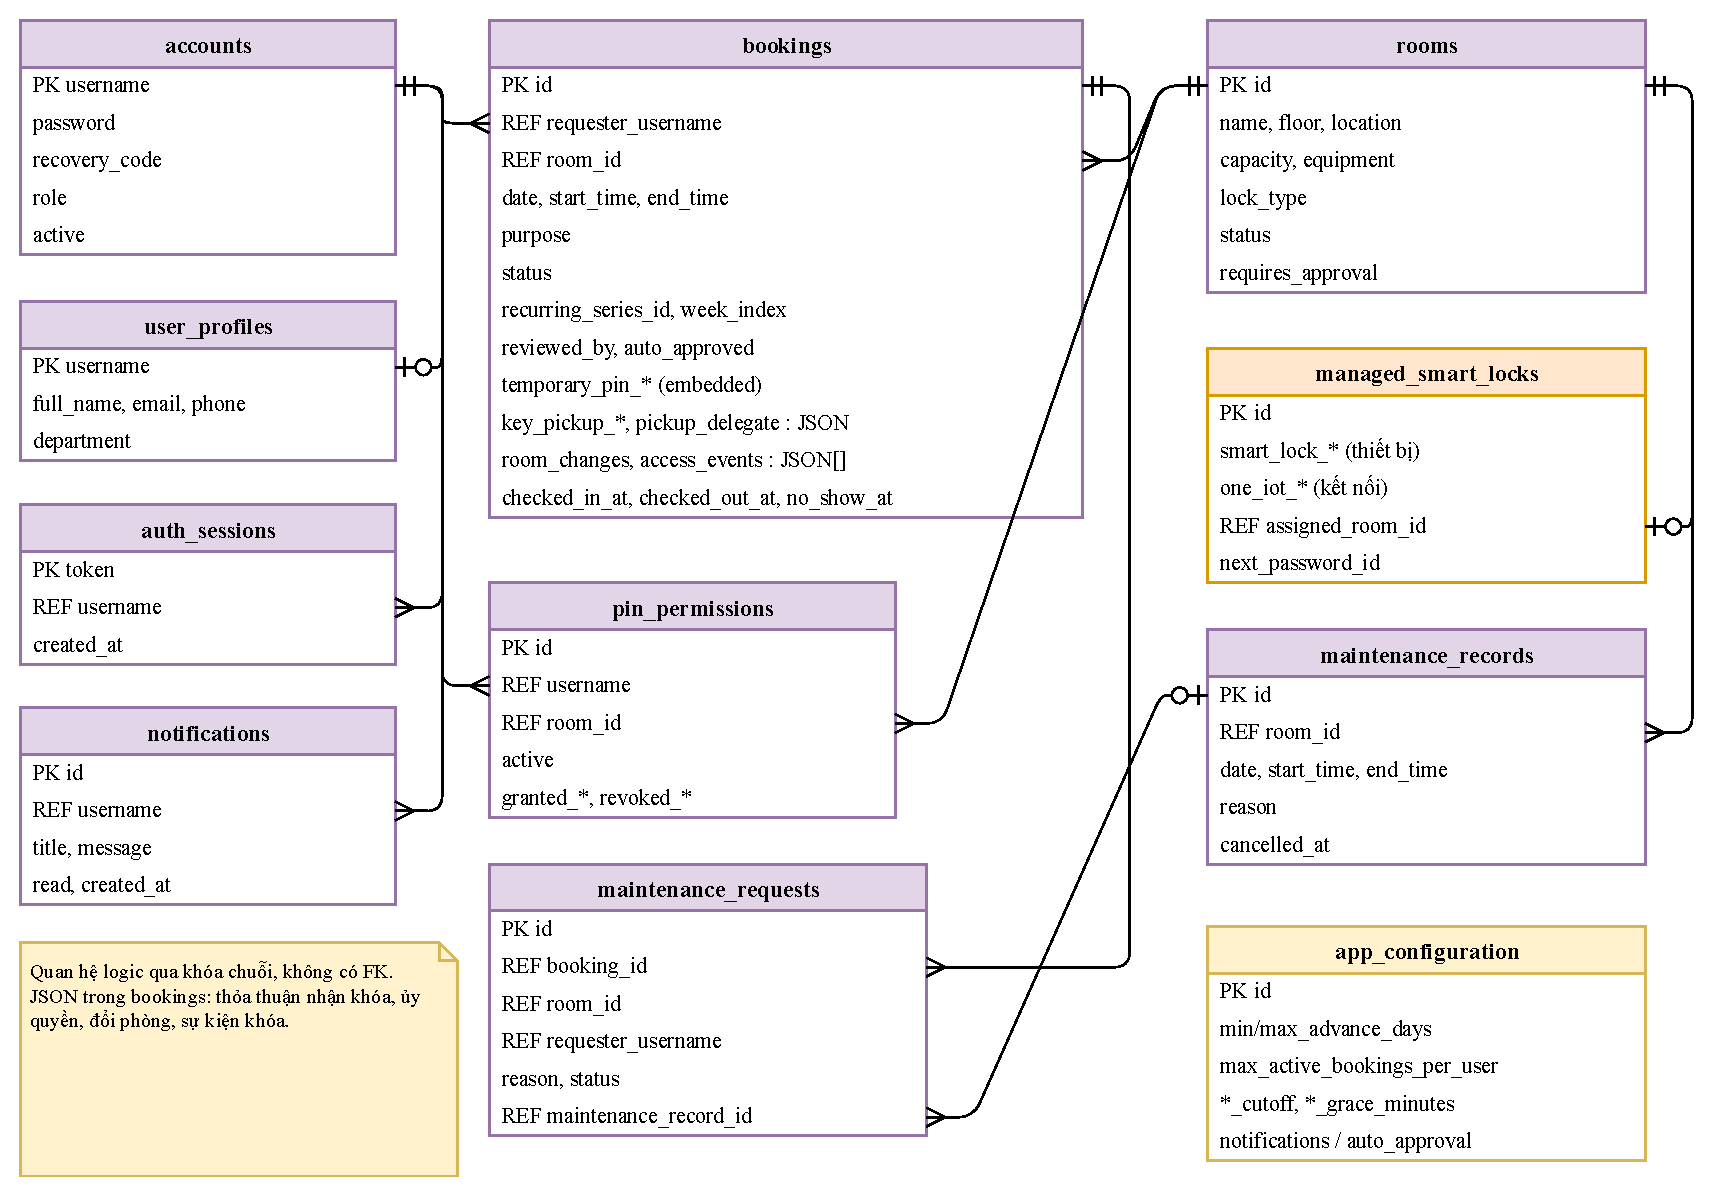
\includegraphics[width=.98\linewidth,height=.85\textheight,keepaspectratio]{Hinhve/design/17_er_diagram.pdf}
\caption{Mô hình thực thể và quan hệ logic của RoomHub}\label{fig:erd}
\end{figure}
\clearpage
\end{landscape}

\section{Quy trình tái lập kỹ thuật}\label{sec:technical-reproduction}
\subsection{Đóng gói Release trên macOS/Linux}
Các lệnh sau thực hiện tại \code{code/booking_classroom/}, sau khi cấu hình JDK/SDK, chọn nguồn dữ liệu và chạy \cmd{npm ci}. Bước bundle đưa JavaScript và tài nguyên vào APK trước khi Gradle đóng gói:
\begin{Verbatim}[fontsize=\small,frame=single,breaklines=true]
mkdir -p android/app/src/main/assets
node node_modules/react-native/cli.js bundle \
  --platform android --dev false --entry-file index.js \
  --bundle-output android/app/src/main/assets/index.android.bundle \
  --assets-dest android/app/src/main/res
cd android
sh ./gradlew assembleRelease
cd ..
\end{Verbatim}

Cài APK và mở ứng dụng theo mục 4.7. Trên Windows, script \cmd{npm run build:android:release} thực hiện các bước bundle và Gradle tương ứng.

\subsection{Tái lập kiểm thử}\label{sec:test-reproduction}
Các bộ ứng dụng, quality, quyền thông báo và kiểm tra tĩnh chạy từ thư mục ứng dụng; dữ liệu kết quả được lưu riêng cho từng bộ:
\begin{Verbatim}[fontsize=\small,frame=single,breaklines=true]
npm test -- --runInBand
npx jest --config quality-tests/jest.config.js --runInBand
npx jest --config ../../docs/reports/final/LTUD/minh_chung/kiem_thu/jest.permission.config.cjs --runInBand
npx tsc --noEmit
npm run lint
\end{Verbatim}

Kiểm thử backend dùng \cmd{mvn test} tại \code{code/booking-server/}. Môi trường, dữ liệu và kết quả thực nghiệm Android được lưu trong hồ sơ kiểm thử \cite{currenttests}; lệnh ADB và vị trí ảnh/XML đi kèm hồ sơ.

\FloatBarrier
\chapter{ĐỐI CHIẾU ĐÓNG GÓP THÀNH VIÊN}\label{app:contributions}
{\small\setstretch{1.0}\section{Đối chiếu từng thành viên}
Bảng này tổng hợp đầu việc, sản phẩm bàn giao và vị trí mã nguồn của từng thành viên. Cột đóng góp dùng tỷ lệ ở Bảng~\ref{tab:members}; số liệu mã nguồn và kiểm thử được trình bày ở Chương~\ref{chap:team}. Đường dẫn app tính từ \code{code/booking_classroom/}; đường dẫn Java tính từ \code{code/booking-server/src/main/java/com/bookingclassroom/server/}.
{\tabletext\renewcommand{\arraystretch}{1.04}\begin{longtable}{>{\raggedright\arraybackslash}p{\dimexpr0.18\textwidth-2\tabcolsep\relax}>{\raggedright\arraybackslash}p{\dimexpr0.3\textwidth-2\tabcolsep\relax}>{\raggedright\arraybackslash}p{\dimexpr0.35\textwidth-2\tabcolsep\relax}>{\raggedright\arraybackslash}p{\dimexpr0.17\textwidth-2\tabcolsep\relax}}
\caption{Đầu việc, sản phẩm và minh chứng thành viên}\label{tab:individual}\\
\toprule \textbf{Thành viên} & \textbf{Đầu việc và kết quả} & \textbf{Vị trí mã nguồn} & \textbf{Đóng góp}\\\midrule
\endfirsthead
\multicolumn{4}{l}{\small Đầu việc, sản phẩm và minh chứng thành viên (tiếp)}\\
\toprule \textbf{Thành viên} & \textbf{Đầu việc và kết quả} & \textbf{Vị trí mã nguồn} & \textbf{Đóng góp}\\\midrule
\endhead
\bottomrule\endlastfoot
Đỗ Thùy Linh & Phòng/lọc, API và chiếm chỗ; tổ chức controller theo chức năng, tiện ích giao giờ. & \code{src/modules/room_management/}; \code{src/core/time/intervals.ts}; backend: \code{api/}. & 26\%.\\\addlinespace[1.5pt]
Hoàng Văn Tùng & Khung app, điều hướng, xác thực, phòng/booking nền, PIN/native SmartLock; tích hợp và sửa hồi quy. & \code{App.tsx}; \code{src/app/}; \code{src/modules/auth/}; \code{src/modules/access_control/}; \code{src/modules/smart_lock/}. & 28\%.\\\addlinespace[1.5pt]
Nguyễn Việt Dũng & Bộ kiểm thử chất lượng và báo cáo test; tự duyệt phòng thường ở app/server. & \code{quality-tests/}; \code{src/modules/auto_approval/}; backend \code{AutoApprovalPolicy.java}. & 26\%.\\\addlinespace[1.5pt]
Nguyễn Đình Phúc & Lịch lặp, vắng mặt, màn duyệt/thông báo, sơ đồ và báo cáo. & \code{src/modules/booking/}; \code{src/modules/notifications/}; \code{design/}; báo cáo LTUD. & 20\%.\\\addlinespace[1.5pt]
\end{longtable}}

Các vị trí mã nguồn và tệp kiểm thử hỗ trợ kiểm tra sản phẩm bàn giao của từng thành viên. Tỷ lệ đóng góp bao gồm cả công việc thiết kế, tích hợp, thử nghiệm, tài liệu và phối hợp.

\section{Tái lập thống kê}
Dữ liệu thống kê được lưu trong \code{minh_chung/thong_ke_git.json}; script \code{minh_chung/thong_ke_git.py} hỗ trợ quy thuộc dòng theo tác giả từ lịch sử Git. Hướng dẫn chạy và thông tin kỹ thuật được lưu cùng script để tái lập khi cần.

\section[Công cụ hỗ trợ]{Công cụ hỗ trợ và tài nguyên bên ngoài}
React Native/React, TypeScript, Async Storage, Spring/JPA/H2, Jest và react-test-renderer được khai báo trong package/lockfile và đối chiếu ở Chương~\ref{chap:design}. Sơ đồ Draw.io, quy trình nghiệp vụ, mẫu ET4710 \cite{template4710}, ảnh ứng dụng của nhóm và dữ liệu phòng demo được dẫn tại Phụ lục~\ref{app:evidence}; ảnh minh họa quá trình sử dụng các chức năng của ứng dụng.
}
\end{document}
